% !Mode:: "TeX:UTF-8"
%!TEX program  = xelatex
%“华为杯”第十八届中国研究生数学建模竞赛论文格式规范:
%论文题目和摘要写在论文摘要上,摘要页的下一页开始论文正文;
%论文从摘要页开始编写页码,页码必须位于每页页脚中部,用阿拉伯数字从“1 ”开始连续编号;
%论文题目用三号黑体字、一级标题用四号黑体字,并居中;
%论文中其他汉字一律采用小四号宋体字,行距用单倍行距。计算机结果和源程序需在规定时间内上传竞赛系统以备检查。
%请大家注意:摘要应该是一份简明扼要的详细摘要(包括关键词),请认真书写(注意篇幅一般不超过两页,且无需译成英文)。全国评阅时对摘要和论文都会审阅。
%论文不能有页眉,论文中不能有任何可能显示答题人身份的标志。
\documentclass[a4paper,10pt]{my_paper}
\usepackage{ctex}
\usepackage[top=30.0mm,bottom=25.0mm,left=22.5mm,right=22.5mm,headsep=8mm]{geometry}%设置页边距
\usepackage{array} %主要是增加列样式选项
\usepackage[dvipsnames]{xcolor}%颜色宏包
\usepackage{graphicx}%图片宏包
\usepackage{amsmath}%公式宏包
\usepackage{float} %限制浮动体的位置
\usepackage{pdfpages}
\usepackage{listings}
\usepackage{titletoc}
\usepackage{booktabs}%表格宏包
\usepackage{rotating}%旋转宏包
\usepackage{shadowtext}%大赛标题加阴影
\usepackage{multirow}%表格内多行合并
\usepackage{booktabs}
\usepackage{threeparttable}%表格添加注释 
\usepackage{subfigure}%子图宏包
\renewcommand{\baselinestretch}{1.0} %设置单倍行距
\graphicspath{ {./figures/} } % 插图放在这个文件夹里面
\numberwithin{equation}{section}
\usepackage{newtxtext, newtxmath}  %使用Times New Roman 字体的方法

\lstset{
    language = Python,
    backgroundcolor = \color{yellow!10},    % 背景色:淡黄
    basicstyle = \small\ttfamily,           % 基本样式 + 小号字体
    rulesepcolor= \color{gray},             % 代码块边框颜色
    breaklines = true,                  % 代码过长则换行
    %numbers = left,                     % 行号在左侧显示
    %numberstyle = \small,               % 行号字体
    keywordstyle = \color{blue},            % 关键字颜色
    commentstyle =\color{green!100},        % 注释颜色
    stringstyle = \color{red!100},          % 字符串颜色
    frame =  tb,                  % 用(带影子效果)方框框住代码块
    showspaces = false,                 % 不显示空格
    columns = fixed,                    % 字间距固定
}

%--------------------正文----------------------
\begin{document}


\numberwithin{equation}{section}
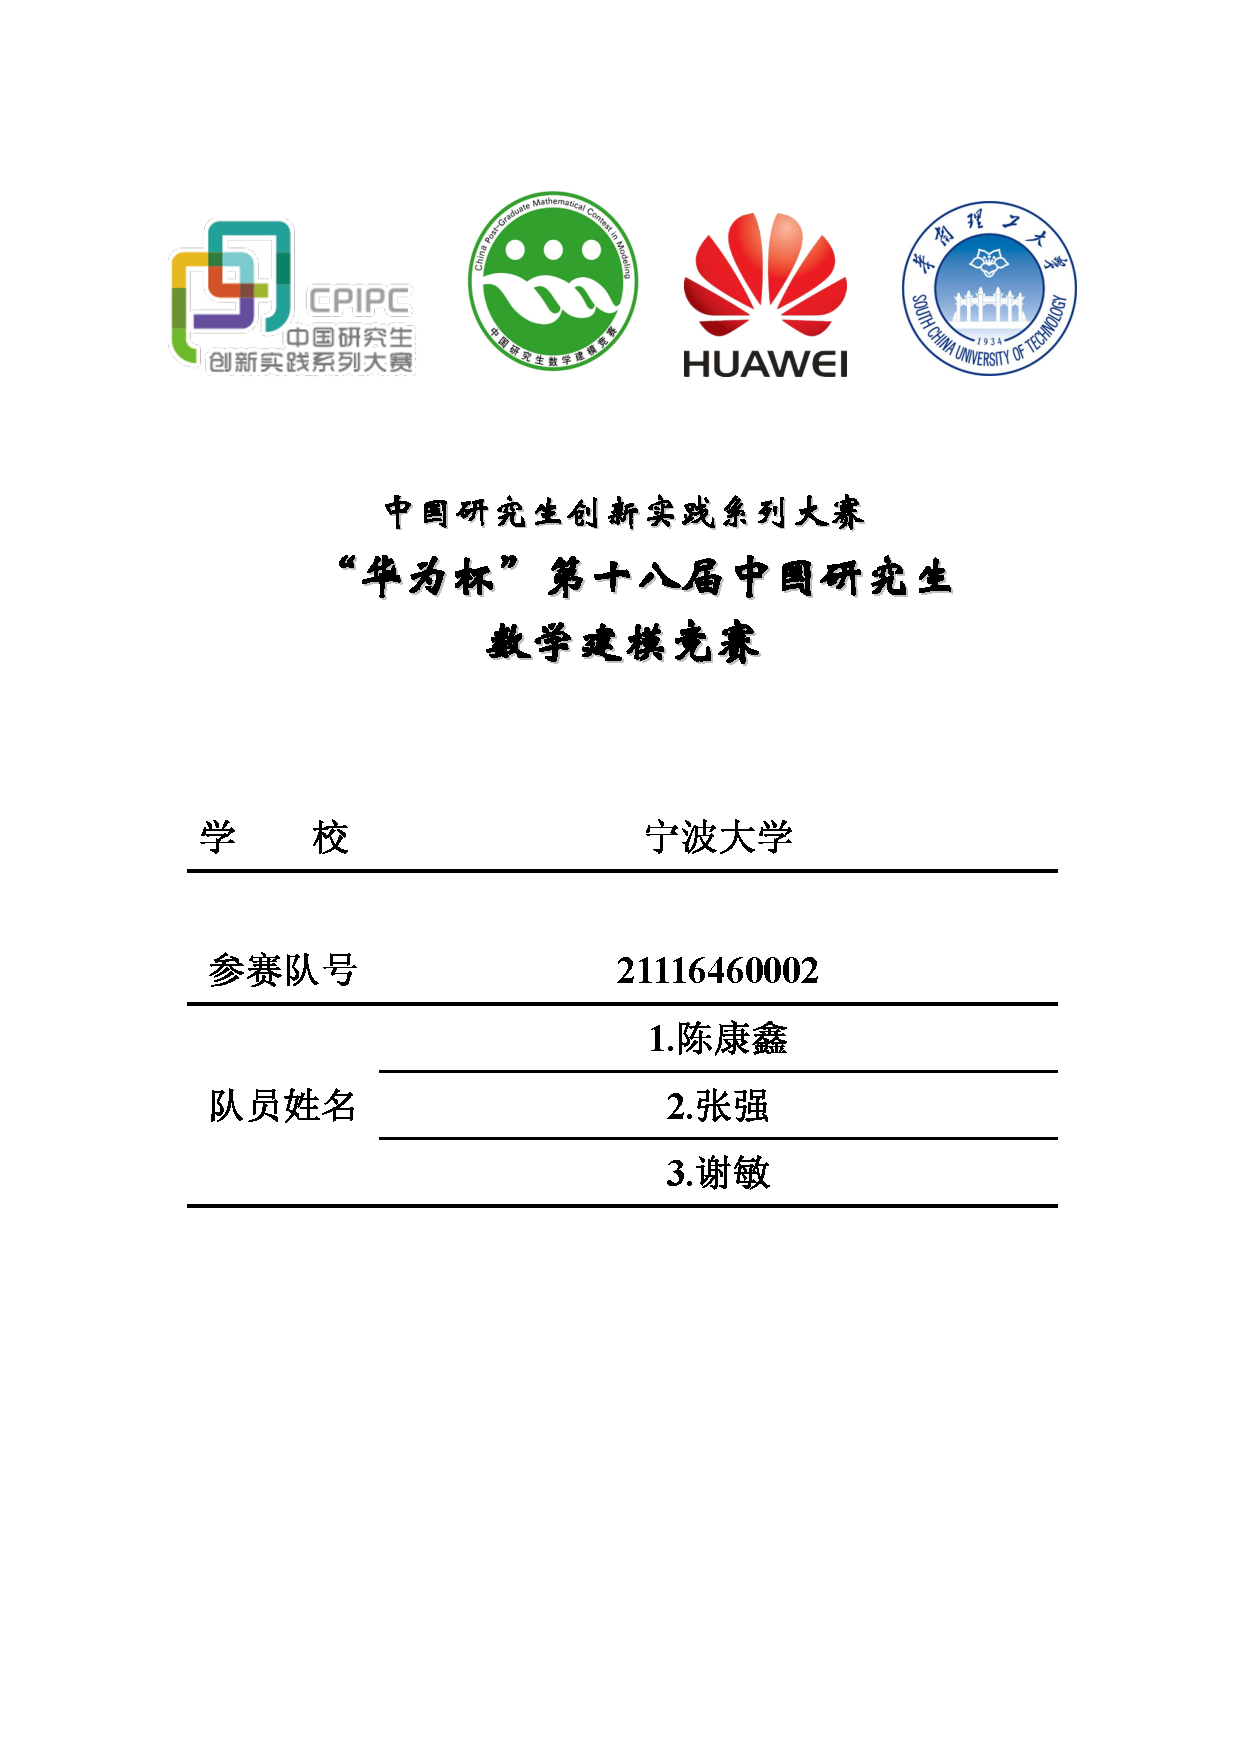
\includepdf[width=21cm]{titlepage}

%--------------------题目&摘要页----------------------
\newpage
\pagenumbering{arabic} %设置阿拉伯数字页码
\setcounter{page}{1} %正文为第一页

\begin{center}
    \zihao{-2}  \bfseries \xinwei \shadowtext{中国研究生创新实践系列大赛}

    \zihao{2} \shadowtext{\textbf{ \xinwei “华为杯”第十八届中国研究生}}

    \zihao{2} \shadowtext{\textbf{\xinwei 数学建模竞赛}}
    \end{center}

\vspace{1em}
\begin{tabular}{l p{0.8\textwidth}<{\centering}}
    \centering
    \zihao{4} 题\quad 目\quad & \zihao{3} \heiti 基于通信仿真的载波恢复算法设计与 ASIC 实现  \\ \cline{2-2}
\end{tabular}

\begin{center} \zihao{-2} \lishu 摘 \qquad 要:
\end{center}

本文研究了空气质量的二次预报问题,主要创新点在于:(1)(2)
%空行即换行
针对任务一,使用了基于半参数的差值网络模型来完成数据缺失值的处理,并结合箱型图提出异常值。结合给定的AQI计算方法求出了2020年8月25日到8月28日每天实测的AQI和首要污染物。

针对任务二,充分考虑了时间滞后性问题,通过计算各气象条件峰值与污染物浓度峰值的时间差,降低了时间滞后性带来的AQI计算不准确性。在计算了AQI之后,通过AQI的等级,将污染物分成了3类,

针对任务三,首先根据问题描述的A、B、C之间的影响忽略不计而舍弃掉对地理位置有影响的近地风向这一解释变量,接着通过分析各数据的。

针对任务四,为了实现位宽自动优化并综合考虑性能和资源两种因素,考虑到资源与
芯片实现面积和功耗有关,首先建立资源使用量化评价函数。然后以 RSNR 代价作为性能
评定指标,以不同位宽向量下的 RSNR 代价与资源使用评价函数分别赋予权重因子,组成
综合评价目标函数。最后提出基于禁忌搜索算法的位宽自动优化方法,以得到性能和代价
综合评价目标函数的最优 Pareto 解集,即最优位宽设计方案。

最后本文对 CR 算法的相位噪声提取效果以及整个信号传输系统的抗噪声性能进行了
检验,检验结果为:该算法能较好地提取出信道中的相位噪声;该算法提高了整个系统的
抗噪声性能。
                                                                                    
\vspace{1em}
\noindent \textbf{关键词:}仿真框架;CR 算法;噪声耦合;去耦合;ASIC 算法设计;量化噪声



%--------------------目录----------------------
\newpage

\begin{center}
\tableofcontents
\end{center}

%--------------------正文----------------------
%--------------------问题重述----------------------
\newpage
\section{问题重述}
\subsection{问题背景}

大气污染系指由于人类活动或自然过程引起某些物质进入大气中,呈现足够的浓度,达到了足够的时间,并因此危害了人体的舒适、健康和福利或危害了生态环境\cite{ref1}。污染防治实践表明,建立空气质量预报模型,提前获知可能发生的大气污染过程并采取相应控制措施,是减少大气污染对人体健康和环境等造成的危害,提高环境空气质量的有效方法之一。

目前常用WRF-CMAQ模拟体系(以下简称WRF-CMAQ模型)对空气质量进行预报。WRF-CMAQ模型主要包括WRF和CMAQ两部分:WRF是一种中尺度数值天气预报系统,用于为CMAQ提供所需的气象场数据;CMAQ是一种三维欧拉大气化学与传输模拟系统,其根据来自WRF的气象信息及场域内的污染排放清单,基于物理和化学反应原理模拟污染物等的变化过程,继而得到具体时间点或时间段的预报结果。

但受制于模拟的气象场以及排放清单的不确定性,以及对包括臭氧在内的污染物生成机理的不完全明晰,WRF-CMAQ预报模型的结果并不理想。因此题目提出了二次建模概念:即指在WRF-CMAQ等一次预报模型模拟结果的基础上,结合更多的数据源进行再建模,以提高预报的准确性。

针对一次预测不准确的问题,本文二次建模的主要目的有:一是结合已有数据与一次预测结果对二次污染物的生成进行分析;二是提升预测精度。

\subsection{问题提出}
通过数学建模,解决了以下问题:

\textbf{任务一:}使用附件1中的数据,按照附录中的方法计算监测点A从2020年8月25日到8月28日每天实测的空气质量指数(Air QUality Index, AQI)和首要污染物,将结果按照附录“AQI计算结果表”的格式放在正文中。

\textbf{任务二:}在污染物排放情况不变的条件下,某一地区的气象条件有利于污染物扩散或沉降时,该地区的AQI会下降,反之会上升。使用附件1中的数据,根据对污染物浓度的影响程度,对气象条件进行合理分类,并阐述各类气象条件的特征。

\textbf{任务三:}使用附件1、2中的数据,建立一个同时适用于A、B、C三个监测点(监测点两两间直线距离>100km,忽略相互影响)的二次预报数学模型,用来预测未来三天6种常规污染物单日浓度值,要求二次预报模型预测结果中AQI预报值的最大相对误差应尽量小,且首要污染物预测准确度尽量高。并使用该模型预测监测点A、B、C在2021年7月13日至7月15日6种常规污染物的单日浓度值,计算相应的AQI和首要污染物,将结果依照附录“污染物浓度及AQI预测结果表”的格式放在论文中。

\textbf{任务四:}相邻区域的污染物浓度往往具有一定的相关性,区域协同预报可能会提升空气质量预报的准确度。如图 4,监测点A的临近区域内存在监测点A1、A2、A3,使用附件1、3中的数据,建立包含A、A1、A2、A3四个监测点的协同预报模型,要求二次模型预测结果中AQI预报值的最大相对误差应尽量小,且首要污染物预测准确度尽量高。使用该模型预测监测点A、A1、A2、A3在2021年7月13日至7月15日6种常规污染物的单日浓度值,计算相应的AQI和首要污染物,将结果依照附录“污染物浓度及AQI预测结果表”的格式放在论文中。并讨论:与问题3的模型相比,协同预报模型能否提升针对监测点A的污染物浓度预报准确度?说明原因。
%--------------------模型假设----------------------
\section{模型假设}
1. 假设近地面臭氧污染形成机制中的化学反应实现了完全转化;

2. 假设臭氧浓度数值在二次污染中,只受给定的气象数据以及其余五项污染物的浓度影响,汽车尾气、工业生产、全球变化等题目中未出现的影响因素不在本模型的考虑范围内;

3. 本文以 ${O_3-8h}$的滑动平均值为一次臭氧的空气质量影响,不进行${O_3-1h}$的空气质量评价;

4. 假设在二次污染期间,高层大气中的氧气不会经过系列转化形成新的臭氧;

5. 假设在二次污染期间,没有雷雨天气产生臭氧;

6. 假设空气质量只受地表臭氧浓度影响,高空如平流层的臭氧浓度不影响空气质量的判定;

7. {\color{red}假设四季变化对空气质量没有影响??}

8. 假设本文的二次污染物只有臭氧,没有有机颗粒物等其他污染物质;

9. 假设二次污染时,臭氧的形成只需考虑${NO_2}$的含量影响,不需要考虑${VOCs}$以及${NO_x}$的含量影响;

10. 假设本文模型不受地形特点影响;

%--------------------符号说明----------------------
\section{符号说明}

%使用三线表格最好~

%插入表格B站教程:https://www.bilibili.com/video/BV1p3411q7qG?spm_id_from=333.999.0.0、https://www.bilibili.com/video/BV1544y1b7dS?spm_id_from=333.999.0.0

\begin{table}[htb]
    \centering
    \begin{tabular}{p{2.0cm}<{\centering}p{9.0cm}<{\centering}p{2.0cm}<{\centering}}
 %指定单元格宽度, 并且水平居中。
    \hline
    符号 & 说明 & 单位 \\ %换行 
    \hline
    $\hat{S}$ & 接受信号 & V \\ %把你的符号写在这
    $S$ & 发送信号 & V \\ 
    $S_{16QAM}(t)$ &  经 16QAM 调制后的信号 &  V \\ 
    \hline
    \end{tabular}
\end{table}

%--------------------模型准备----------------------
%数学公式保姆级B站教程:https://www.bilibili.com/video/BV19f4y1n7ti?spm_id_from=333.999.0.0、https://www.bilibili.com/video/BV1F3411z7iD?spm_id_from=333.999.0.0
\section{模型准备}
(注意:这个部分根据自己的情况选择保留与否)



\begin{equation}
S_{16QAM}(t)=A_0 a_i\cos{\omega_0 t}+A_0 b_i\sin{\omega_0 t}=\sqrt{E_0}a_i \varphi_1(t)+\sqrt{E_0}b_i \varphi_2(t)
\end{equation}

\begin{align}
d_{16QAM}=\frac{\sqrt{2}}{L-1}=\frac{\sqrt{2}}{\sqrt{M}-1}=3\sqrt{2}
\intertext{式中:$L-QAM$ 信号比特位长;$M-QAM$ 电平数} \notag
\end{align}

%--------------------问题一的模型建立与求解----------------------

\section{问题一的模型建立与求解}
\subsection{问题一的描述分析}
问题一要求利用题目所提供的数据和公式,计算空气质量指数。题目提供的数据来自监测点长期空气质量预报基础数据,包括污染物浓度一次预报数据、气象一次预报数据、气象实测数据和污染物浓度实测数据。本文首先对给定数据进行了可视化分析,发现存在缺失值以及异常值,针对异常值采用了箱型图剔除法;针对缺失值,采用了基于半参数的插值网络,该网络充分考虑了时序性问题。在完成数值的预处理后利用给定的AQI计算方式完成问题一的求解。

\subsection{数据预处理}
在计算实测污染物的AQI之前,需要对数据进行统一的预处理,即\textbf{数据清洗}。其中,缺失值是本文主要处理的对象。从缺失数据的缺失影响因素来看,分为完全随机缺失(Missing Completely At Random, MCAR)、随机缺失(Missing At Random, MAR)、非随机缺失(Missing Not At Random, MNAR)角度考虑\textsuperscript{\cite{ref2}}。一般来说,如果数据中缺失观测值的比例相对于观测值总数很小,最简单的方式是删除带有缺失项的样本,即完全数据分析。当缺失项较多时,由于一部分的数据信息缺失,完全数据分析方法的偏差很大。如本课题中,附件2中监测点C逐小时污染物浓度与气象实测数据中湿度信息的缺失就有6147条,缺失比率占整个湿度信息的${31.6\%}$,直接删除包含缺失值的行可能会导致放弃有用的信息。从图\ref{fig_缺失图}题目给定信息的数据缺失量化图可以看出,信息数据的丢失比较多,不能简单的将缺失值进行丢弃。除开缺失值外,还有异常数据,图\ref{fig_异常值}为六个监测点A、B、C、A1、A2的六个污染物浓度的箱型图,其余信息的箱型图请见附件,针对异常值的处理,本文采用箱型图进行剔除。

% 图 1 
\begin{figure}[htb]
  \center{
  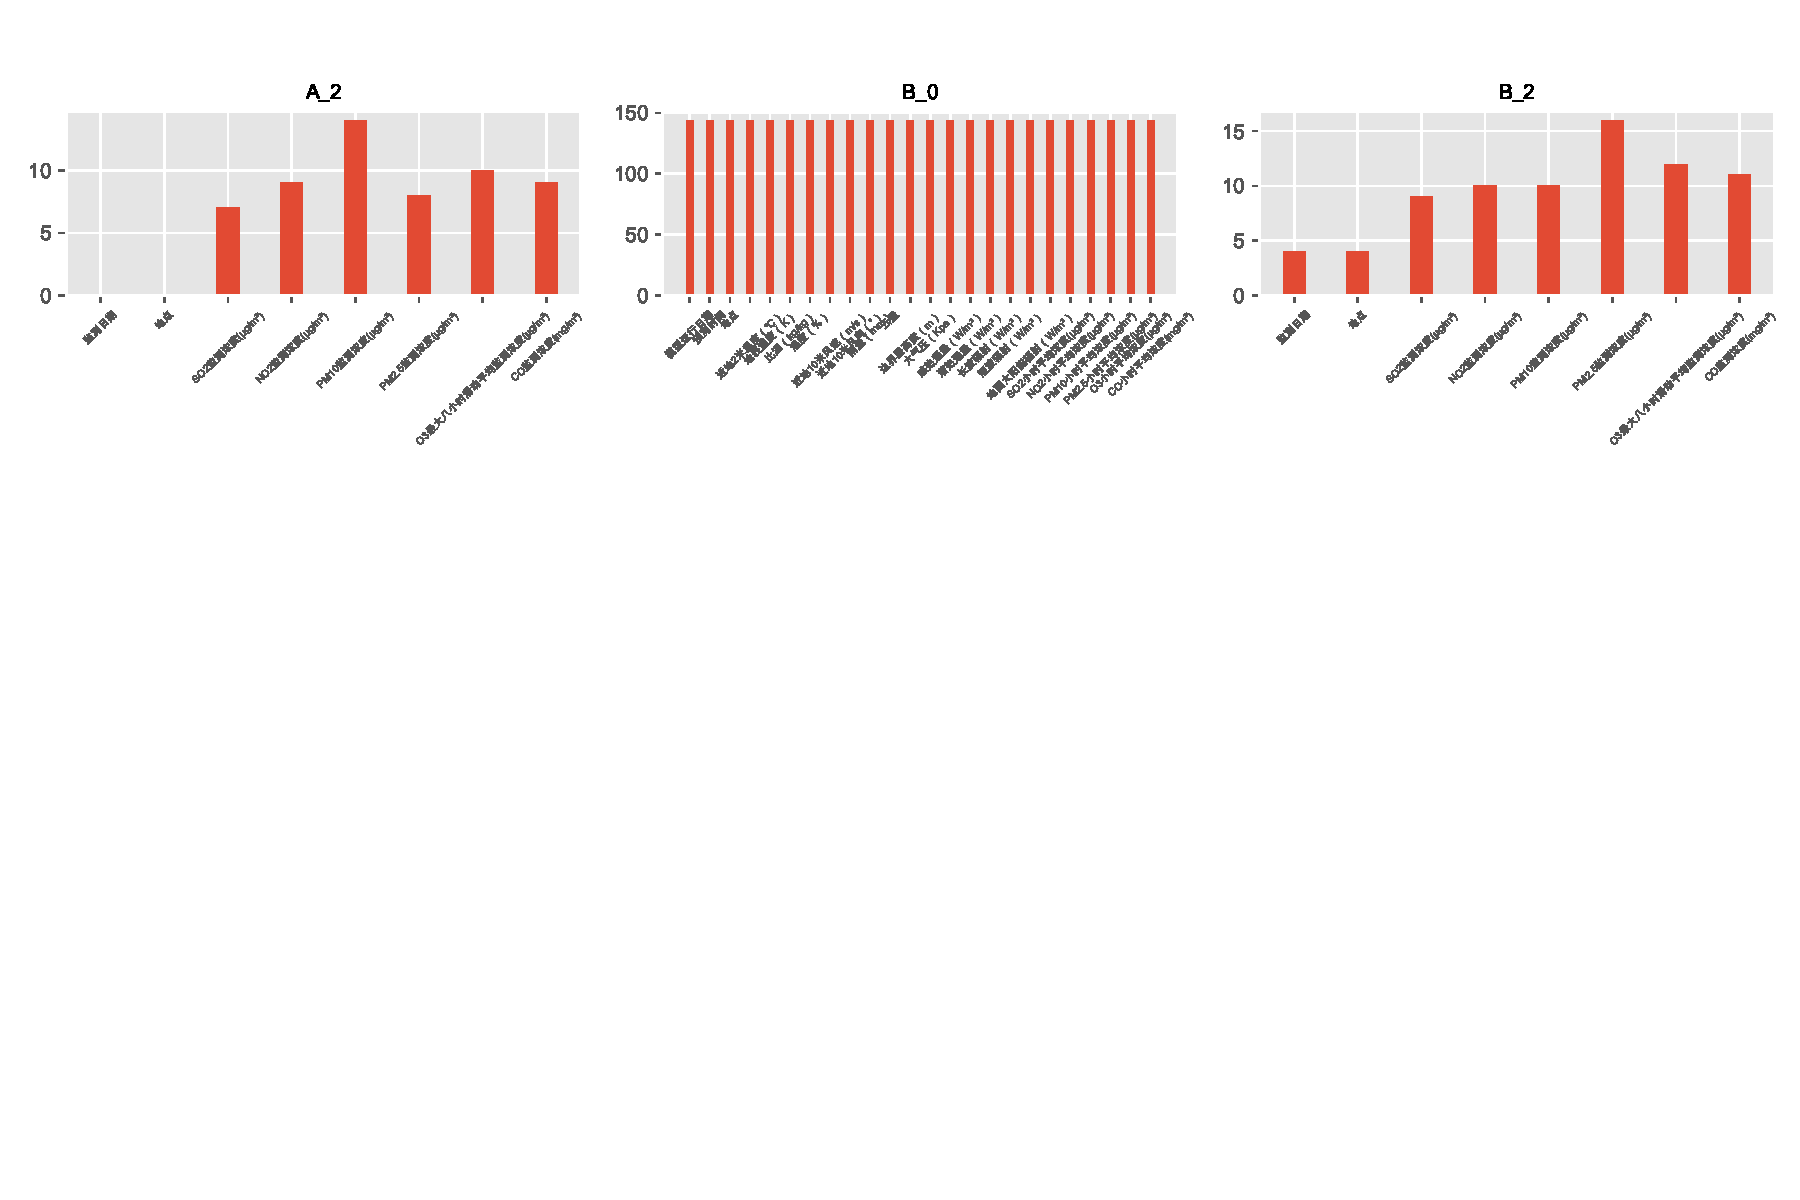
\includegraphics[width=1\textwidth]{Null_value0.pdf}\\
  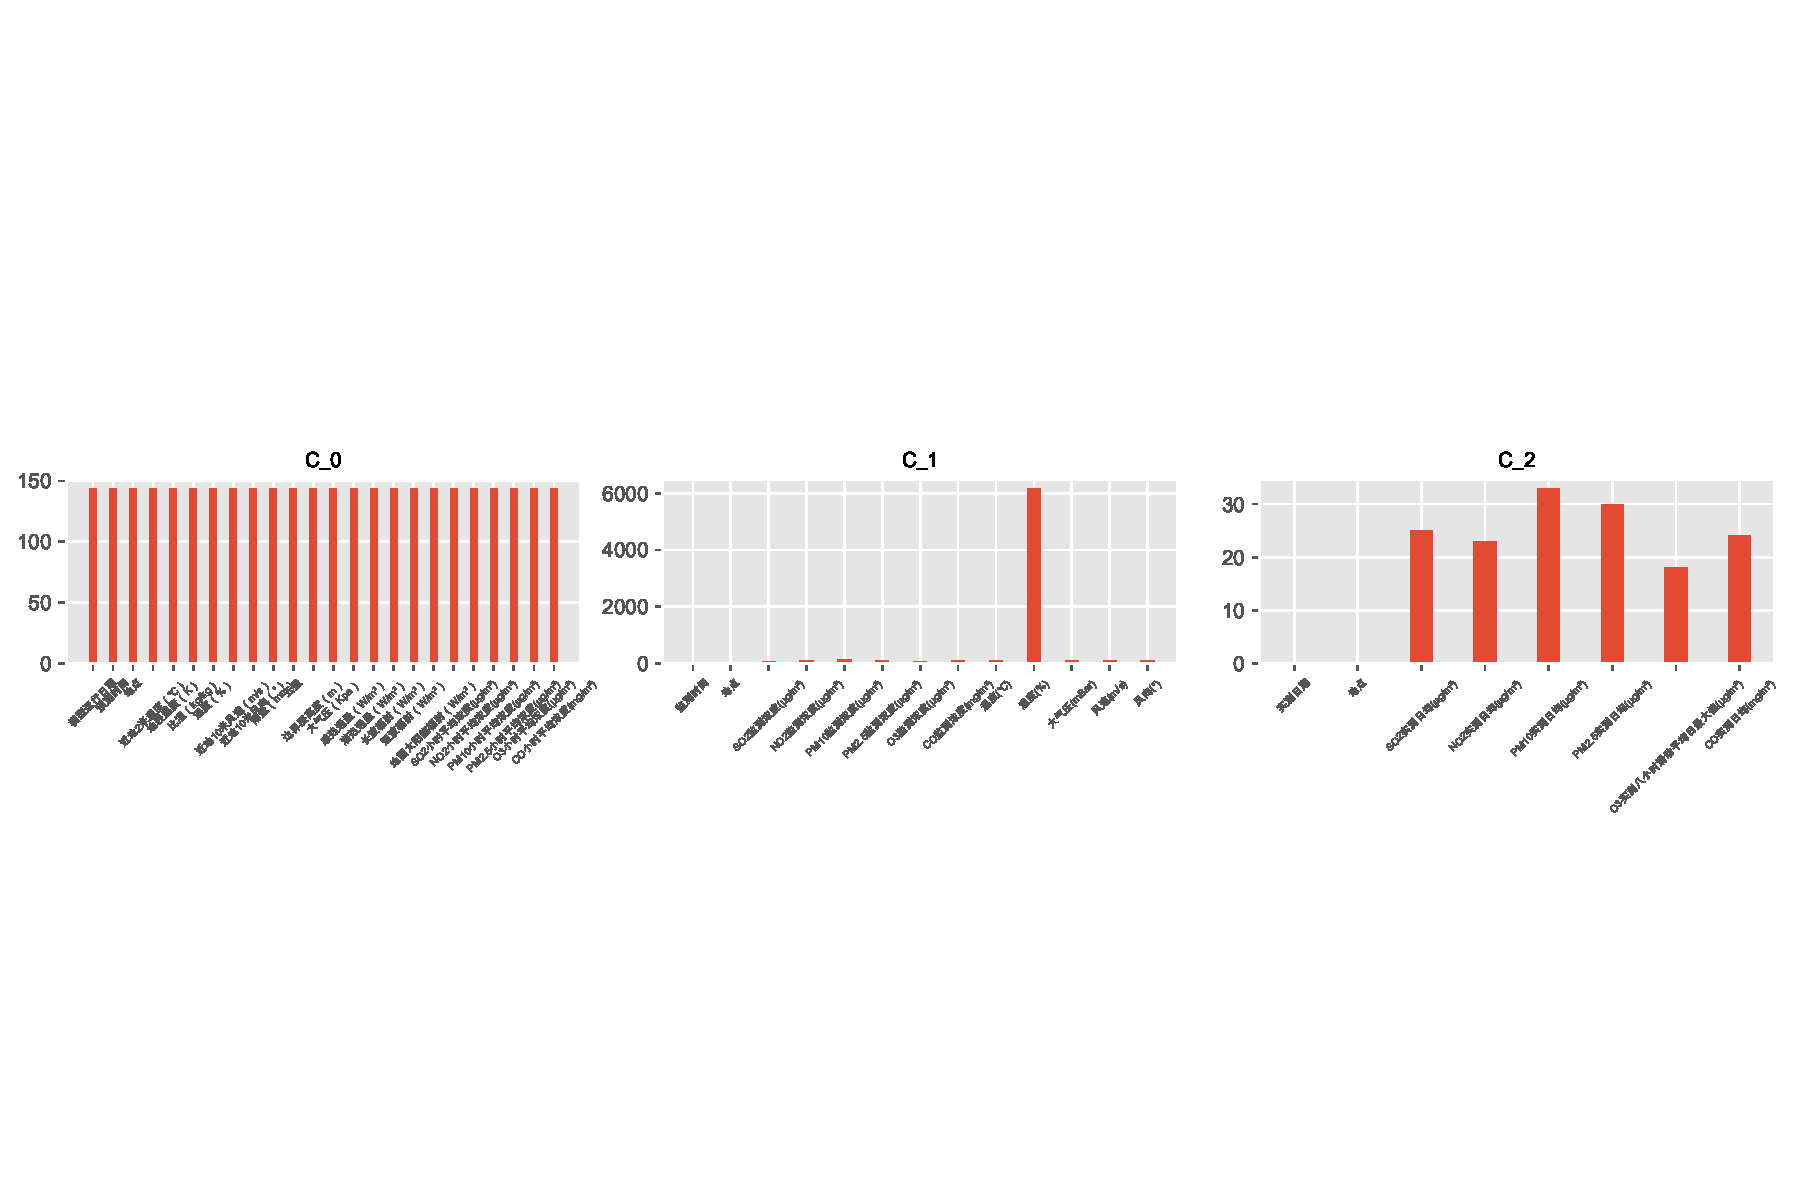
\includegraphics[width=1\textwidth]{Null_value1.pdf}\\
  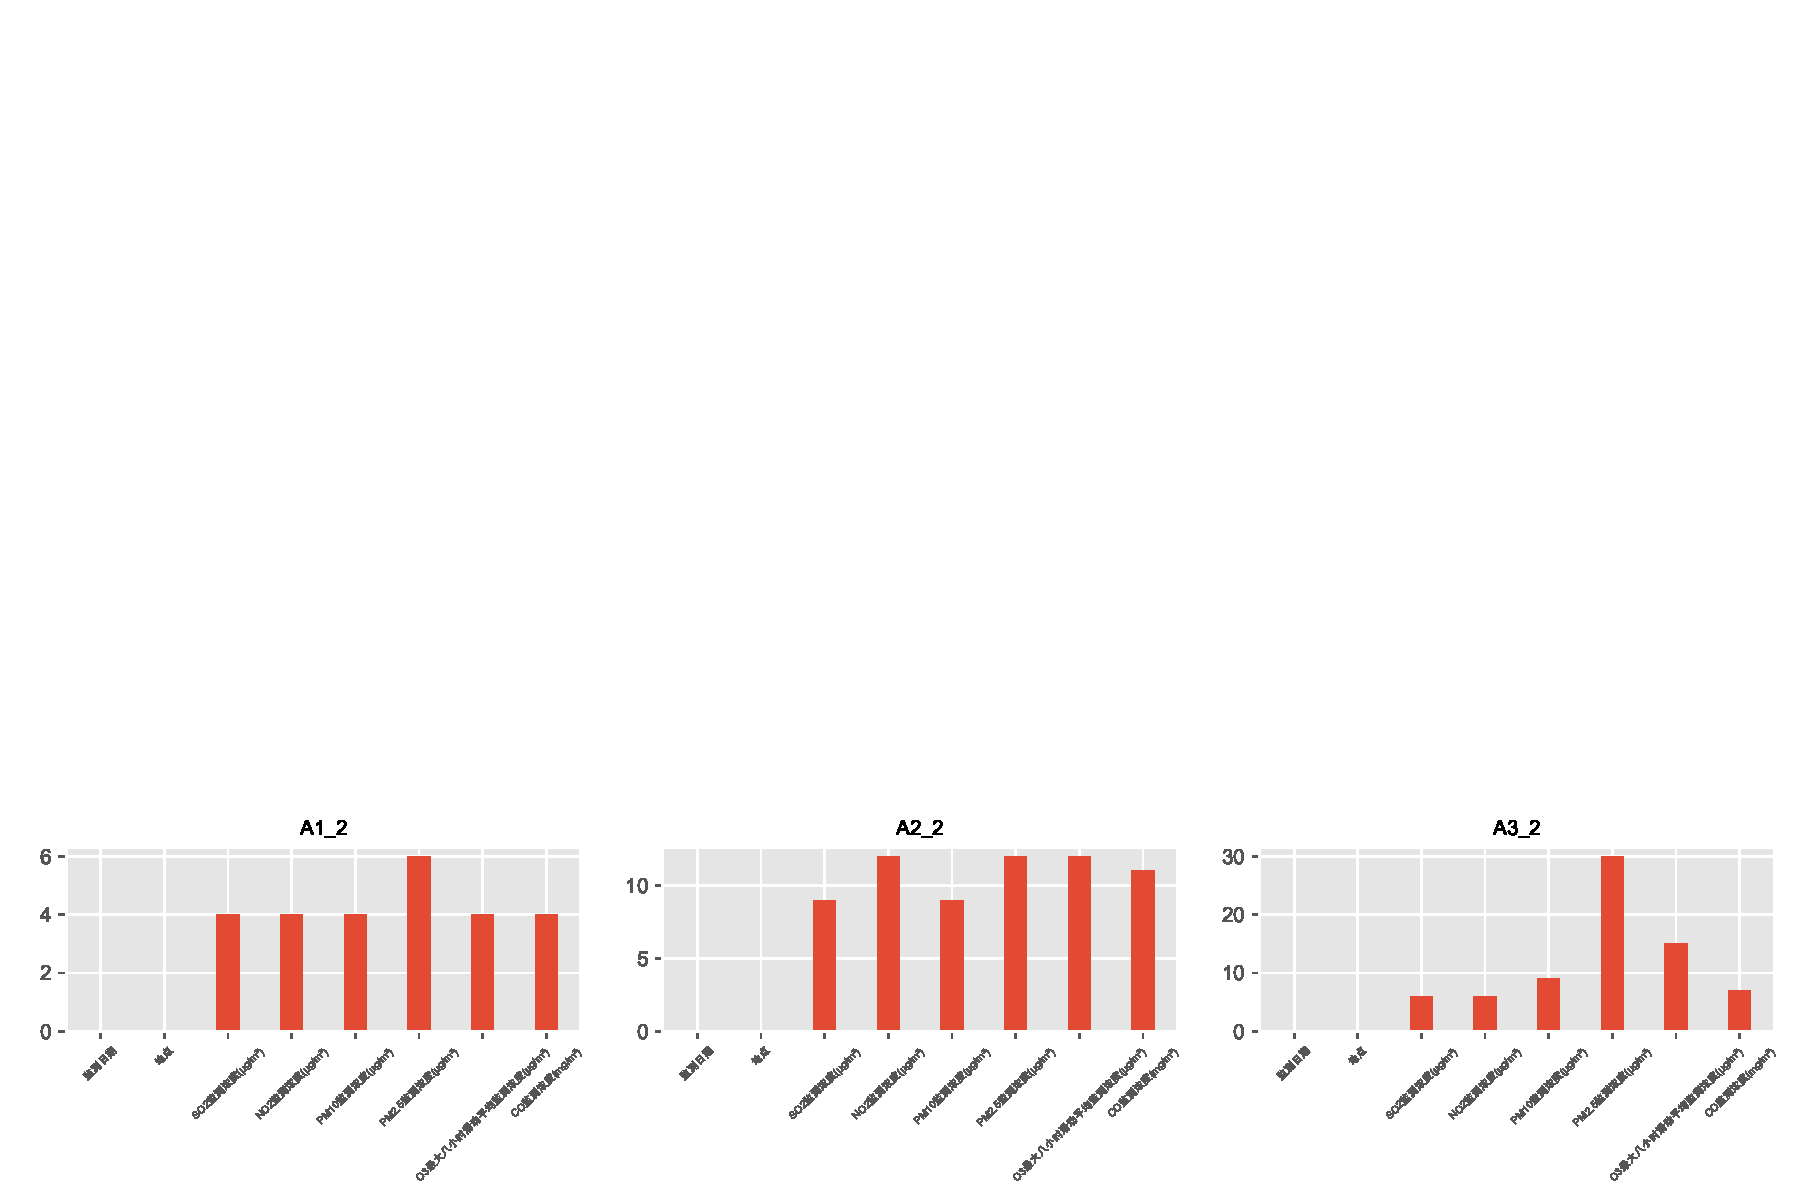
\includegraphics[width=1\textwidth]{Null_value2.pdf}
  }
  \caption{数据缺失量化图}\label{fig_缺失图}
\end{figure}

% 图 2 
\begin{figure}[htb]
  \center{
  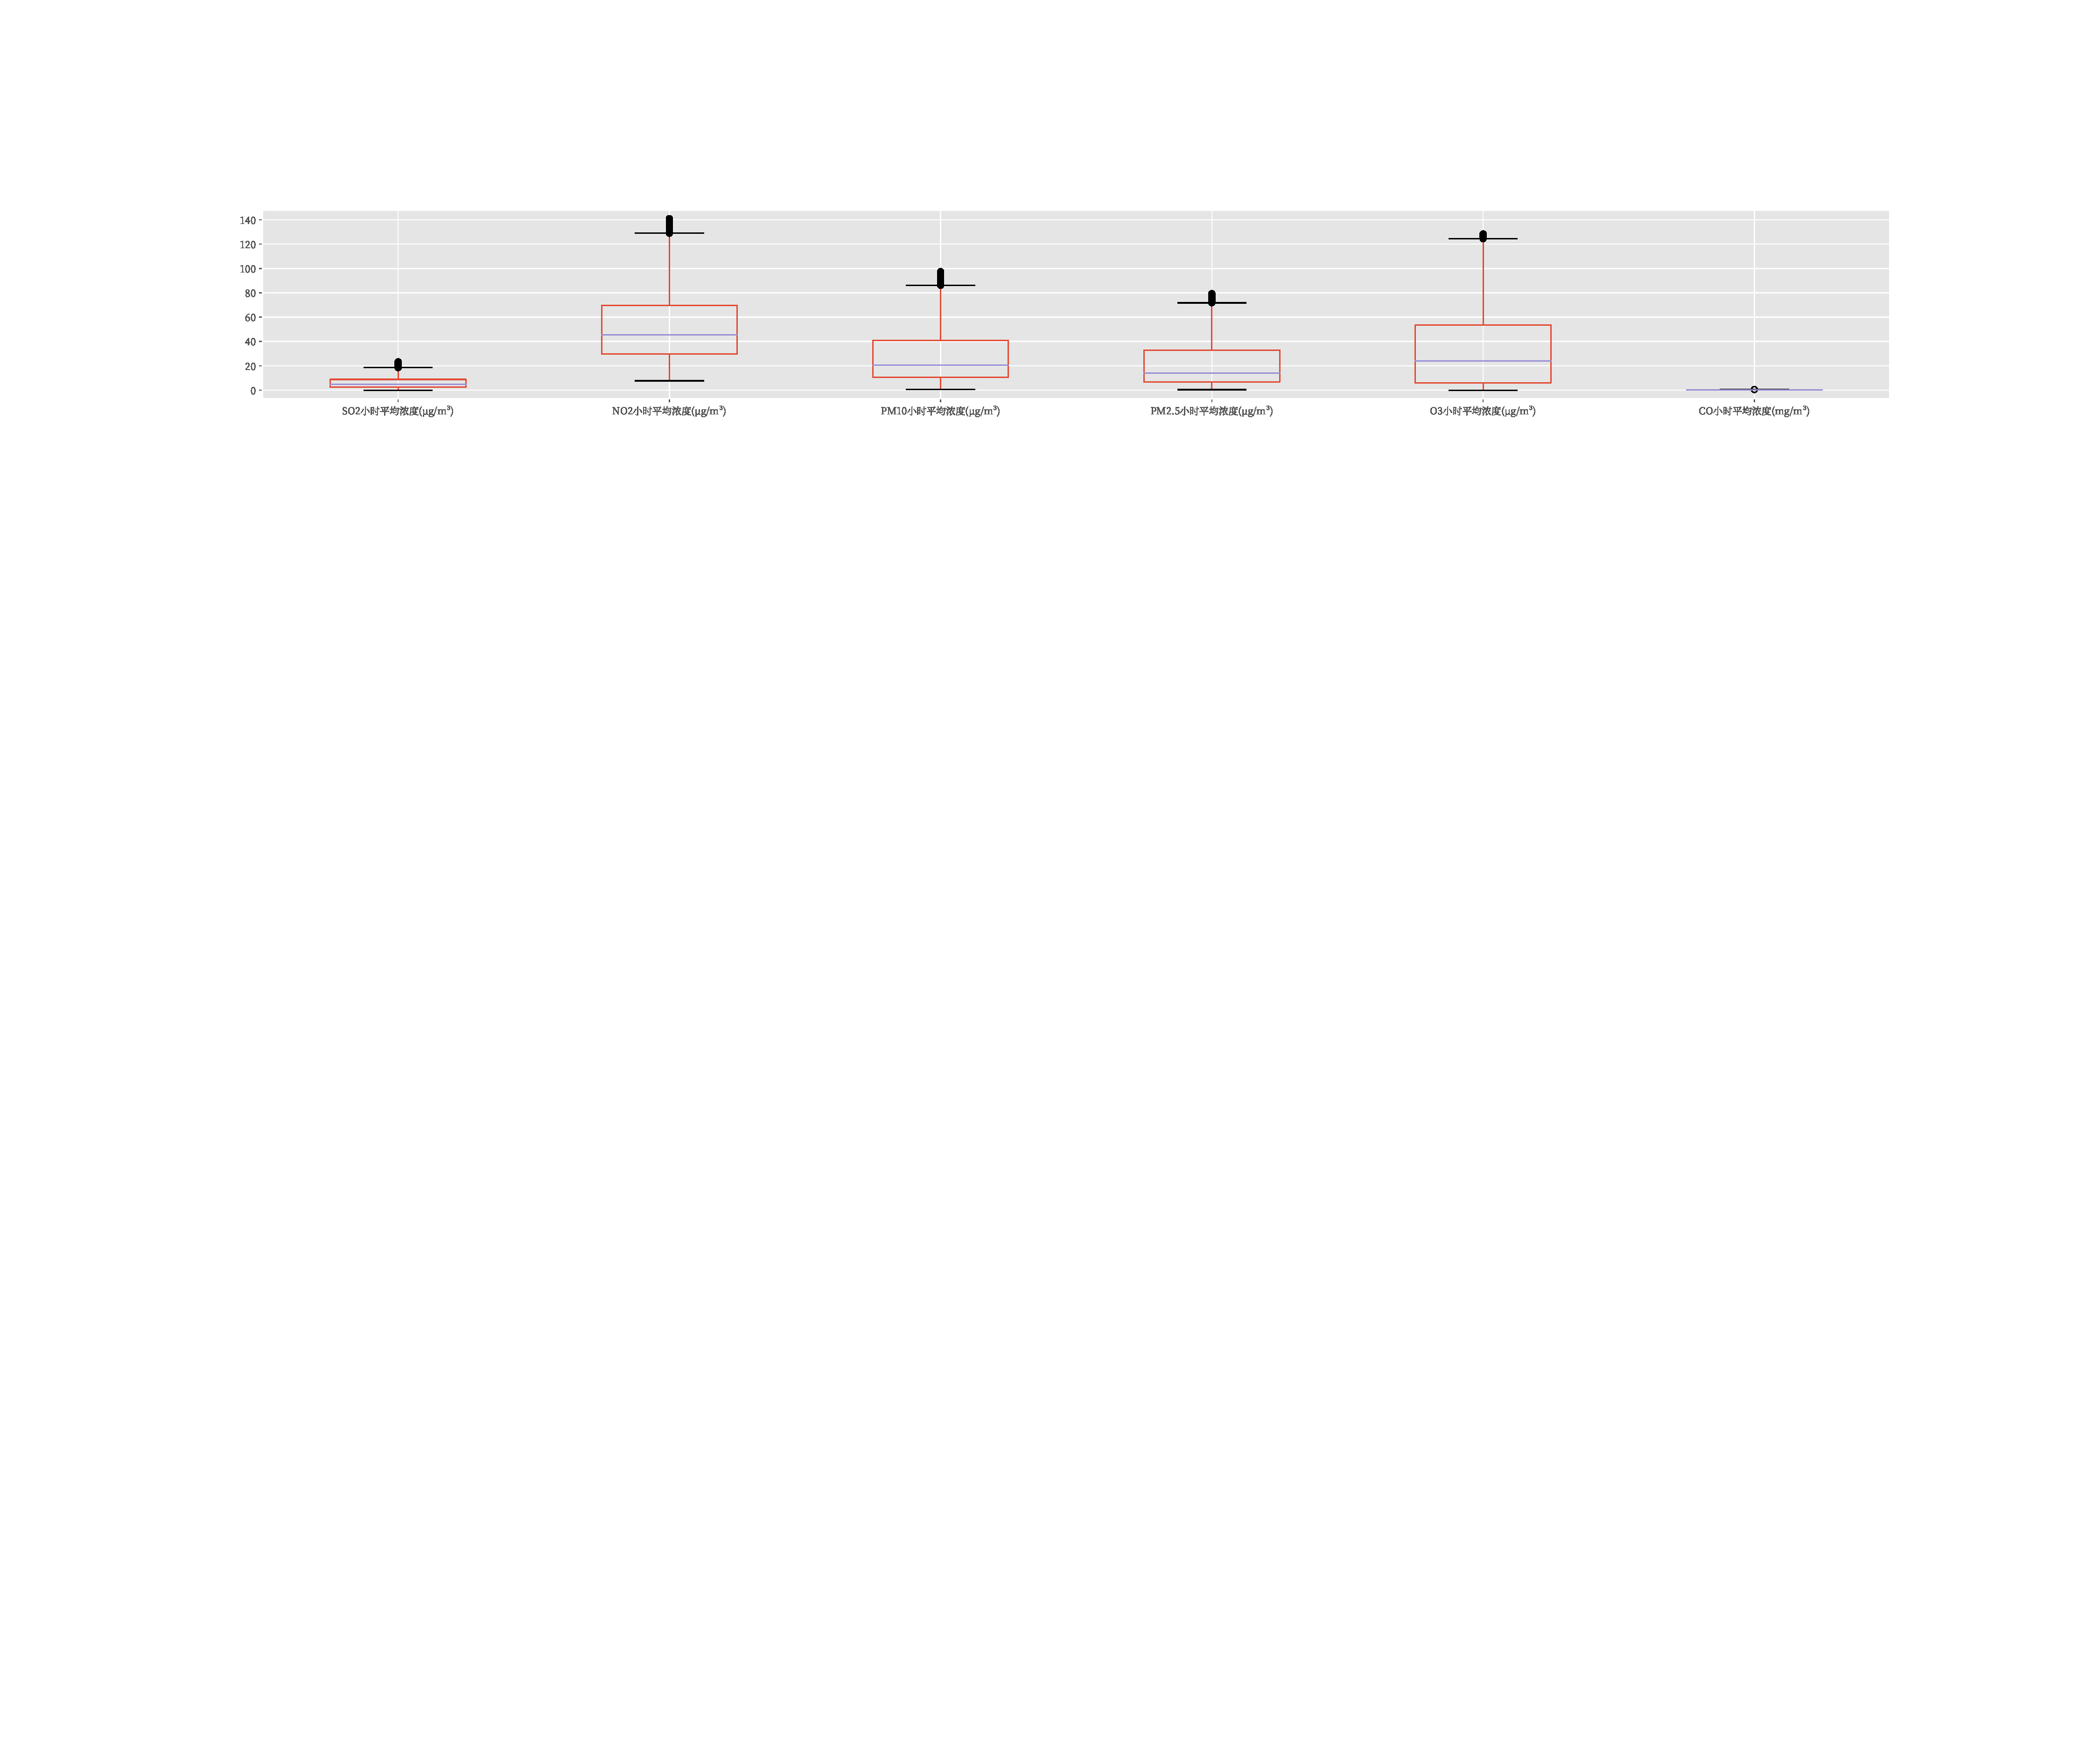
\includegraphics[width=1\textwidth]{box_plot_for_A.pdf}\\
  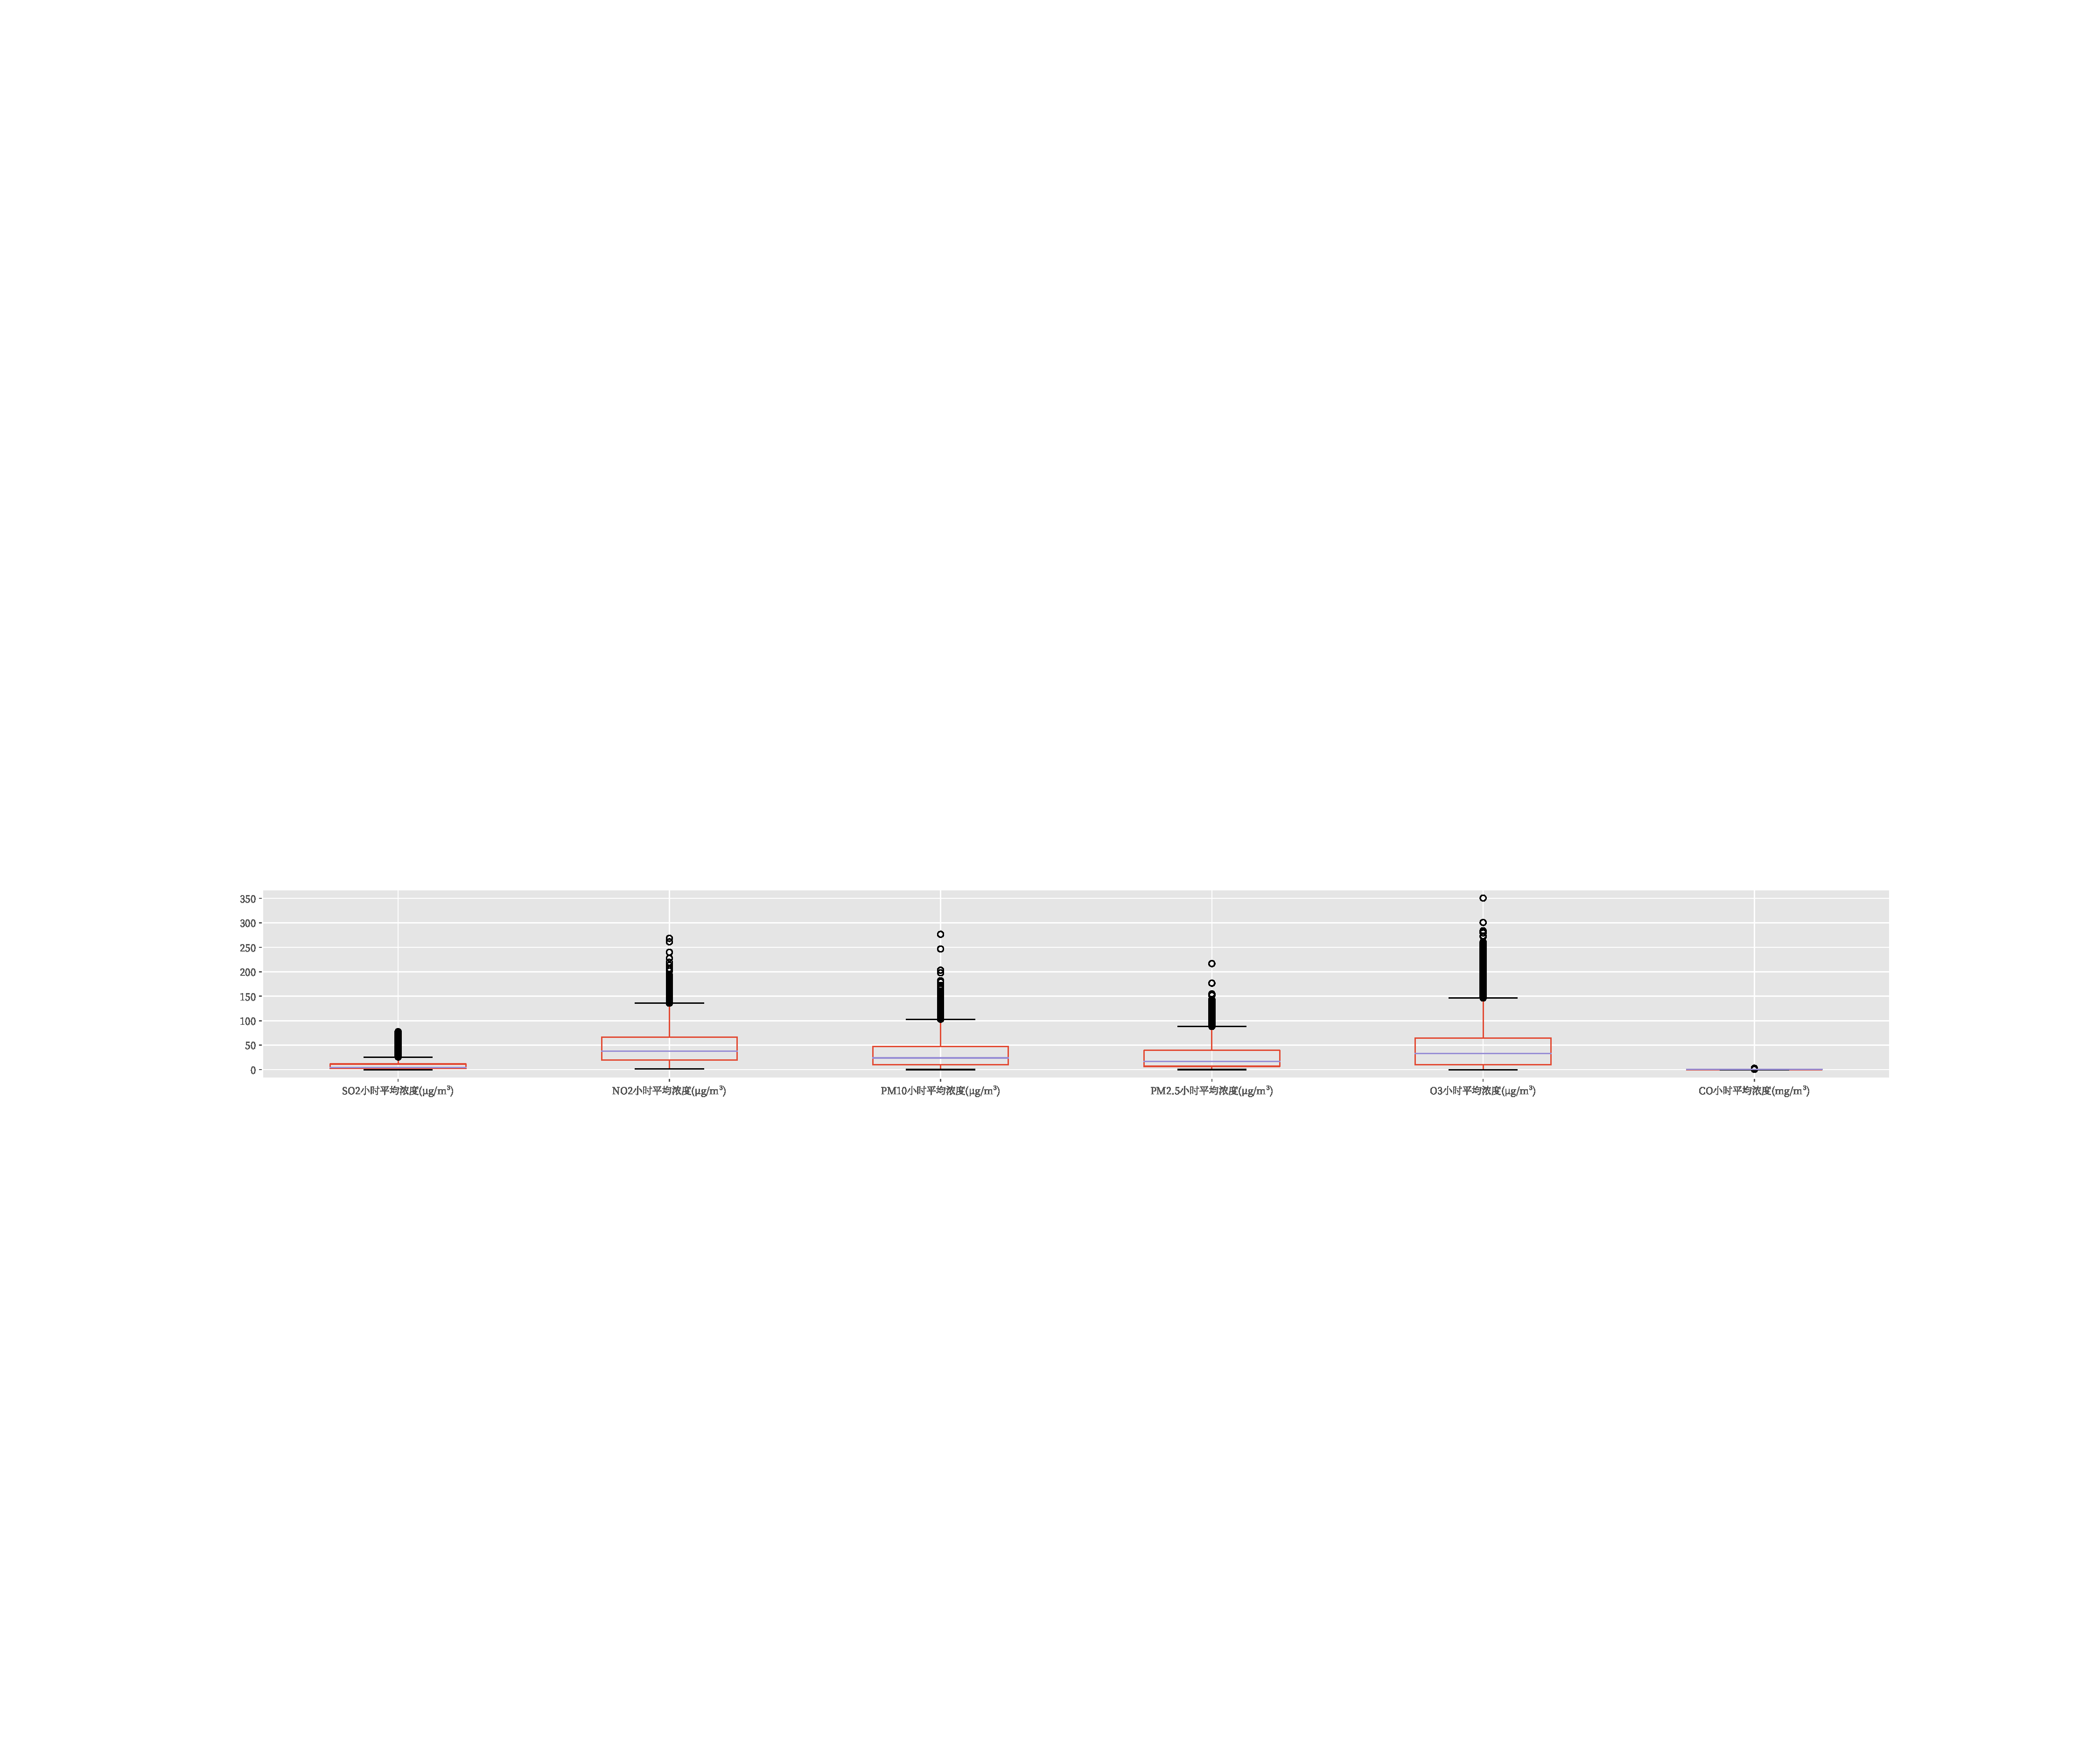
\includegraphics[width=1\textwidth]{box_plot_for_A1.pdf}\\
  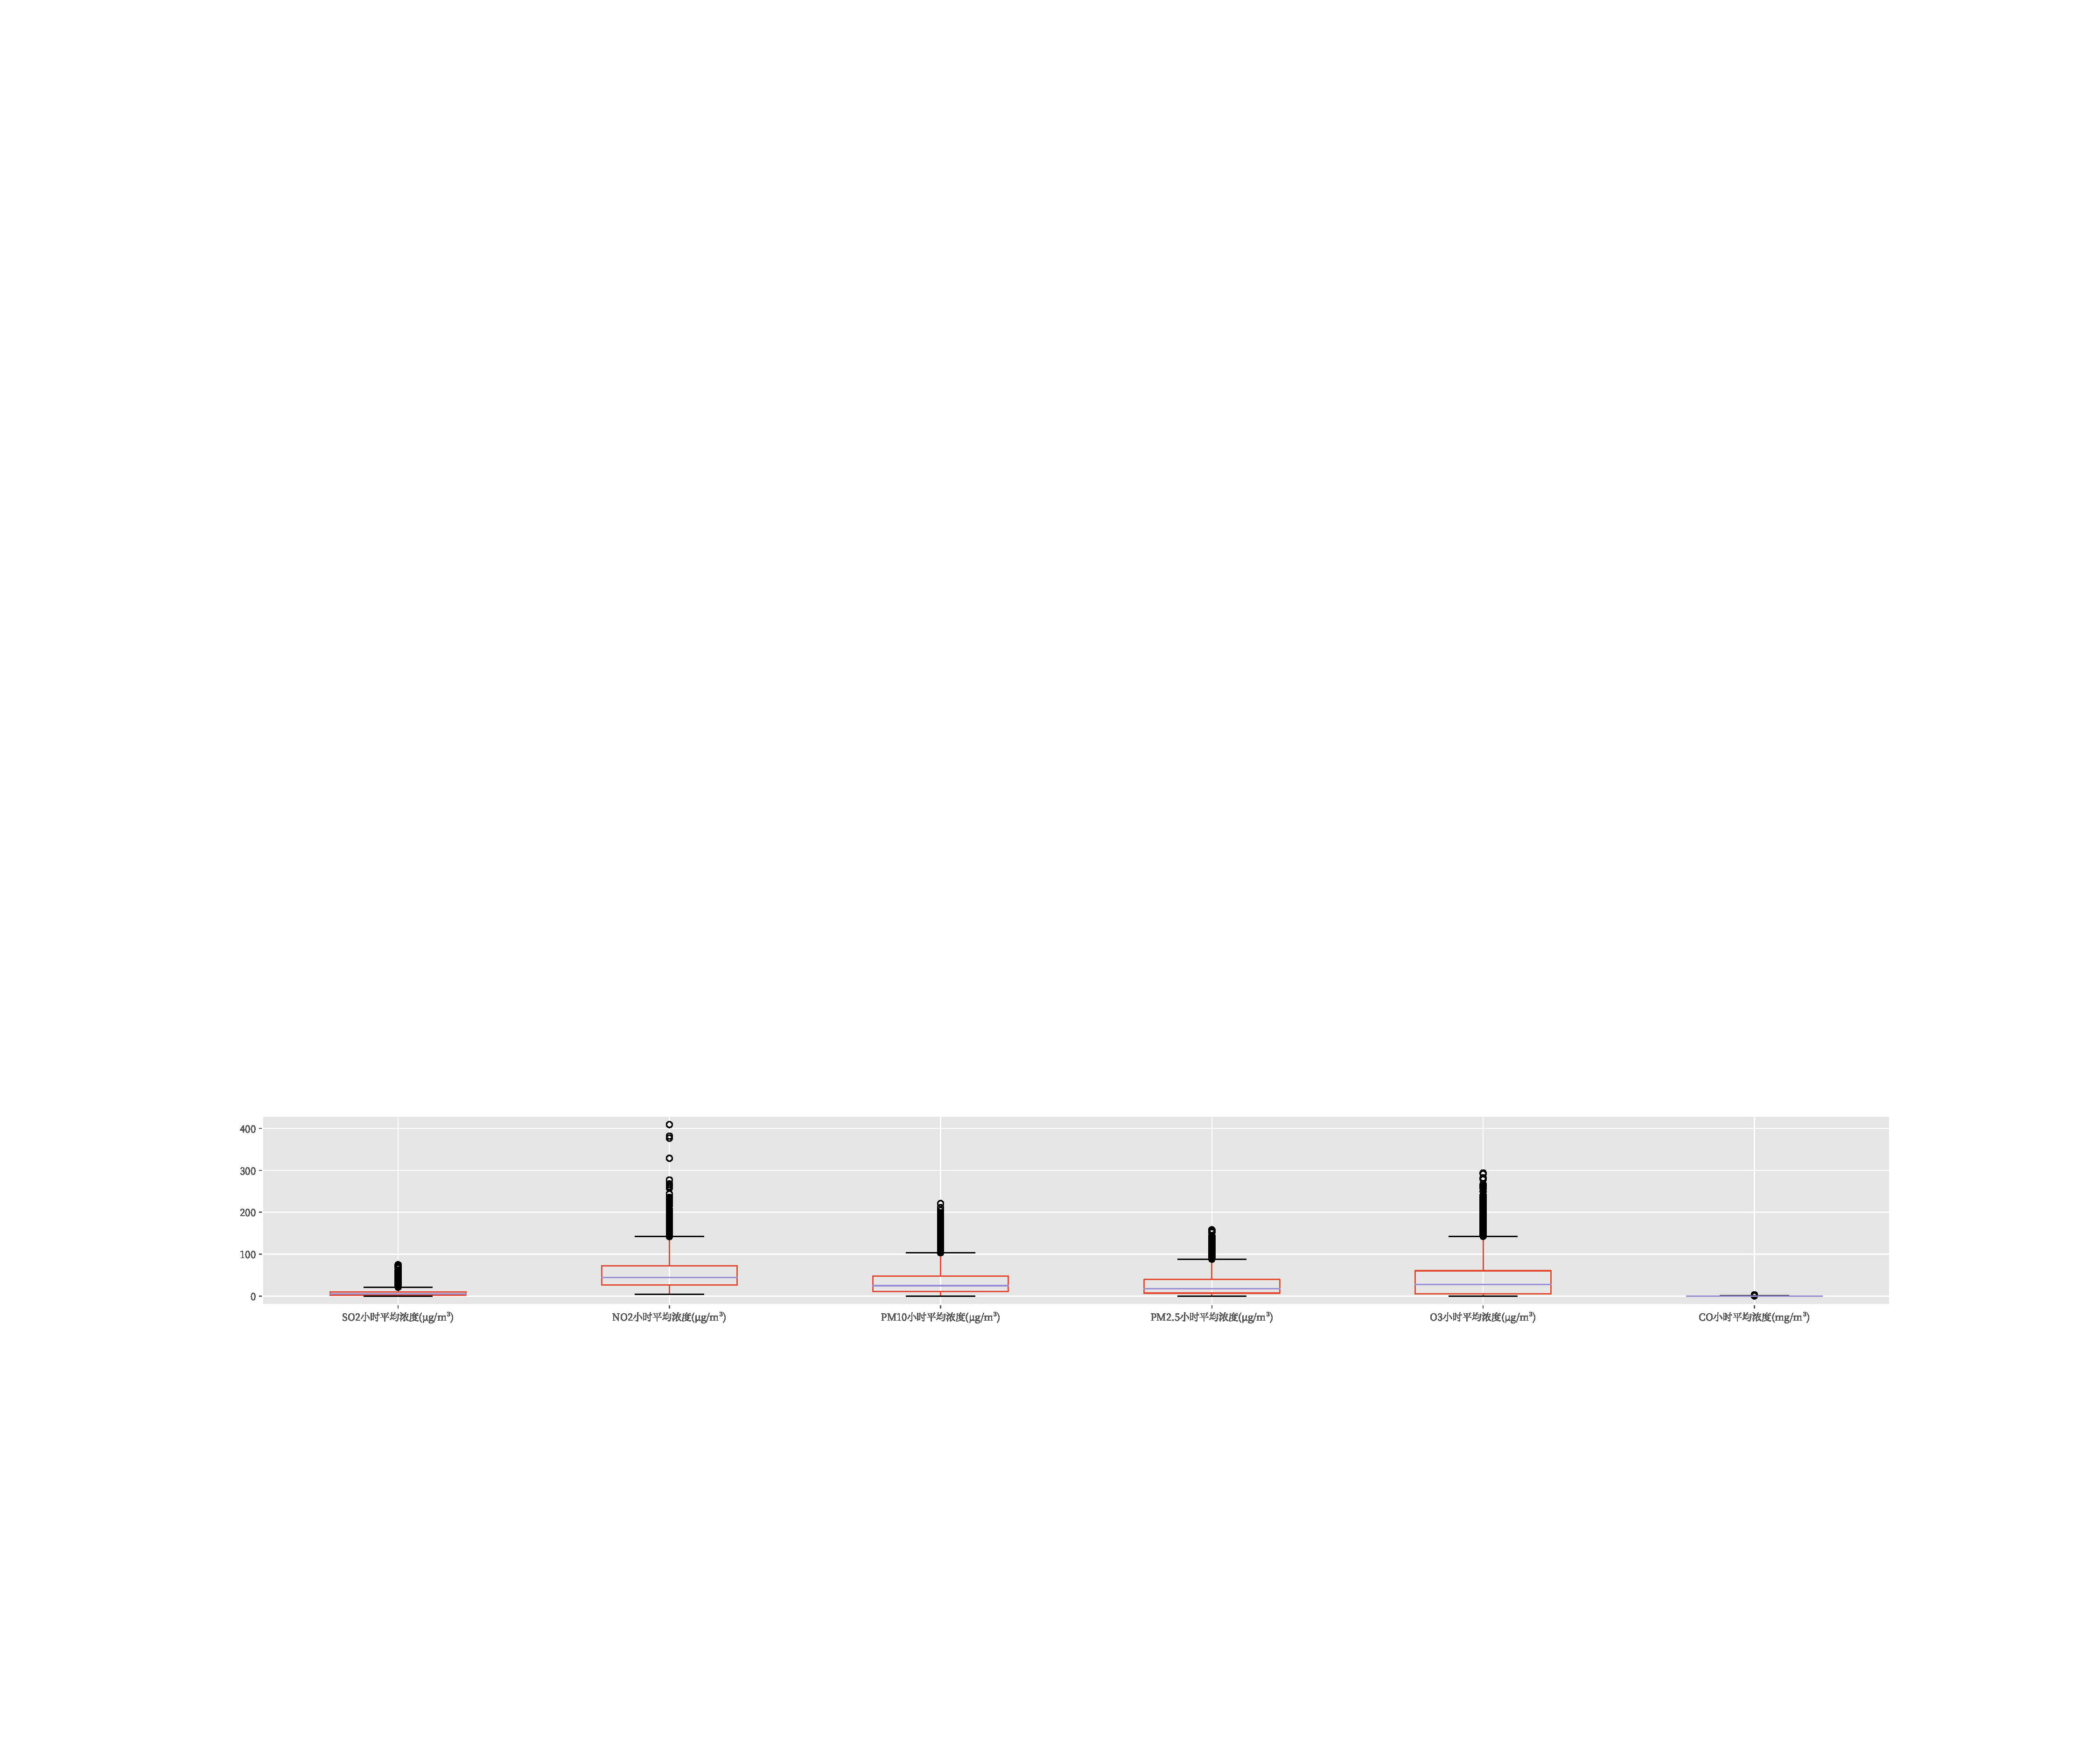
\includegraphics[width=1\textwidth]{box_plot_for_A2.pdf}\\
  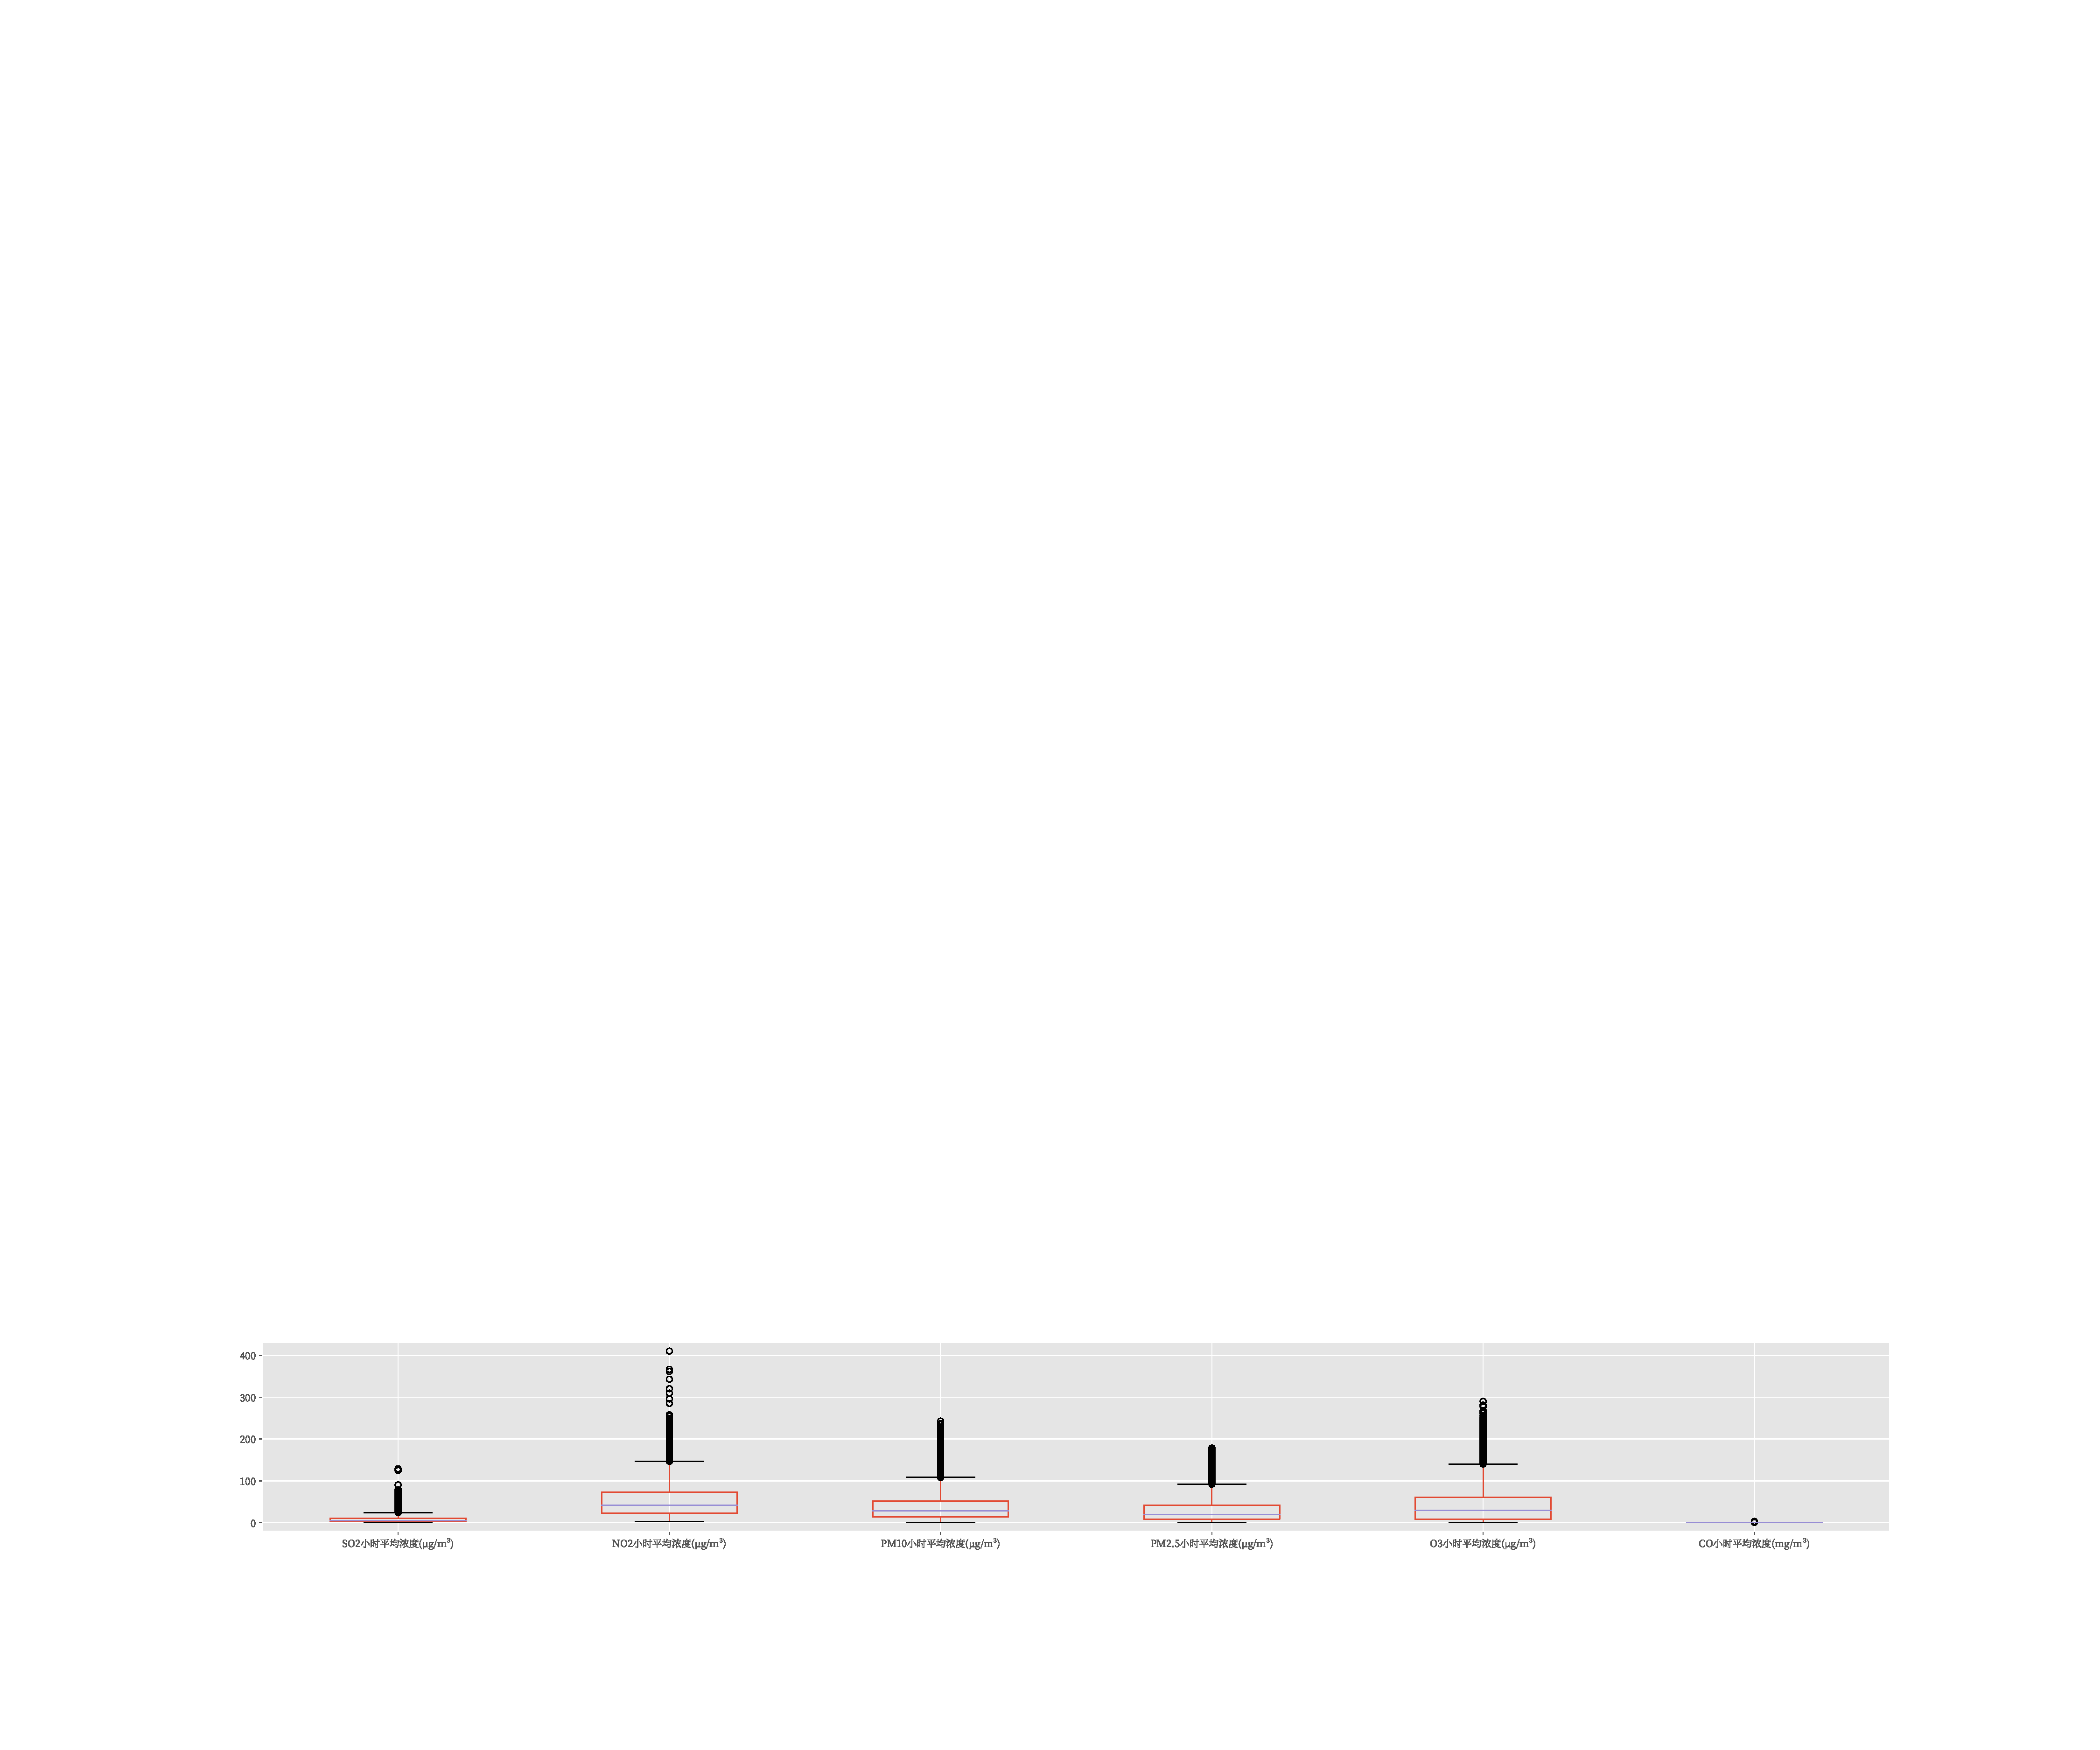
\includegraphics[width=1\textwidth]{box_plot_for_A3.pdf}\\
  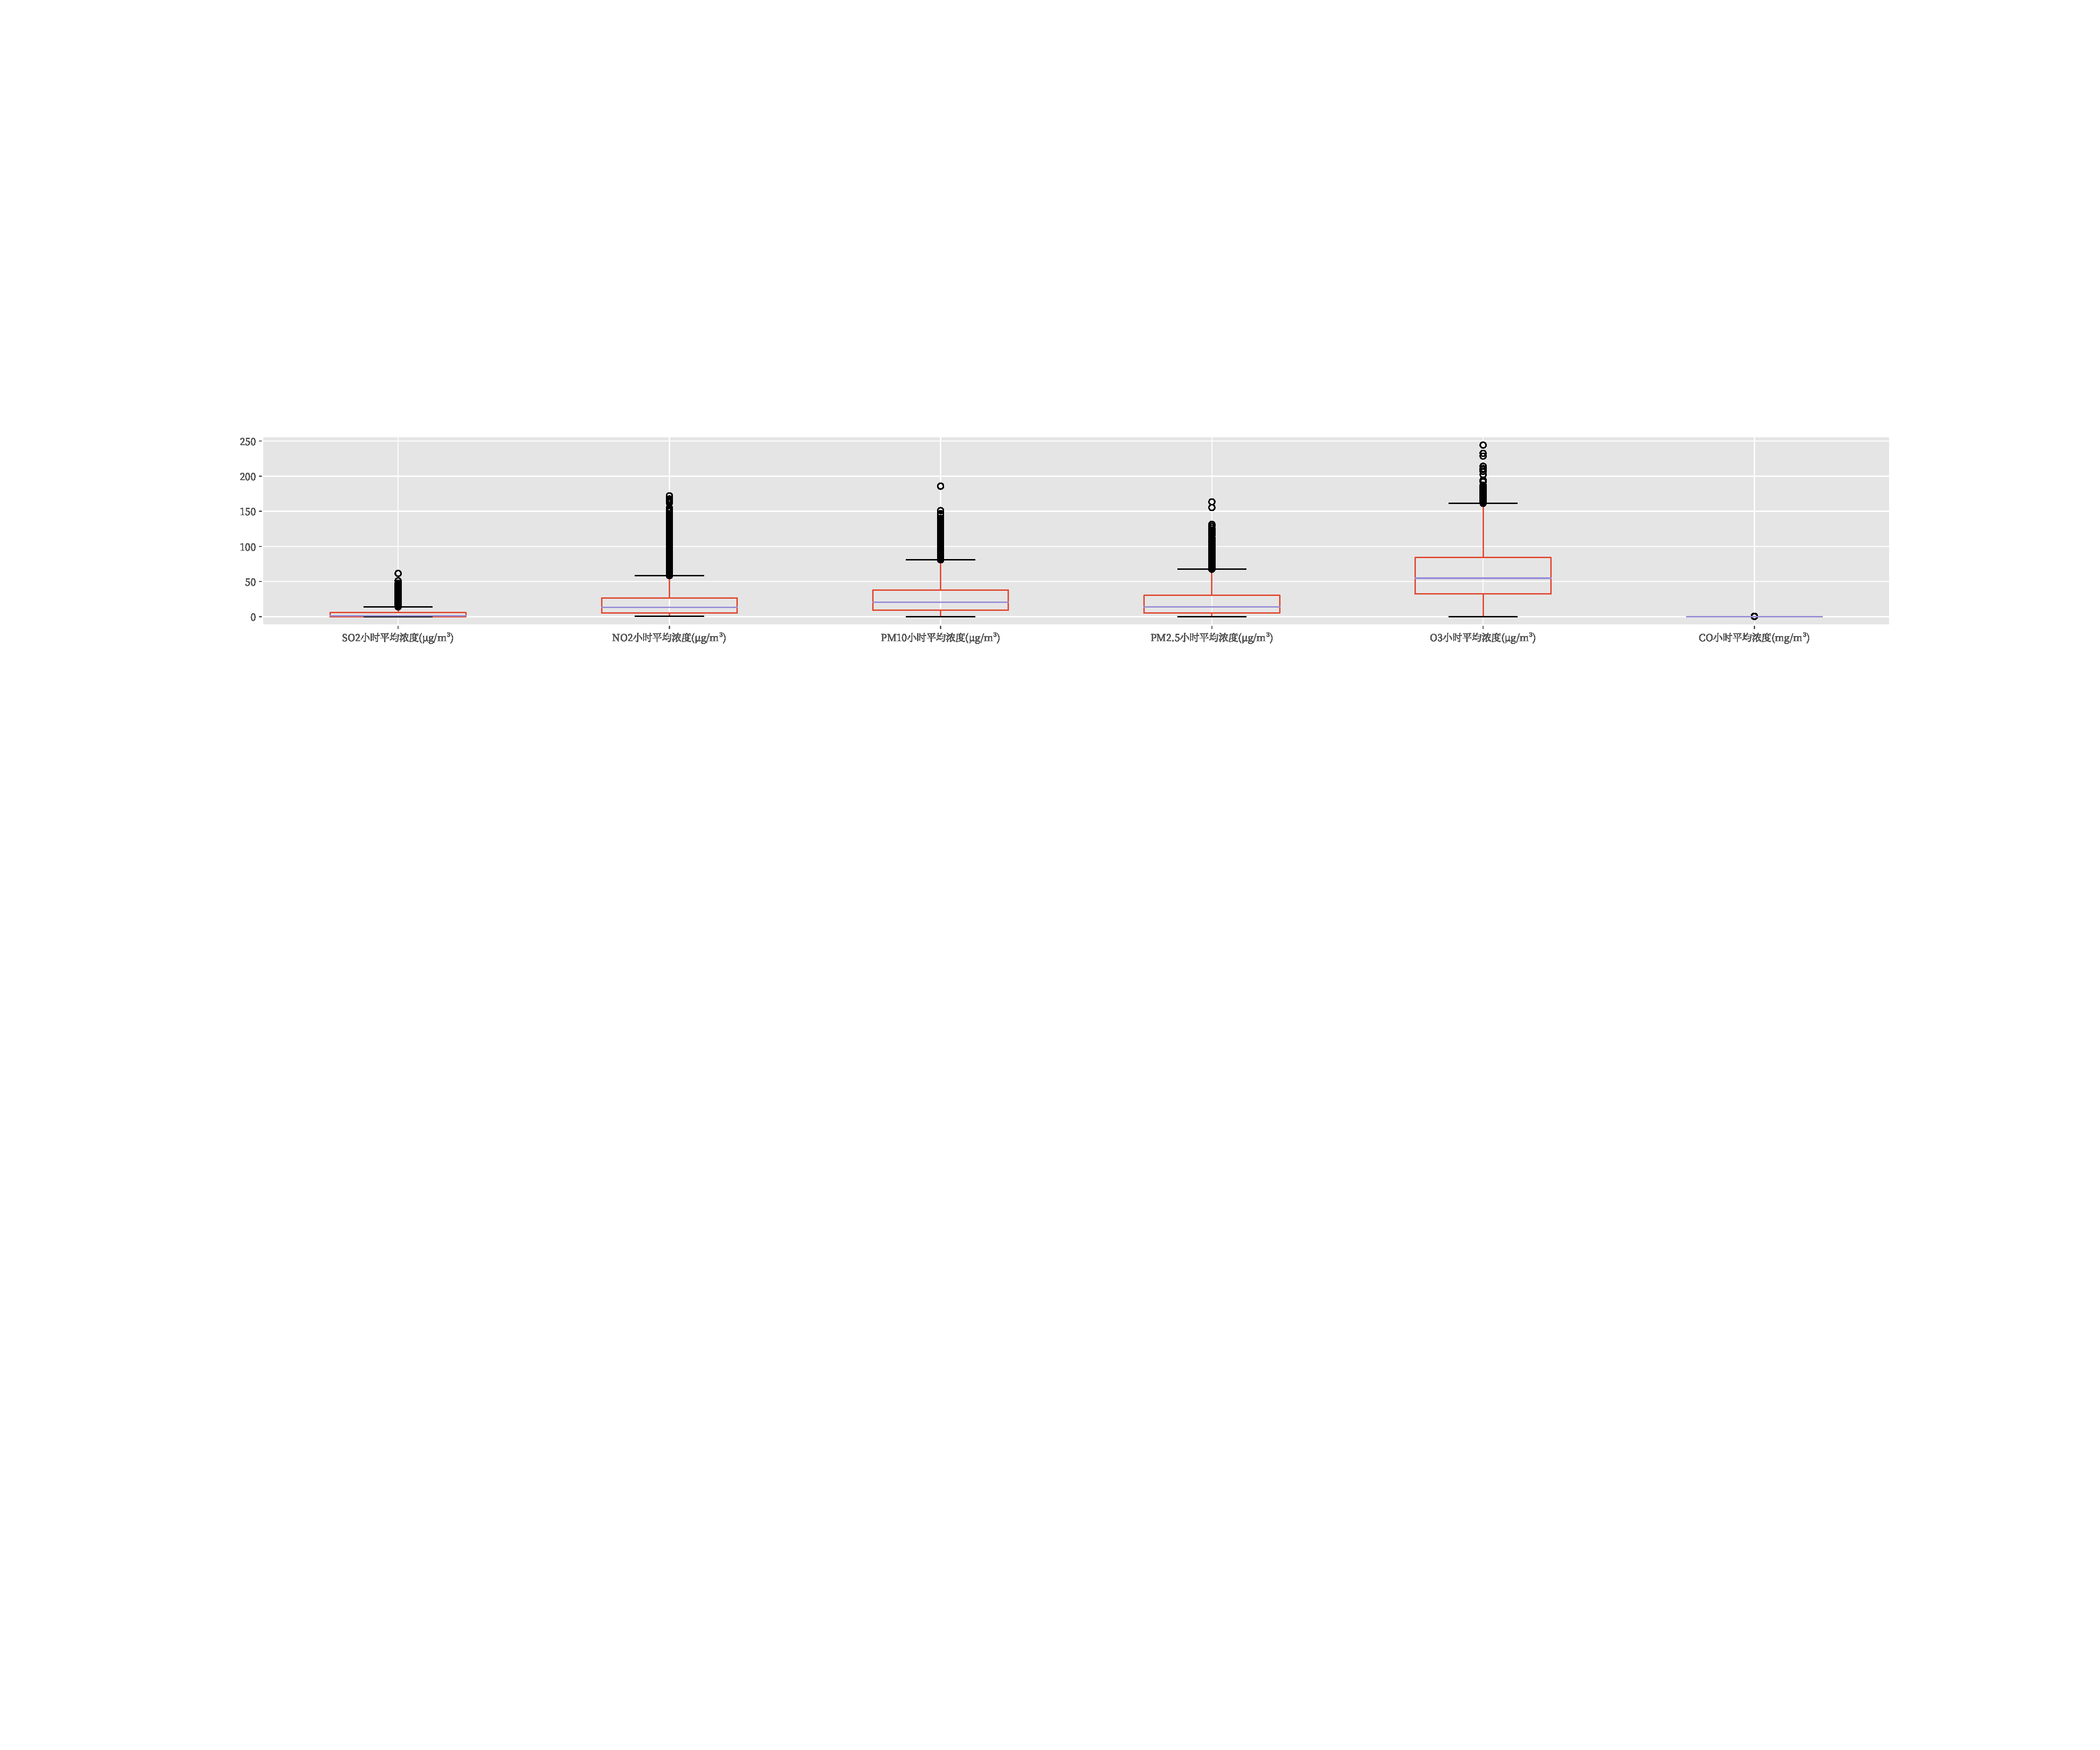
\includegraphics[width=1\textwidth]{box_plot_for_B.pdf}\\
  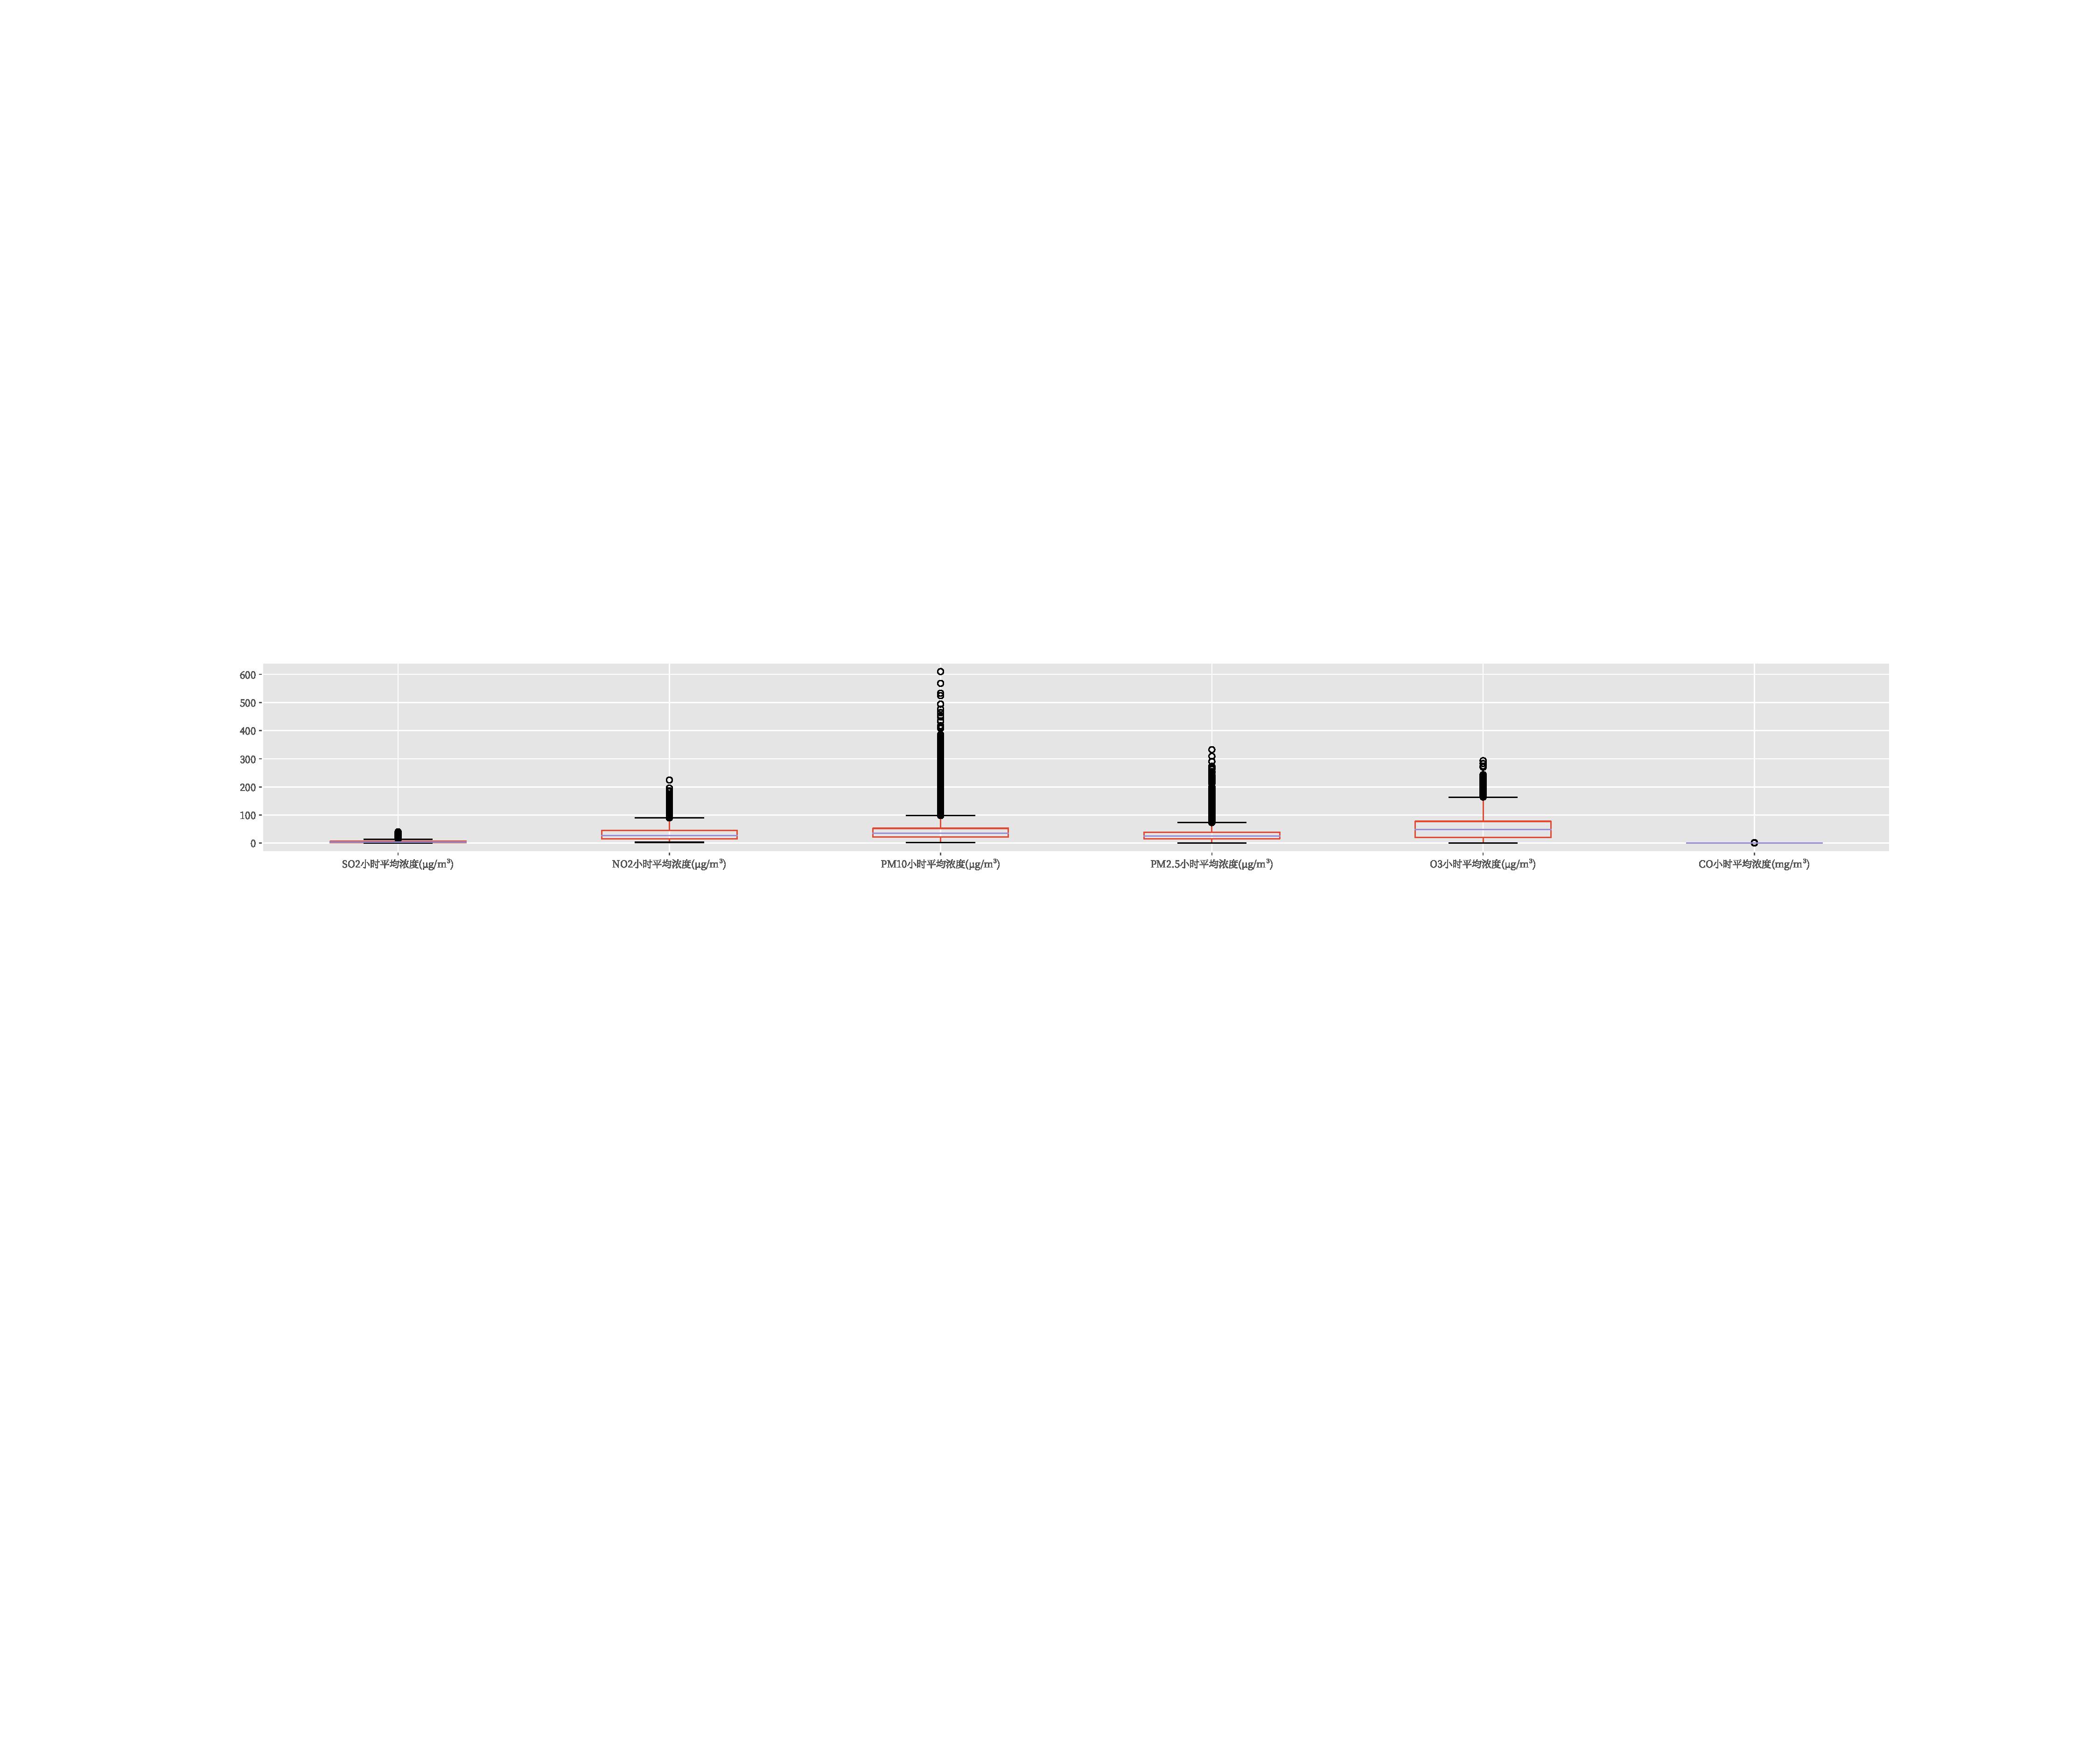
\includegraphics[width=1\textwidth]{box_plot_for_C.pdf}
  }
  \caption{数据异常值量化图}\label{fig_异常值}
\end{figure}


纠正由缺失数据导致的结论偏倚,缺失数据处理方法相继被提出。通过距离测量来识别相邻点,并通过相邻点观测值的完整值来估计缺失值的方法是一种常见的插补方法,如K近邻(K-Nearest Neighbor, KNN)算法\textsuperscript{\cite{ref3}}。这种插值方法虽然有效快速,但针对时序问题时,利用距离信息进行插补的方法则显得捉襟见肘。本文是一个预测空气质量的问题,与时间息息相关,因此本文采用了基于\textbf{半参数插值网络方法}\textsuperscript{\cite{ref4}},这种插值方法允许在插值阶段跨多元时间序列的多个纬度共享信息。

半参数插值网络模型如图\ref{fig_插值网络}所示,网络第一层是对D个时间序列中的每一个序列分别执行三个半参数单变量变换,每个变换都是基于径向基函数(Radial Basis Function, RBF),用以适应连续的时间观测。这三个变换分别是一个低通(平滑)插值函数${\varphi_d}$,一个高通(非平滑)插值函数${\delta_d}$以及一个强度函数${\tau_d}$。三个转换在时间点${r_k}$处的计算公式如下所示:

\begin{equation}
  M(c,\textbf{t},\varphi)=\sum_{t\in \textbf{t}}g(c,t,\varphi), \quad g(c,t,\varphi )=exp(-\varphi (c-t)^2) 
\end{equation}

\begin{equation}
  \tau_{ad} = f_\theta^\tau (c_a, \textbf{t}_d, \textbf{p}_d) = M(c_a, \textbf{t}_d,\varphi_d)
\end{equation}

\begin{equation}
  \epsilon_{ad} = f_\theta^\epsilon (c_a, \textbf{t}_d, \textbf{p}_d) = \frac{1}{M(c_a,\textbf{t}_d, \varphi _d)}\sum_{j = 1}^{L_{dn}}g(c_a, t_{jd},\varphi _d)p_{jd}  
\end{equation}

\begin{equation}
  \delta_{ad} = f_\theta^\delta(r_a.\textbf{t}_d,\textbf{p}_d)=\frac{1}{M(r_a,\textbf{t}_d,k\varphi_d)}\sum_{j = 1}^{L_{dn}}g(c_a,t_{jd},a\varphi_d)p_{jd}  
\end{equation}

其中,${L_{dn}}$为时间序列中总的观测数,${t_d}$表示第d维的时间序列,${\varepsilon_d}$采用的是参数为${\varphi_d}$平方指数核,${\delta_d}$采用的是参数为${a\varphi_d}$的平方指数核,其中${a>1}$。${\textbf{s}_d={t_d,p_d}}$是一个第n个数据案例的时间序列d的远足,${\textbf{t}_d={t_{1d},\dots,t_{L_{dn}}}}$是定义观测值的时间点列表,${\textbf{p}_d={p_{1d},\dots,p_{L_{dn}}}}$是相应的观测值列表。

第二层通过考虑所有时间序列的可学习相关性${\gamma_{dd^{'}}}$,合并每个参考时间点的所有D个时间序列的信息,即对每个d维的输入序列插入一个交叉维度插值${\lambda_d}$。此外,本文为每个输入维度d定义了一个瞬态分量${\sigma_d}$,该值为第一层高通插值${\delta_d}$与平滑交叉维度插值${\lambda_d}$之间的差值,计算公式如下:

\begin{equation}
  \lambda_{ad} = f_{\theta}^\lambda(c_a, \textbf{s}) = \frac{\sum_{d^{'}}\gamma_{dd^{'}}\beta_{ad^{'}}\epsilon_{ad^{'}}}{\sum_{d^{'}}\beta_{ad^{'}}}, \quad \sigma_{ad} = f_{\theta}^\sigma(c_a,\textbf{s}) = \delta_{ad}-\lambda _{ad} 
\end{equation}

我们使用平滑交叉维度插值${\lambda_d}$来获取平滑的趋势,瞬态分量${\sigma_d}$来捕获瞬态,强度函数${\tau_d}$来捕获关于观测及时发生的信息。插值后的部分结果如下图所示。{\color{red}[此处需要插图!!]}


% 图
\begin{figure}[htbp]
    \center{
    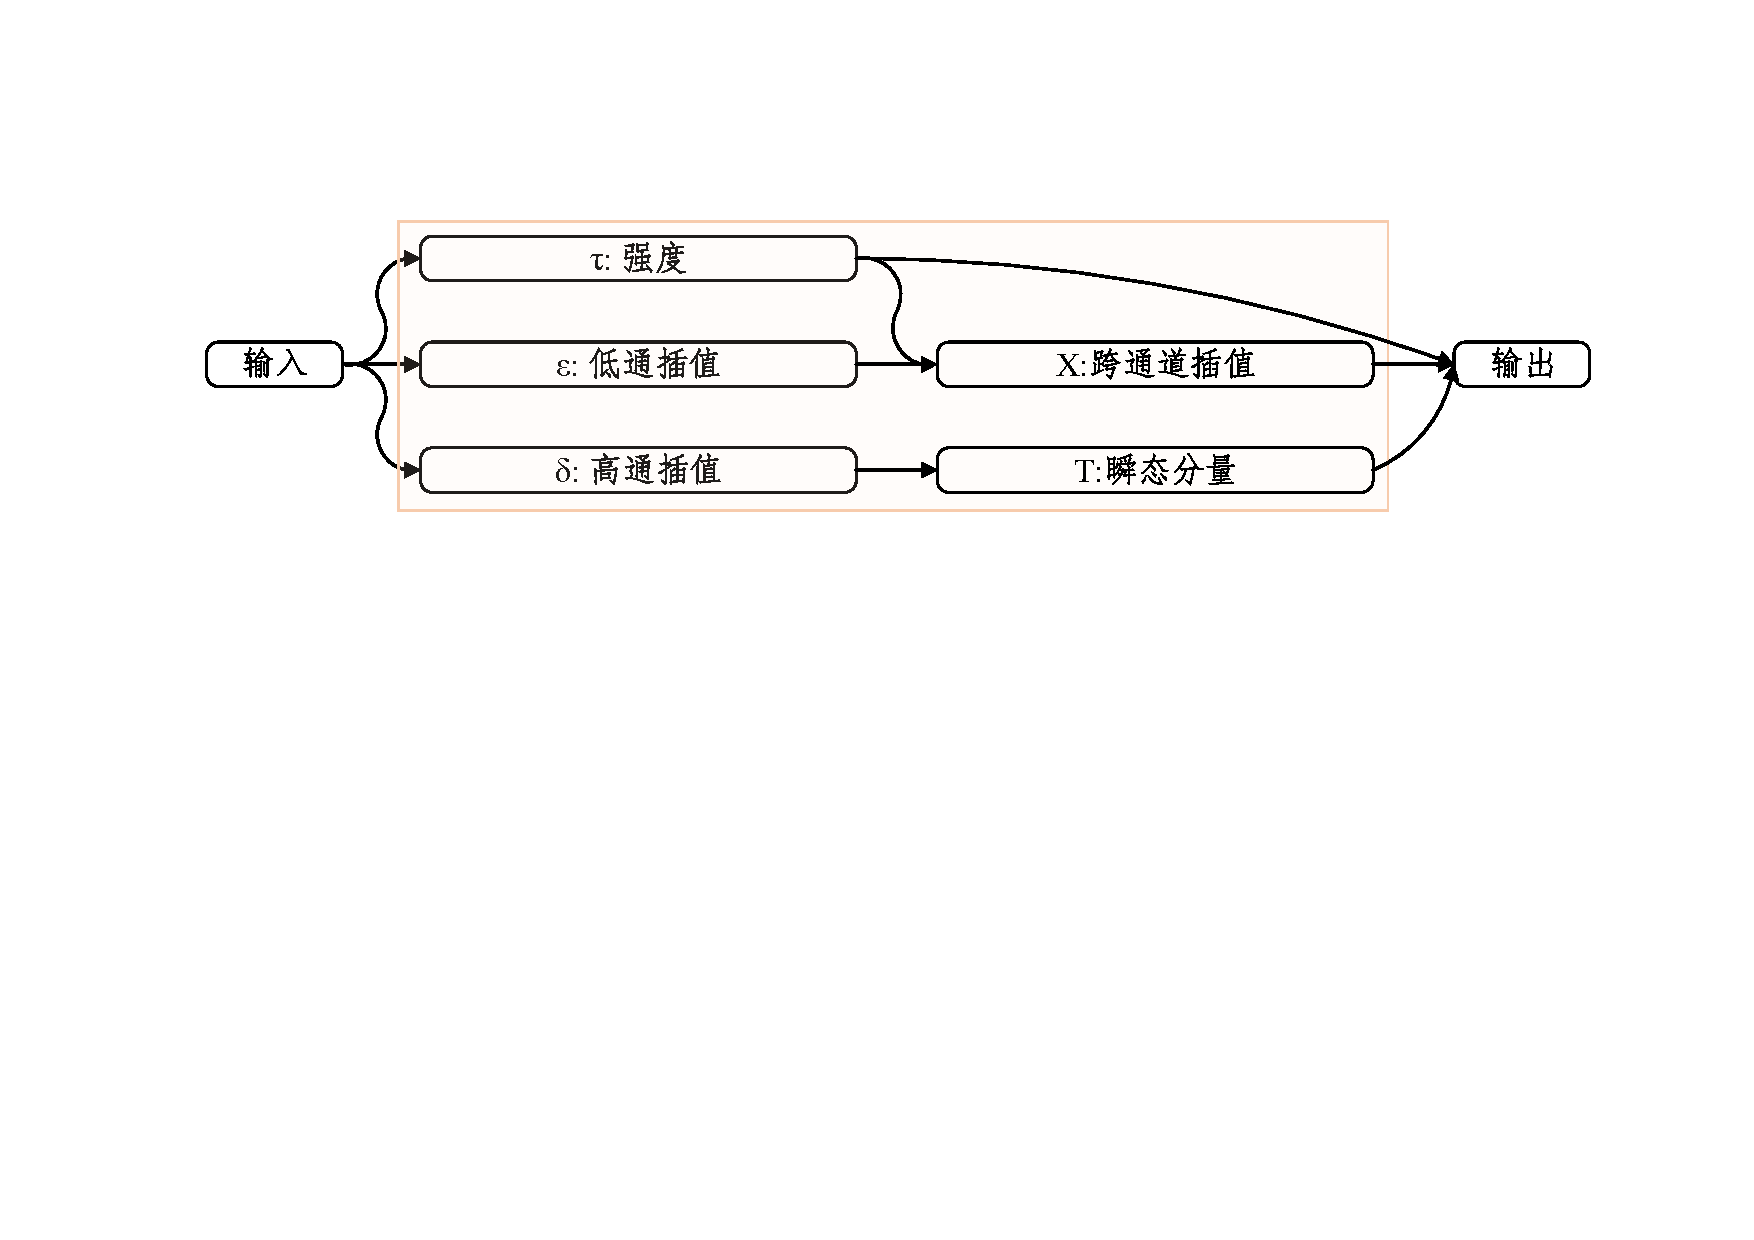
\includegraphics[width=.9\textwidth]{InterNet.pdf}
    }
    \caption{插值网络}\label{fig_插值网络}
\end{figure}

% 首先将时间

% 所给数据是时序数据,进行数据分析后,发现现有数据有较多的异常值。
% 包括空值,以及一些异常值,如臭氧浓度出现负值。
% % TODO: 数据分析, 图标, 数据缺失情况

% 对异常值的处理,常用的处理方式有删除和补值两种方法。
% 我们对不同的处理方法进行了分析。
% 1. 删除
% 简单删除是对异常值处理的最原始的方法,但是在多属性数据的情况下,容易造成数据的信息丢失。
% 2. 可能值填补异常值
% 用最可能的值来填补异常值的方式,要比直接全部删除不完全样本所丢失的信息要少。

% (1) 中位数填补
% 利用全体数据的中位数对异常值进行填补。
% (2) 均值填补
% 利用全体数据的均值对异常值进行填补。

% 分析所给数据,发现数据是时序的。
% 以均值为例,如果以全体数据做均值,然后填补异常值,可能会造成新填入数据成为新的异常值。% 放入例子, 图片

\subsection{模型求解和分析}
对数据清洗完毕后,按照附录中的AQI计算方法可以测出监测点A从2020年8月25日到8月28日每天实测的AQI和首要污染物。在计算AQI之前需要计算各项污染物的空气质量分指数(IAQI),其计算公式如下:

% 公式5.1
\begin{equation}
    IAQI_P = \frac{IAQI_{Hi}-IAQI_{LO}}{BP_{Hi}-BP_{LO}}\cdot(C_P-BP_LO)+IAQI_{LO}
\end{equation}

其中,${IAQI_P}$表示污染物P的空气质量分指数,${C_P}$表示污染物P的质量浓度值,${BP_{Hi}}$和${BP_{LO}}$表示与${C_P}$相近的污染物浓度限值的高位值与低位值,${IAQI_{Hi}}$和${IAQI_{LO}}$表示与${BP_{Hi}}$、${BP_{LO}}$对应的空气质量分数。各项污染物项目浓度限值及对应的空气质量分指数级别如表\ref{tab1}所示。

% 表1
% Table generated by Excel2LaTeX from sheet 'Sheet2'
\begin{table}[htbp]
    \centering
    \caption{IAQI及对应的污染物浓度限值}\label{tab1}%
    \begin{threeparttable}
      \begin{tabular}{p{9em}ccccccccc}
      \toprule
      指数或污染物项目 & \multicolumn{8}{p{32.44em}}{IAQI及对应的污染物浓度限值}                & \multicolumn{1}{p{4.055em}}{单位} \\
      \midrule
      IAQI  & 0     & 50    & 100   & 150   & 200   & 300   & 400   & 500   & \multicolumn{1}{p{4.055em}}{-} \\
      ${CO}$24小时平均 & 0     & 2     & 4     & 14    & 24    & 36    & 48    & 60    & \multicolumn{1}{p{4.055em}}{${mg/m^3}$} \\
      ${SO_2}$24小时平均 & 0     & 50    & 150   & 475   & 800   & 1600  & 2100  & 2620  & \multicolumn{1}{c}{\multirow{7}[1]{*}{${\mu g/m^3}$}} \\
      ${NO_2}$24小时平均 & 0     & 40    & 80    & 180   & 280   & 565   & 750   & 940   &  \\
      O3-Max8h & 0     & 100   & 160   & 215   & 265   & 800   & \multicolumn{1}{p{4.055em}}{-} & \multicolumn{1}{p{4.055em}}{-} &  \\
      粒径小于等于10 & \multirow{2}[0]{*}{0} & \multirow{2}[0]{*}{50} & \multirow{2}[0]{*}{150} & \multirow{2}[0]{*}{250} & \multirow{2}[0]{*}{350} & \multirow{2}[0]{*}{420} & \multirow{2}[0]{*}{500} & \multirow{2}[0]{*}{600} &  \\
      ${PM_10}$24小时平均 &       &       &       &       &       &       &       &       &  \\
      粒径小于等于2.5 & \multirow{2}[1]{*}{0} & \multirow{2}[1]{*}{35} & \multirow{2}[1]{*}{75} & \multirow{2}[1]{*}{115} & \multirow{2}[1]{*}{150} & \multirow{2}[1]{*}{250} & \multirow{2}[1]{*}{350} & \multirow{2}[1]{*}{500} &  \\
      ${PM2.5}$24小时平均 &       &       &       &       &       &       &       &       &  \\
      \bottomrule
      \end{tabular}%
      \begin{tablenotes}%表格注释
      \item[1]\scriptsize{ 臭氧(${O_3}$)最大8小时滑动平均浓度值高于800${\mu g∕m^3}$的,不再进行其空气质量分指数计算。} 
      \item[2]\scriptsize{ 其余污染物浓度高于IAQI=500对应限值时,不再进行其空气质量分指数计算。} 
      \end{tablenotes}
    \end{threeparttable}
  \end{table}%
  
在计算完单个IAQI之后,空气质量指数(AQI)取各分指数中的最大值,即空气质量等级范围根据AQI数值划分,等级对应的AQI范围如表\ref{tab2}所示。

% 公式5.2
\begin{equation}
  AQI = max{IAQI_{SO_2},IAQI_{NO_2},IAQI_{PM_10},IAQI_{PM_2.5},IAQI_{O_3},IAQI_{CO}}
\end{equation}

其中${IAQI_{SO_2},IAQI_{NO_2},IAQI_{PM_10},IAQI_{PM_2.5},IAQI_{O_3},IAQI_{CO}}$为各污染物的分指数,

% 表2
  % Table generated by Excel2LaTeX from sheet 'Sheet2'
\begin{table}[htbp]
    \centering
    \caption{空气质量等级及对应空气质量质数(AQI)范围}\label{tab2}%
      \begin{tabular}{p{11em}p{4.055em}p{4.055em}p{4.055em}p{4.055em}p{4.055em}p{4.055em}}
      \toprule
      空气质量等级 & 优     & 良     & 轻度污染  & 中度污染  & 重度污染  & 严重污染 \\
      \midrule
      空气质量指数(AQI)范围 & [0,50] & [51,100] & [101,150] & [151,200] & [201,300] & [301,+∞) \\
      \bottomrule
      \end{tabular}%
  \end{table}%

当AQI小于或等于50(即空气质量评价为“优”)时,称当天无首要污染物;当AQI大于50时,IAQI最大的污染物为首要污染物。若IAQI最大的污染物为两项或两项以上时,并列为首要污染物;IAQI大于100的污染物为超标污染物。

在完成数据预处理之后,经过IAQI的计算,得到了监测点A从2020年8月25日到8月28日每天实测的AQI和首要污染物,结果如表\ref{tab3}所示。从表中数据可以看出,监测的四天中只有2020年8月26日无首要污染物,其余三天的首要污染物均为${O_3}$。因为在计算当前结果时,没有考虑气象条件对污染物的影响(如风速对监测点A的污染物浓度的影响),也没有考虑二次污染的情况,所以从表中数据的AQI计算结果缺乏一定的真实性,需要在全面综合的考虑气象条件以及各污染物之间的相关性后重新计算,完成对空气质量的可靠估计。


% 表3
  % Table generated by Excel2LaTeX from sheet 'Sheet2'
\begin{table}[htbp]
    \centering
    \caption{AQI计算结果}\label{tab3}%
      \begin{tabular}{cccp{5em}}
      \toprule
      \multirow{2}[2]{*}{监测日期} & \multirow{2}[2]{*}{地点} & \multicolumn{2}{c}{AQI计算} \\
            &       & \multicolumn{1}{p{4.055em}}{AQI} & 首要污染物 \\
      \midrule
      2020/8/25 & 监测点A  & 60    & ${O_3}$ \\
      2020/8/26 & 监测点A  & 46    & 无 \\
      2020/8/27 & 监测点A  & 108   & ${O_3}$ \\
      2020/8/28 & 监测点A  & 137   & ${O_3}$ \\
      \bottomrule
      \end{tabular}%
  \end{table}%
  


%--------------------问题二的模型建立与求解----------------------
\section{问题二的模型建立与求解}
\subsection{问题二的描述分析}
问题二是在污染物排放情况不变的条件下,考虑气象条件。利用指定的数据,根据污染物对气象条件的影响程度,对气象条件进行合理分类,并对分类后的气象条件特性进行分析。针对这个问题,本文首先考虑到的是\textbf{时间滞后性问题},通过分析各气象条件与6项污染物之间的峰值,计算出了各影响因子之间的时间滞后性,为使得AQI的结果更加贴近实际的预测,我们将计算出的滞后时间进行了调整,使得各影响因子的峰值实现了跨时组合。

\subsection{时间滞后性的考虑}
空气质量指数受到多种气象条件的影响,而气象条件由于其本身特性,会导致AQI的变化产生一定的滞后性。
% 如,xx 点吹的风,在  时间后会在 AQI 上体现出来。% 具体时间依据图表。
% 下图, 风力的折线图。
% TODO: 风力对 AQI 的影响,时间滞后性。

\subsection{相关性分析}
\begin{figure}[htbp]
  \center{
  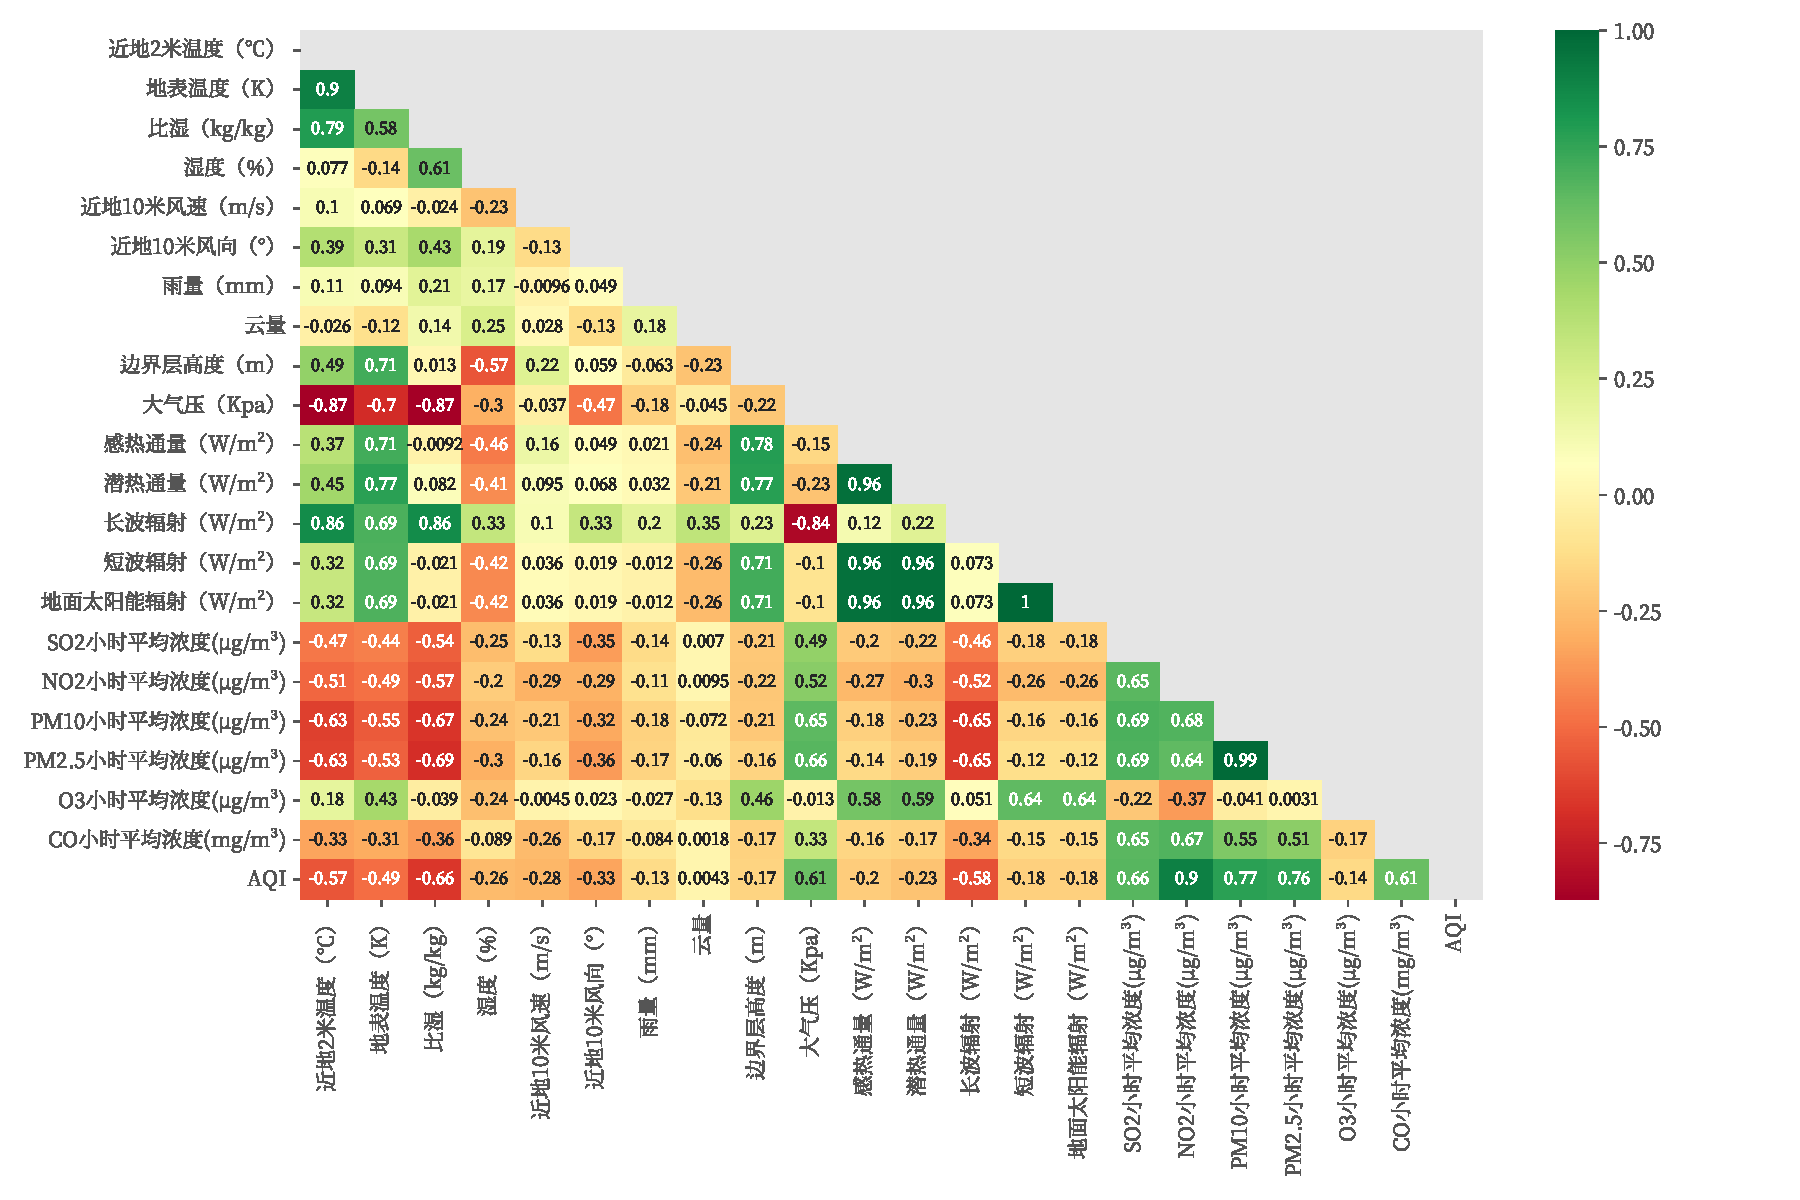
\includegraphics[width=.9\textwidth]{A-0相关性分析.pdf}
  }
  \caption{相关性分析}\label{fig_相关性分析}
\end{figure}

根据如图所示的相关系数热力图,可以直观地观察到,温度,湿度,风速,近地2米温度,地表温度,比湿,湿度,边界层高度,感热通量,潜热通量,短波辐射,地面太阳能辐射这12个指标与污染物浓度相关性较高。

\subsection{数学模型的建立}
常用聚类方法有K-Means(K 均值)聚类,用高斯混合模型(GMM)的最大期望(EM)聚类,谱聚类等等。

本题采用谱聚类方式。因为谱聚类相对于传统的K-Means算法, 谱聚类对数据分布的适应性更强,聚类效果也很优秀,同时聚类的计算量也小很多。

聚类结果如下图所示:

\begin{figure}[htbp]
    \center{
    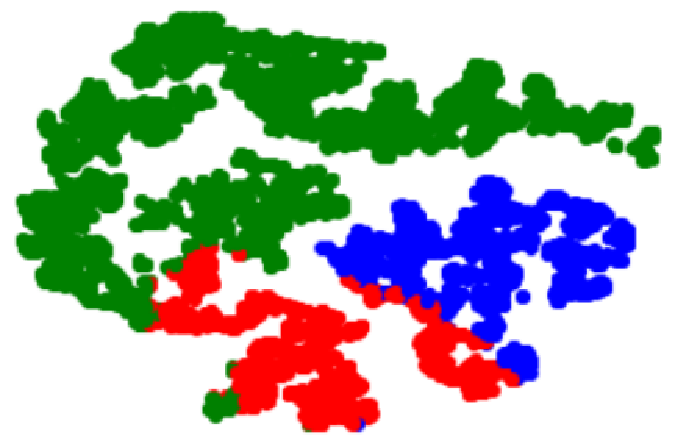
\includegraphics[width=.9\textwidth]{cluster.pdf}
    }
    \caption{聚类结果}\label{fig_聚类结果}
\end{figure}

簇中心气象指标:
\begin{figure}[htbp]
  \center{
  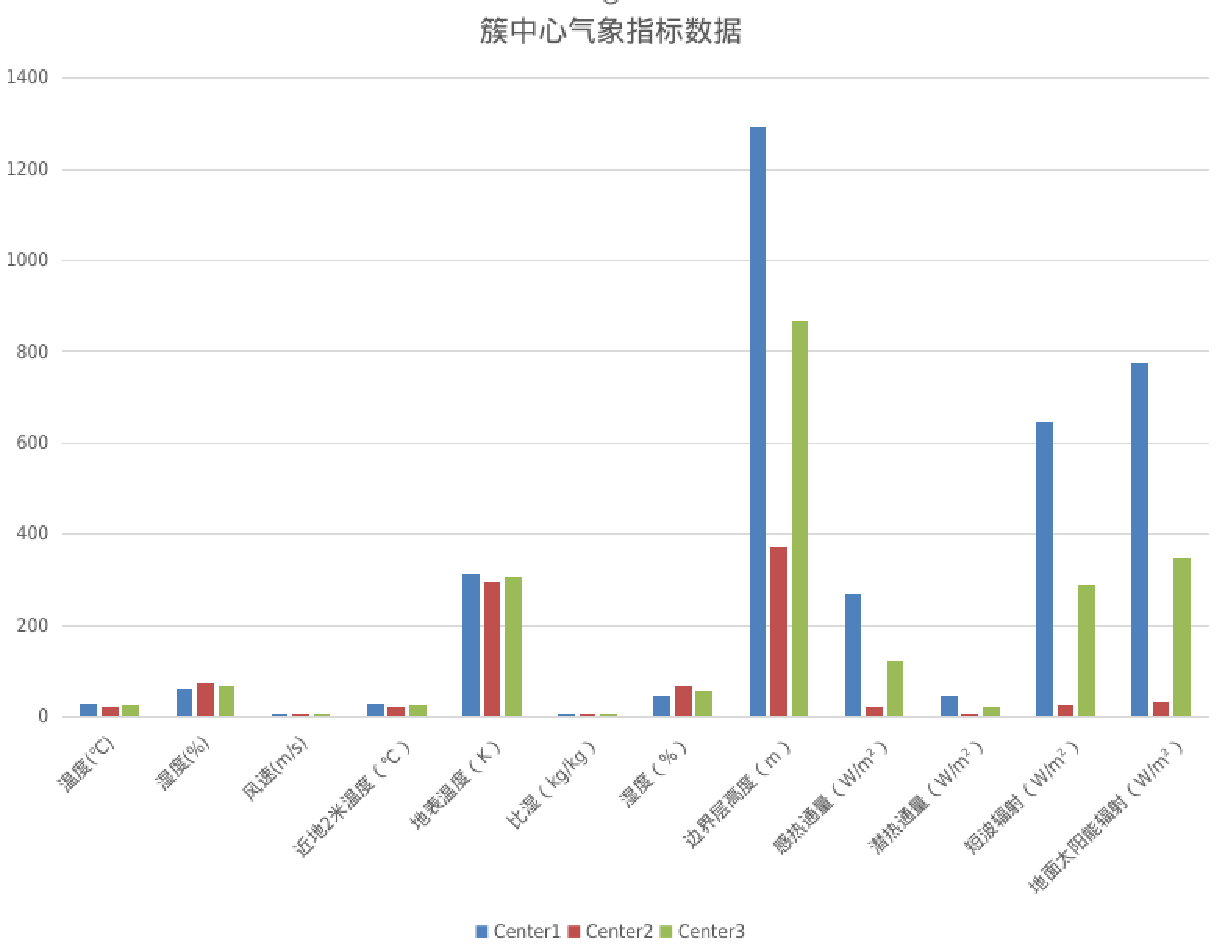
\includegraphics[width=.9\textwidth]{clustering-center.pdf}
  }
  \caption{簇中心气象指标}\label{簇中心气象指标}
\end{figure}

由聚类结果图和中心气象指标图示可知,分成三类:
一类气象条件, 湿度低但温度风速大
二类气象条件正好相反,温度低,湿度高,风速低
三类气象条件处于一类和二类之间,温度适中


\subsection{模型求解和分析}

% 图  
\begin{figure}[htbp]
  \center{
    \subfigure[pic1.]{
    \begin{minipage}[t]{0.25\linewidth}
    \centering
    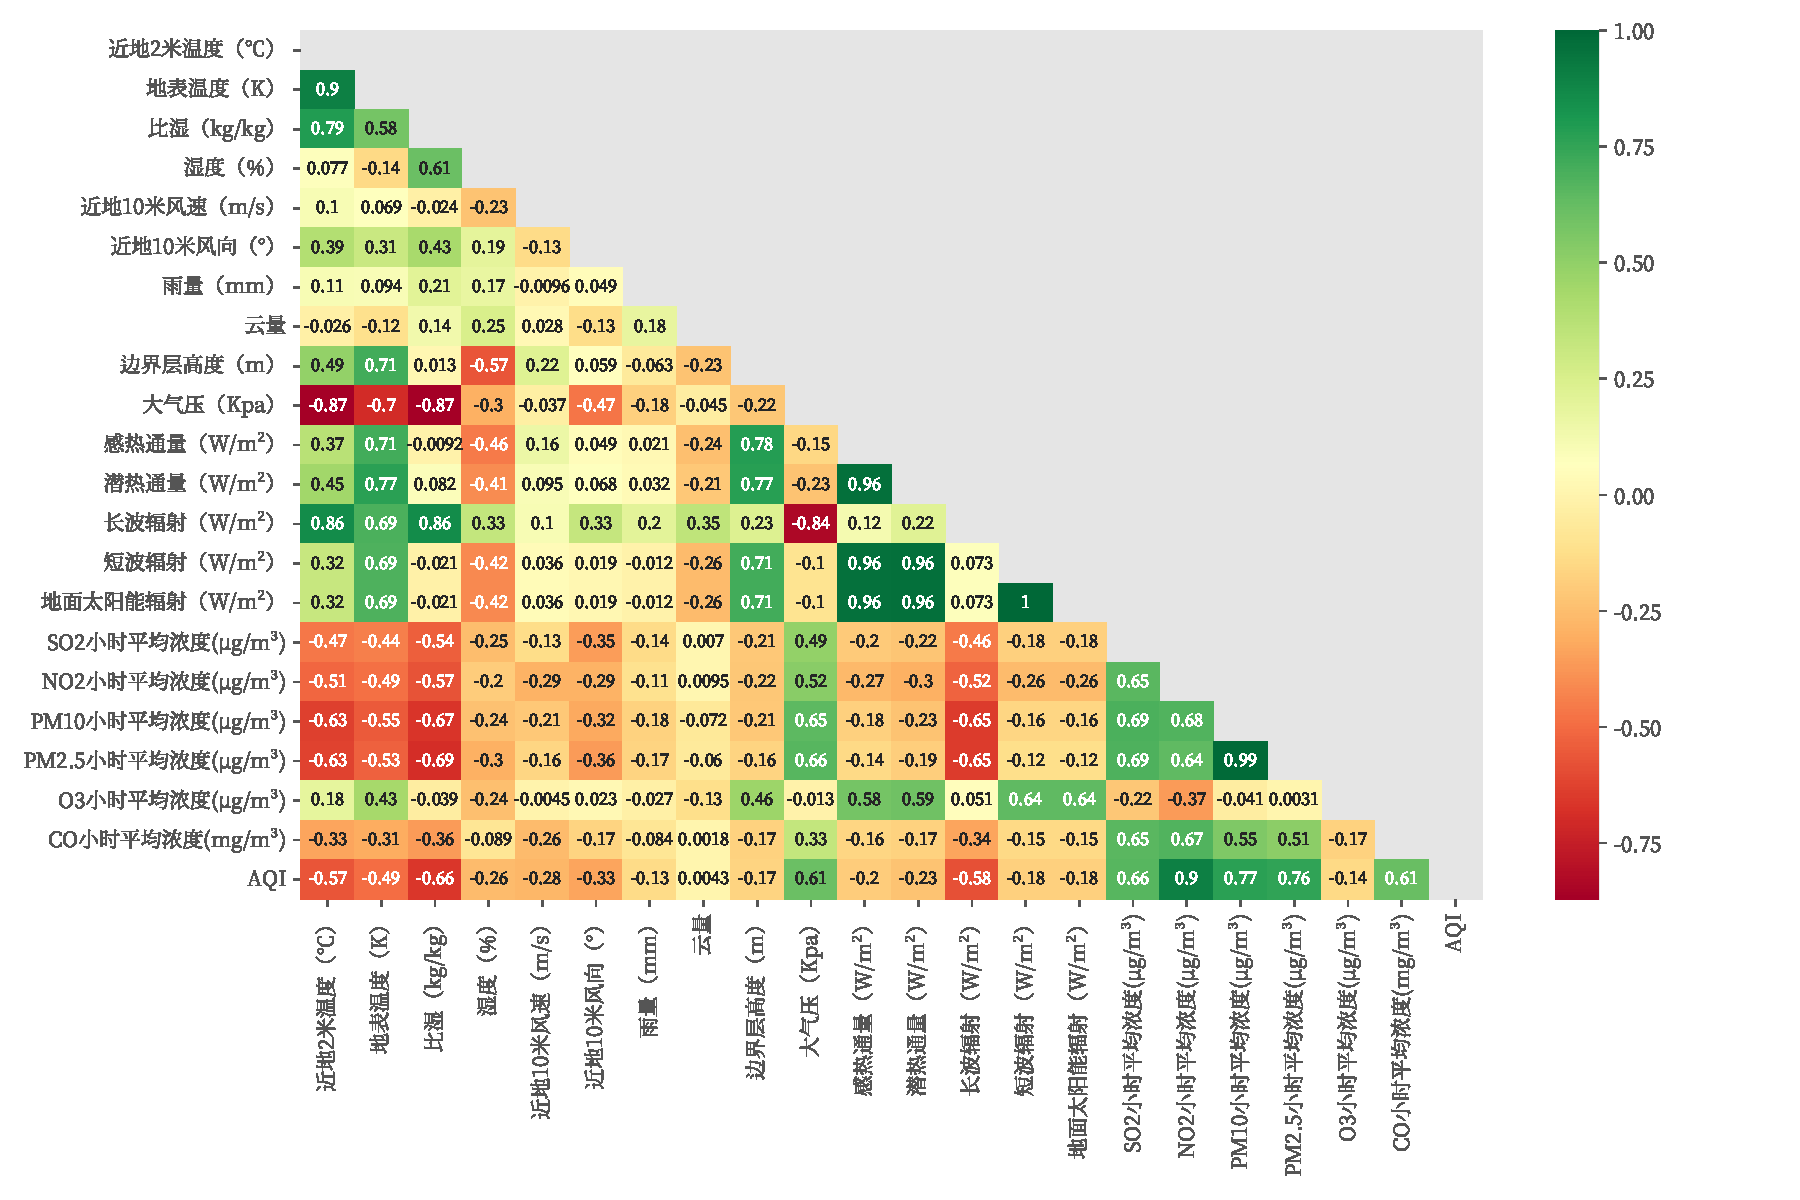
\includegraphics[width=5in]{A-0相关性分析.pdf} 
    \end{minipage}}

    \subfigure[pic2.]{
    \begin{minipage}[t]{0.25\linewidth}
    \centering
    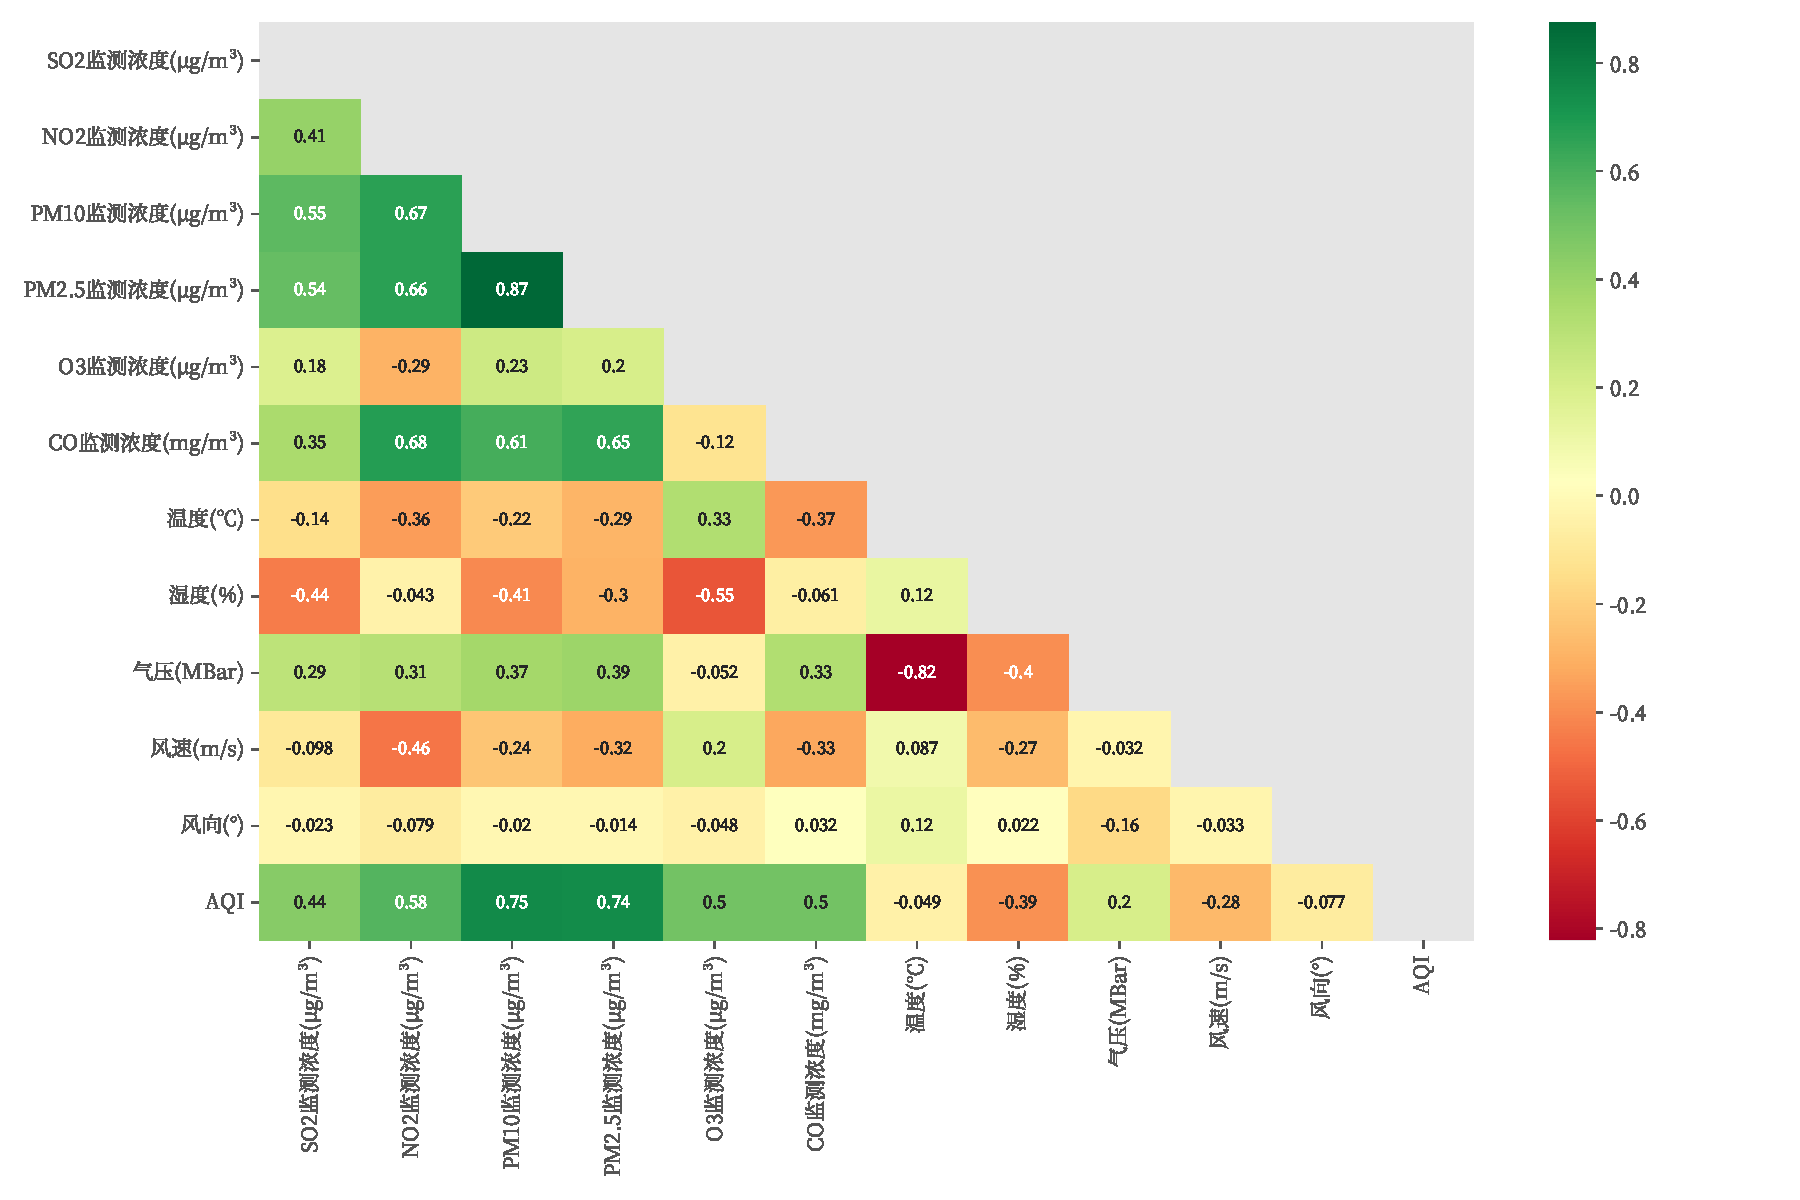
\includegraphics[width=5in]{A-1相关性分析.pdf} 
    \end{minipage}}

    \subfigure[pic3.]{
    \begin{minipage}[t]{0.25\linewidth}
    \centering
    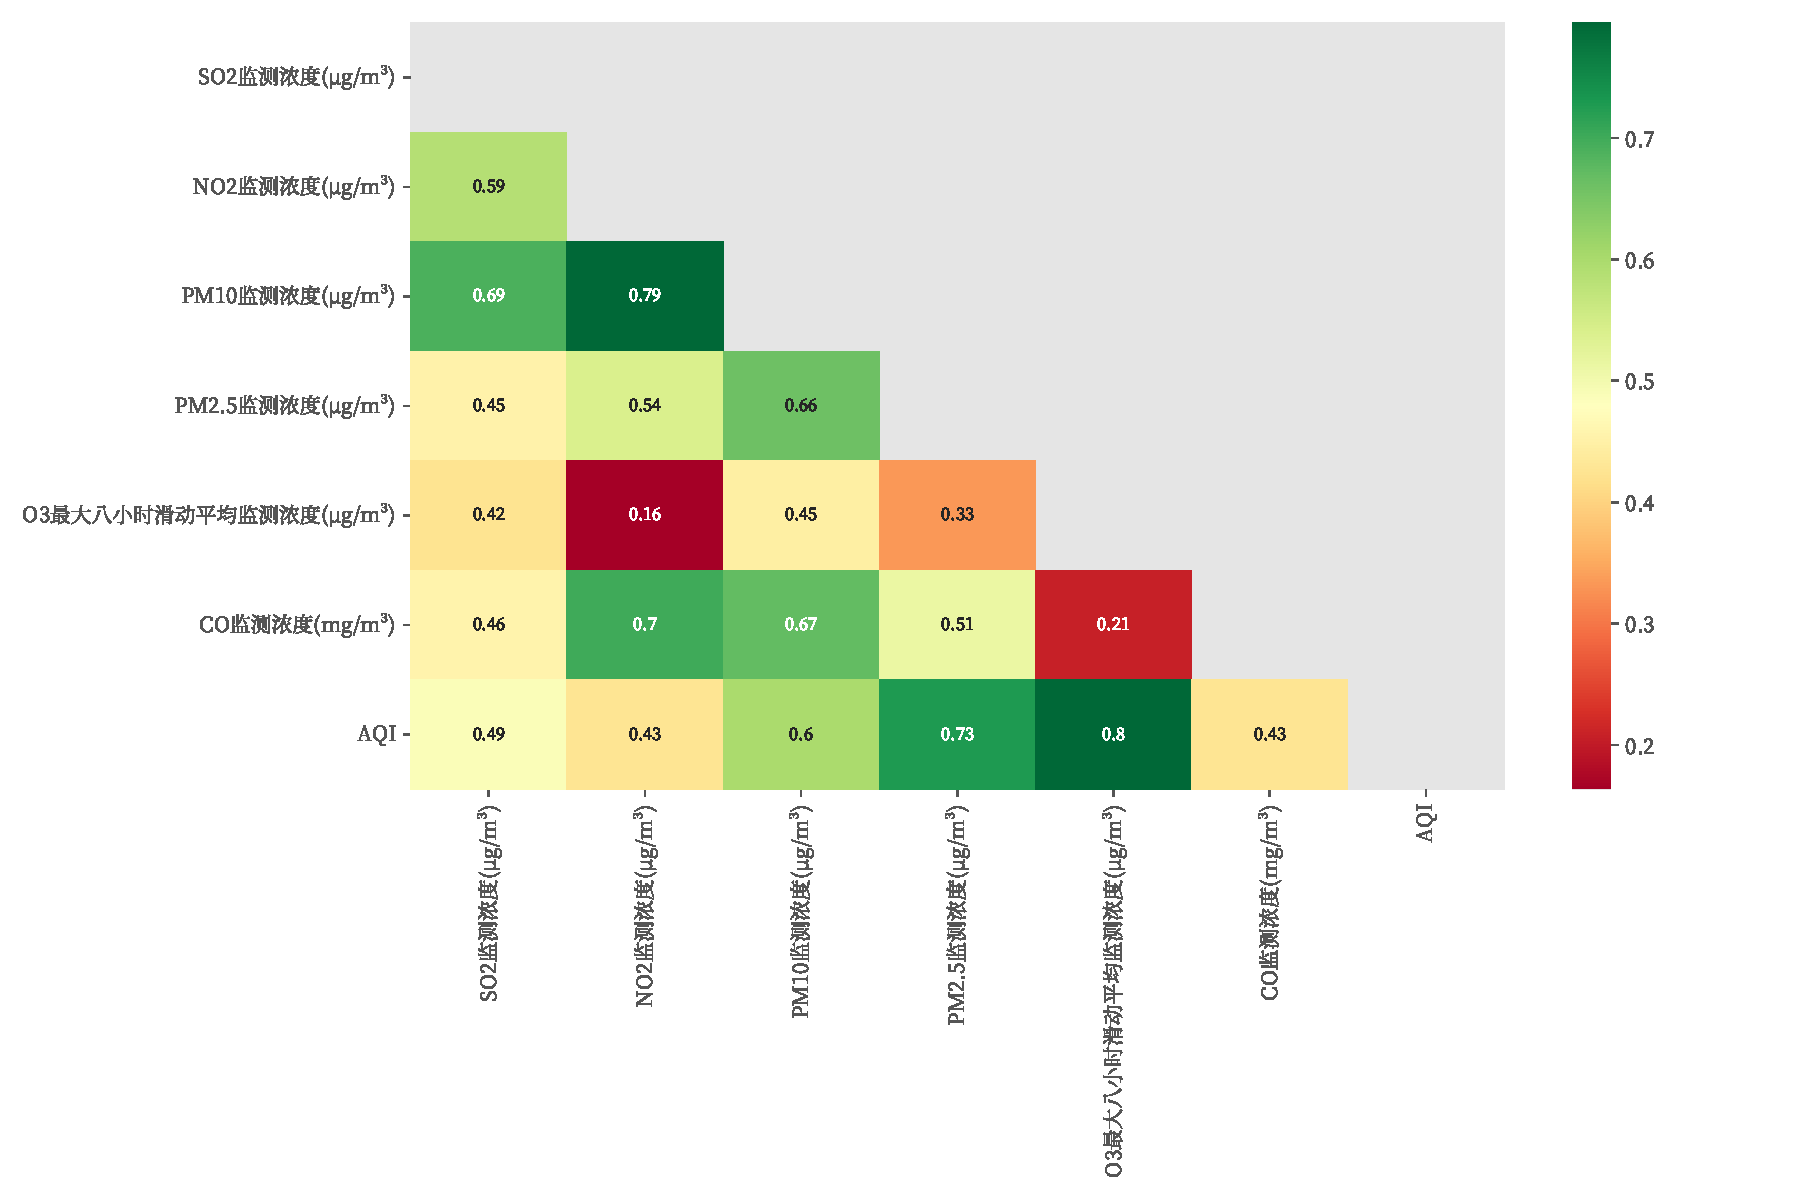
\includegraphics[width=5in]{A-2相关性分析.pdf}
    \end{minipage}}

    \subfigure[pic4.]{
    \begin{minipage}[t]{0.25\linewidth}
    \centering
    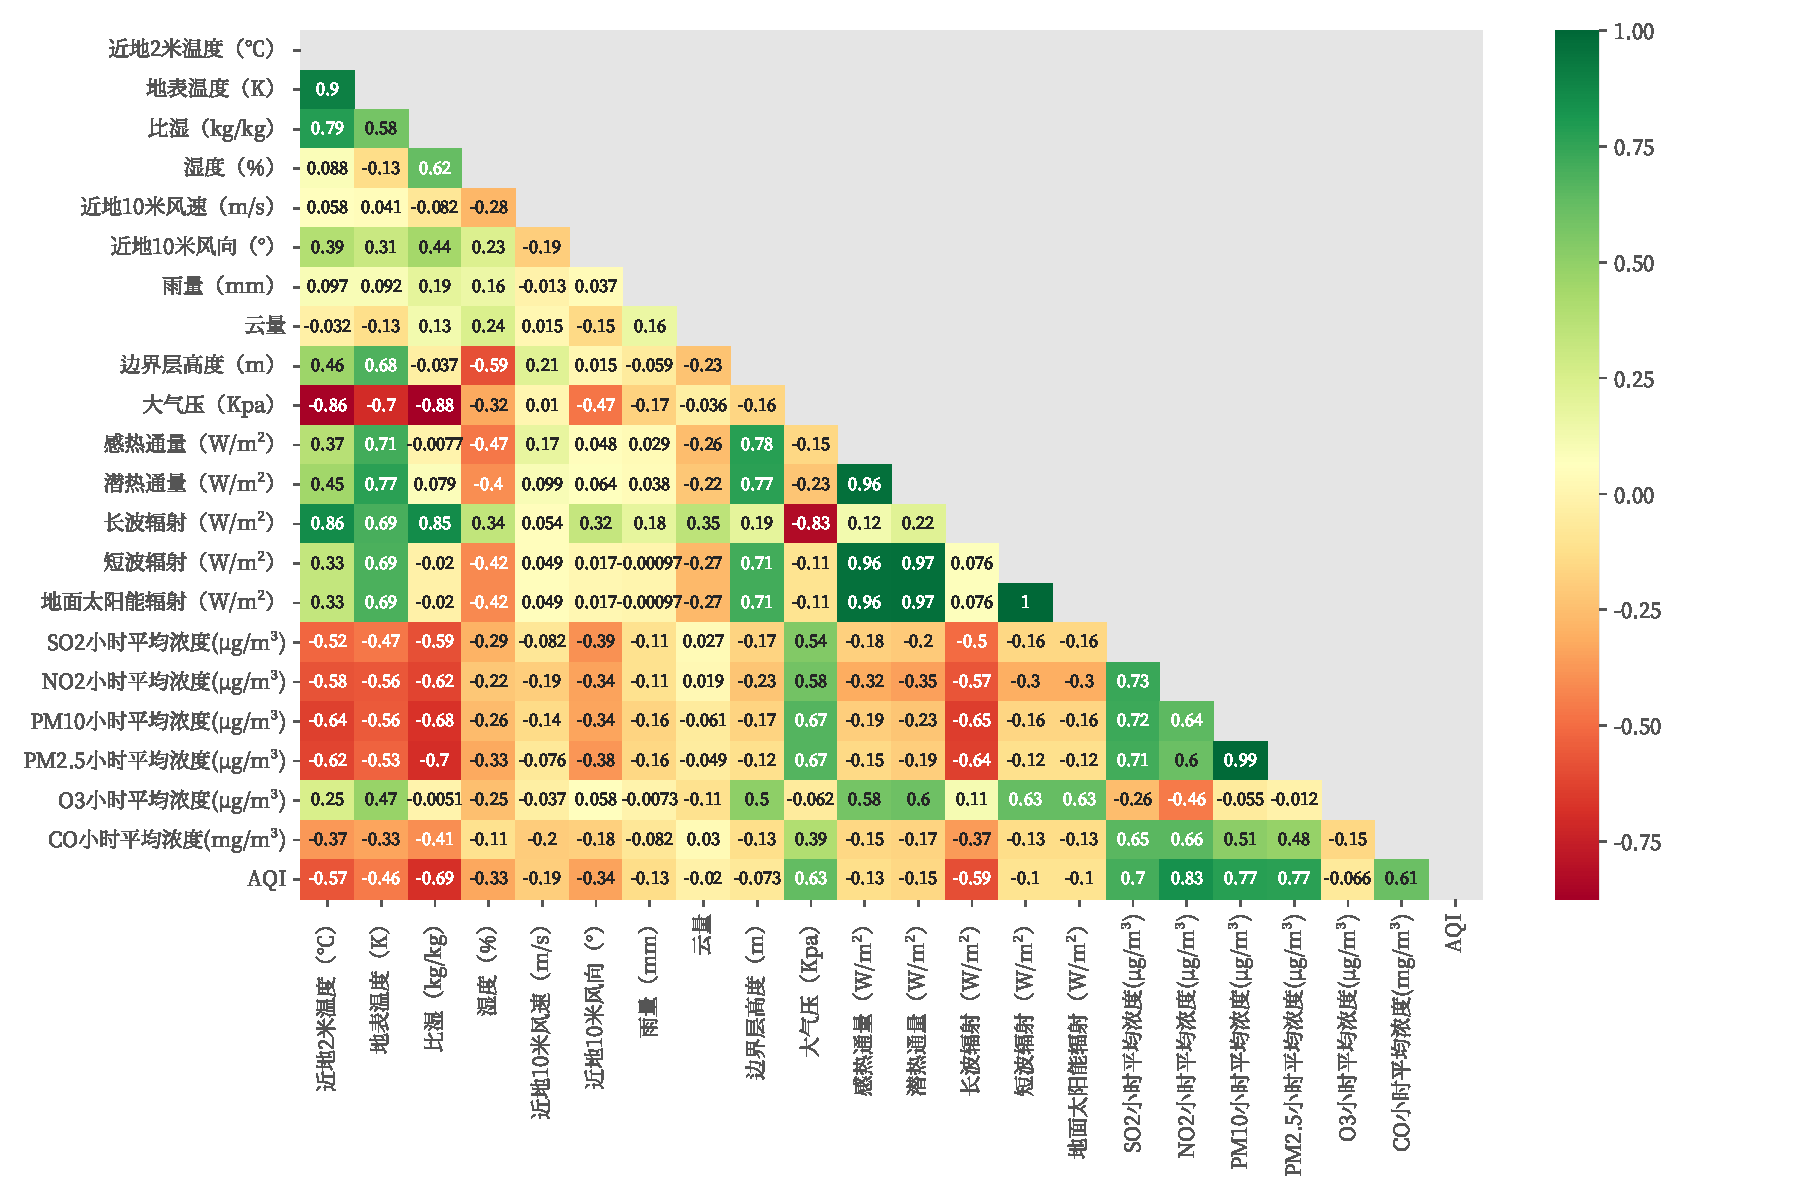
\includegraphics[width=5in]{A1-0相关性分析.pdf}
    \end{minipage}}

    \subfigure[pic5.]{
    \begin{minipage}[t]{0.25\linewidth}
    \centering
    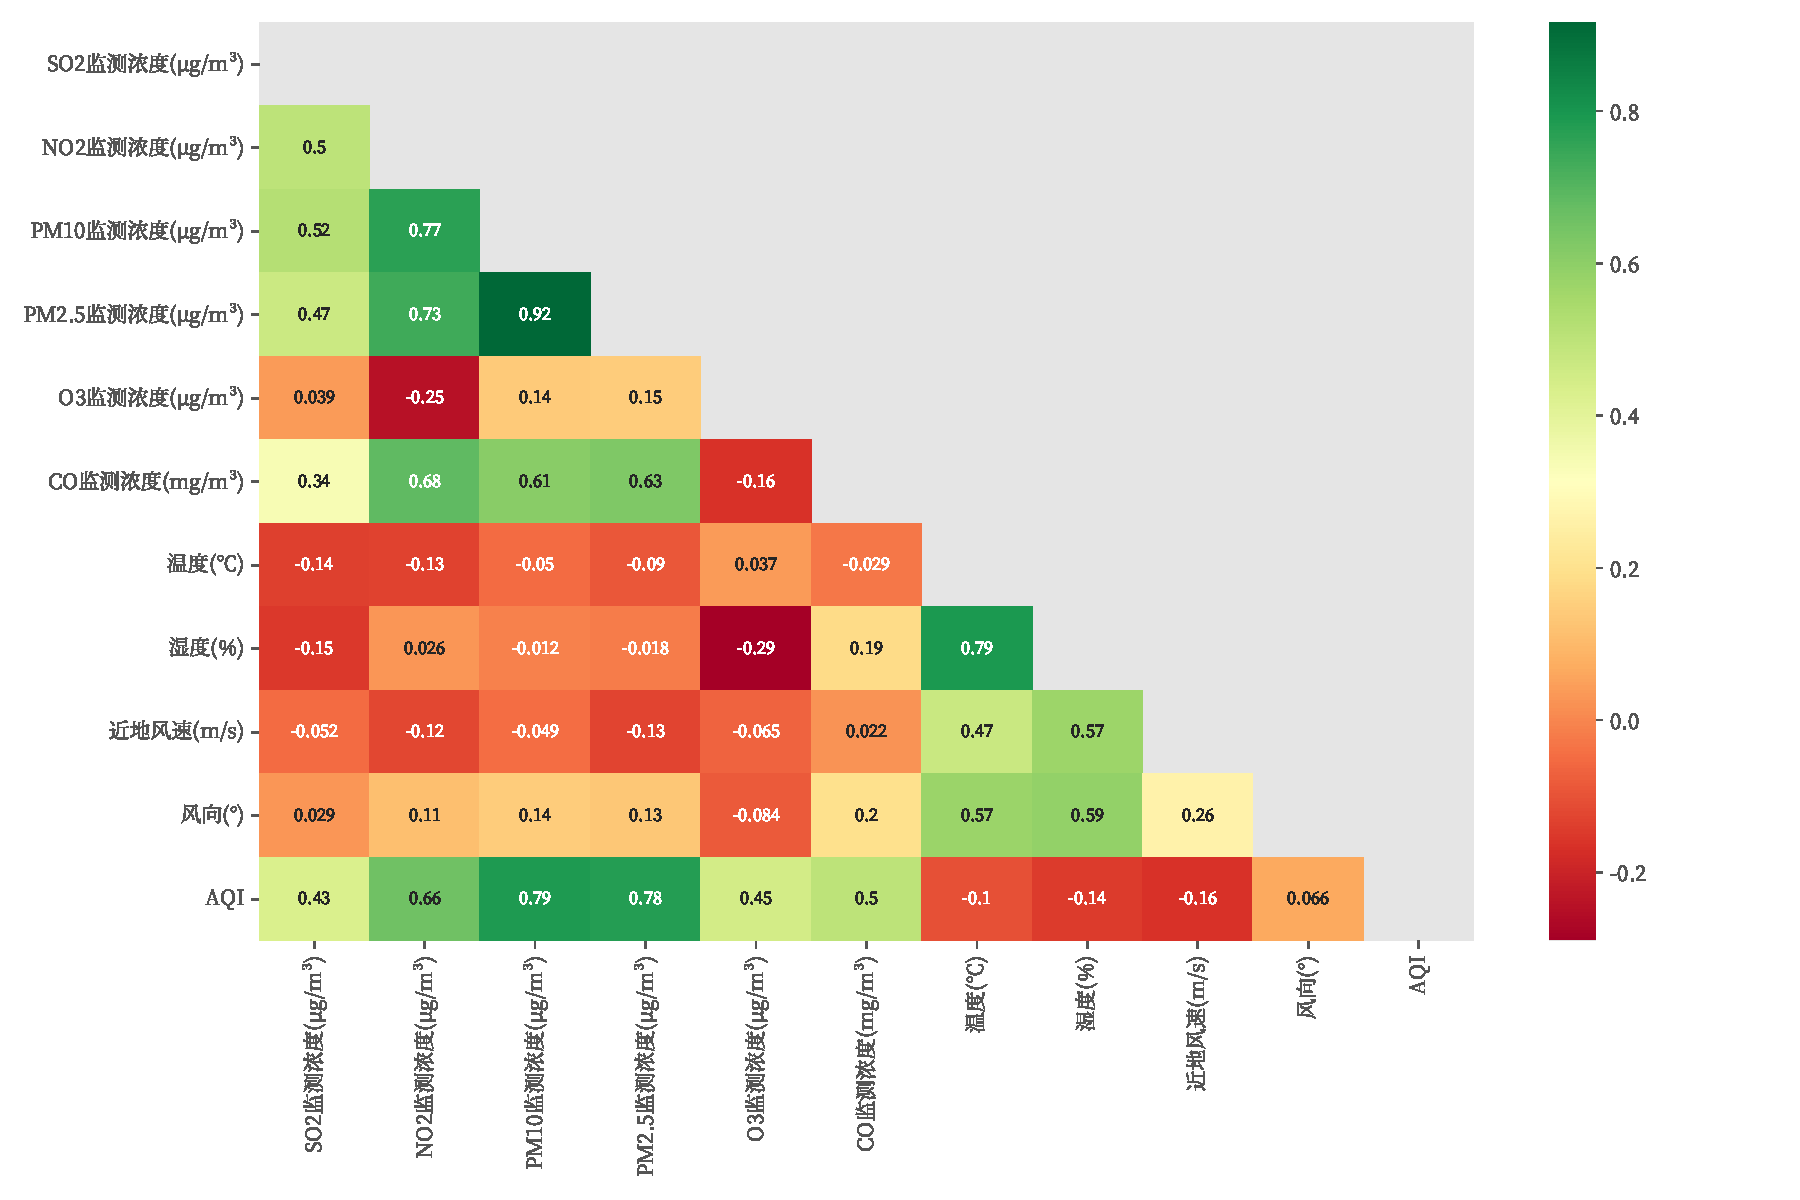
\includegraphics[width=5in]{A1-1相关性分析.pdf}
    \end{minipage}}

    \subfigure[pic6.]{
    \begin{minipage}[t]{0.25\linewidth}
    \centering
    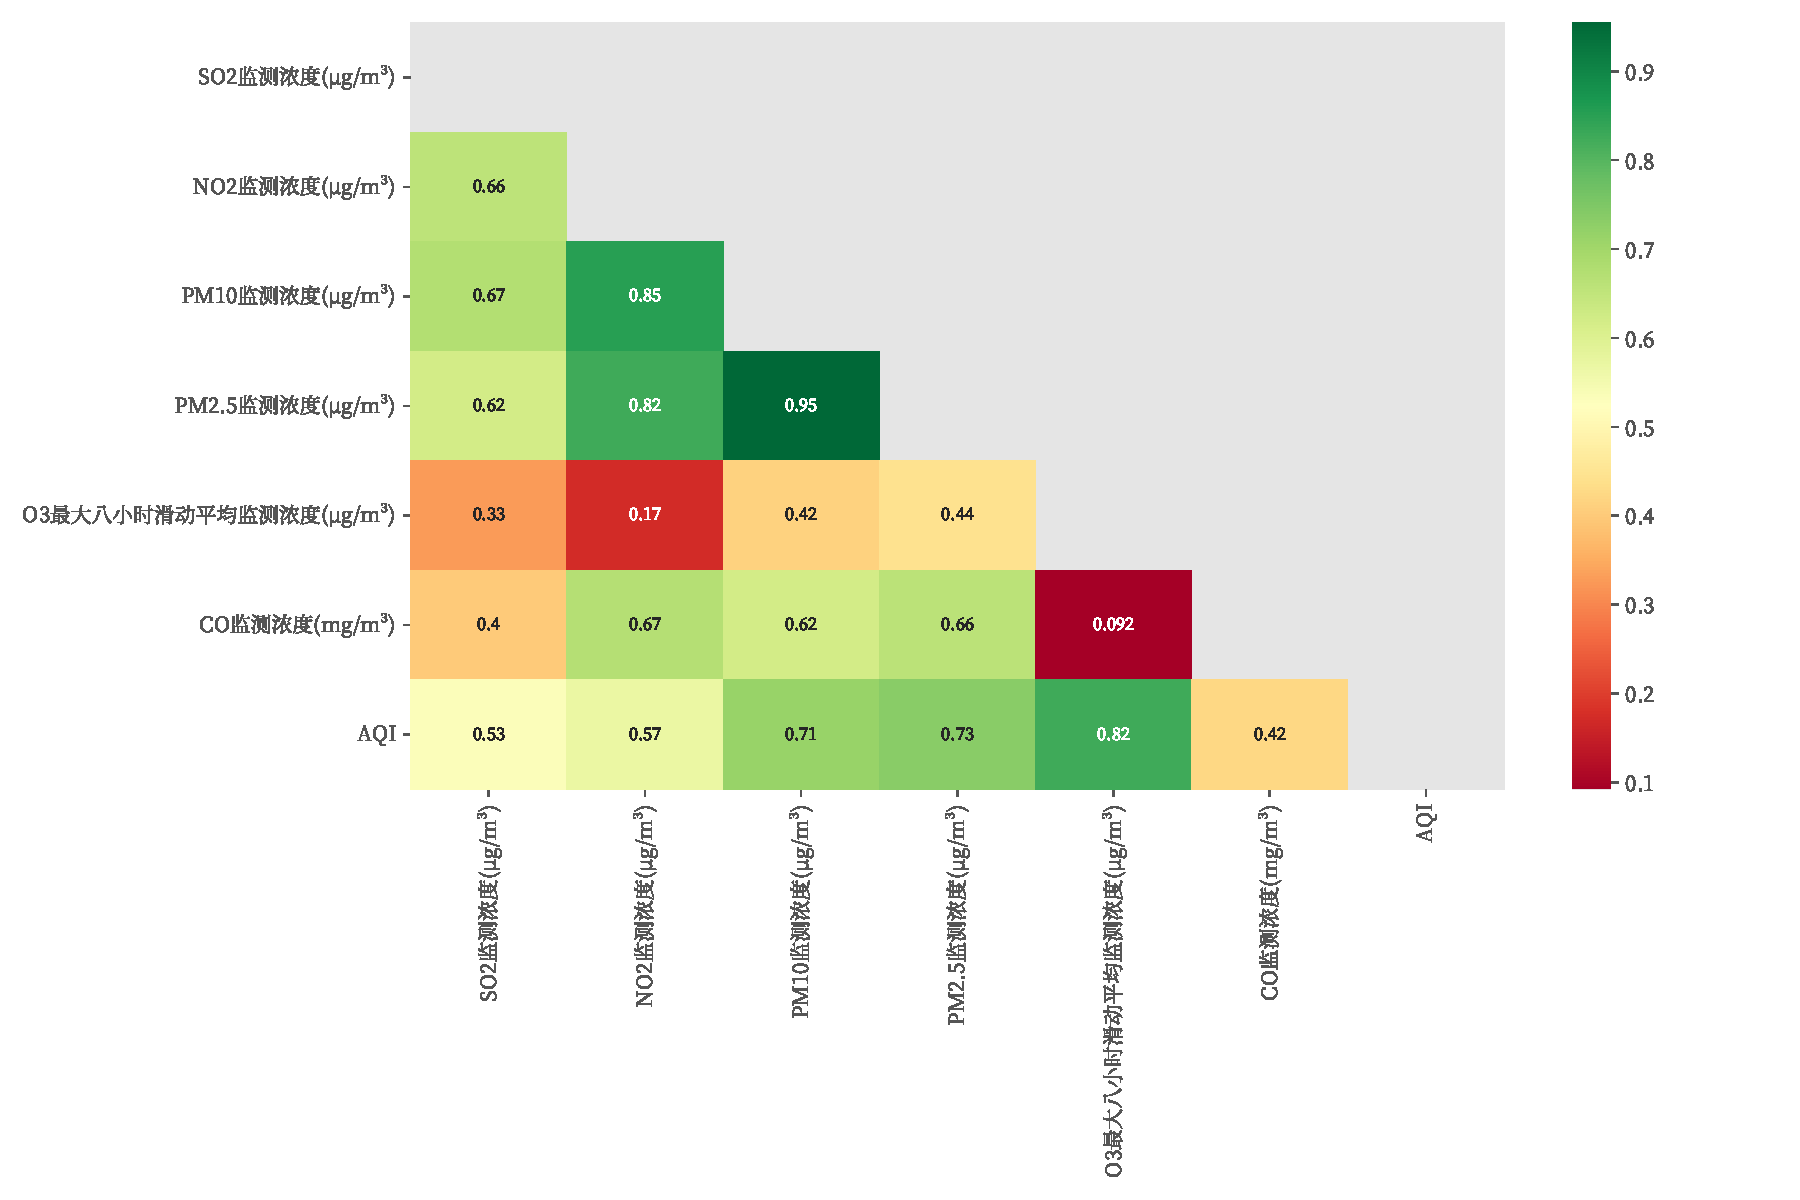
\includegraphics[width=5in]{A1-2相关性分析.pdf}
    \end{minipage}}

    \subfigure[pic7.]{
    \begin{minipage}[t]{0.25\linewidth}
    \centering
    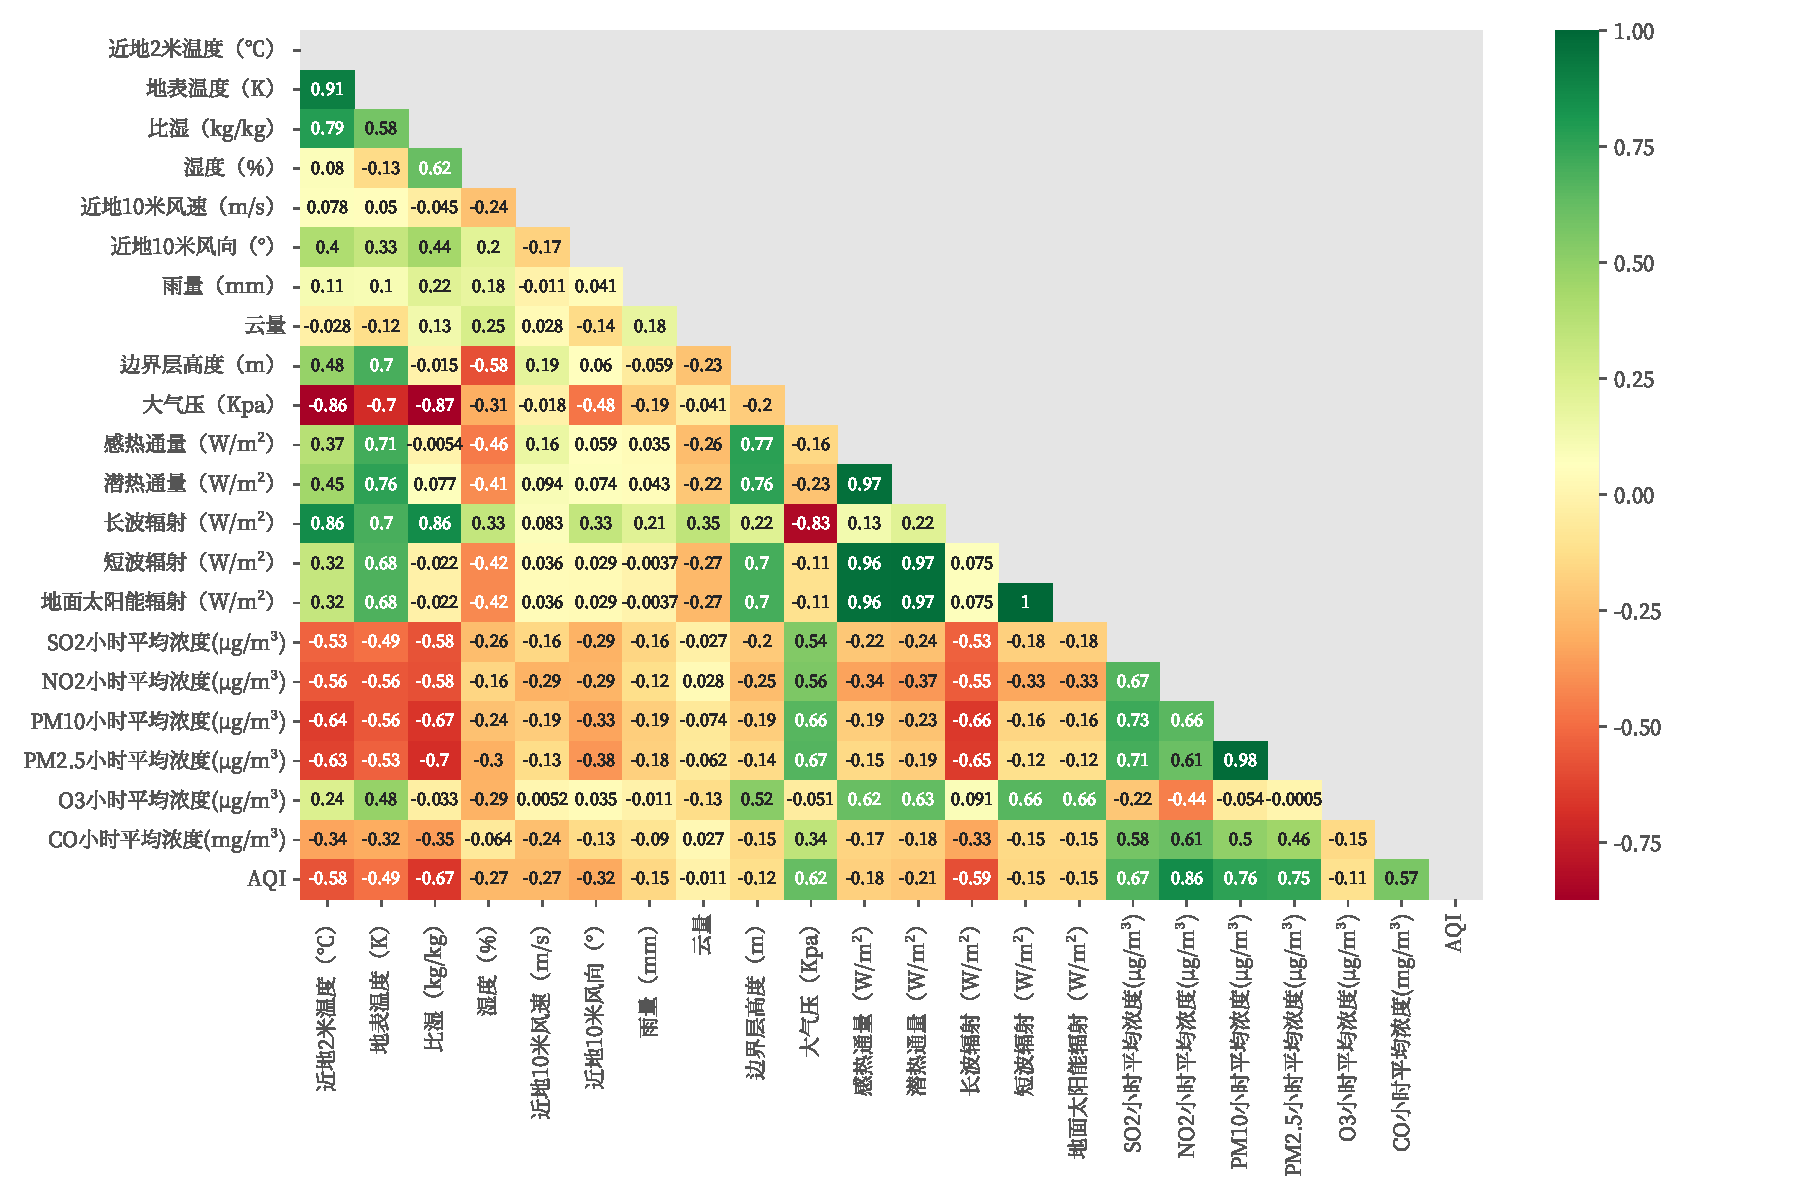
\includegraphics[width=5in]{A2-0相关性分析.pdf}
    \end{minipage}}

    \subfigure[pic8.]{
    \begin{minipage}[t]{0.25\linewidth}
    \centering
    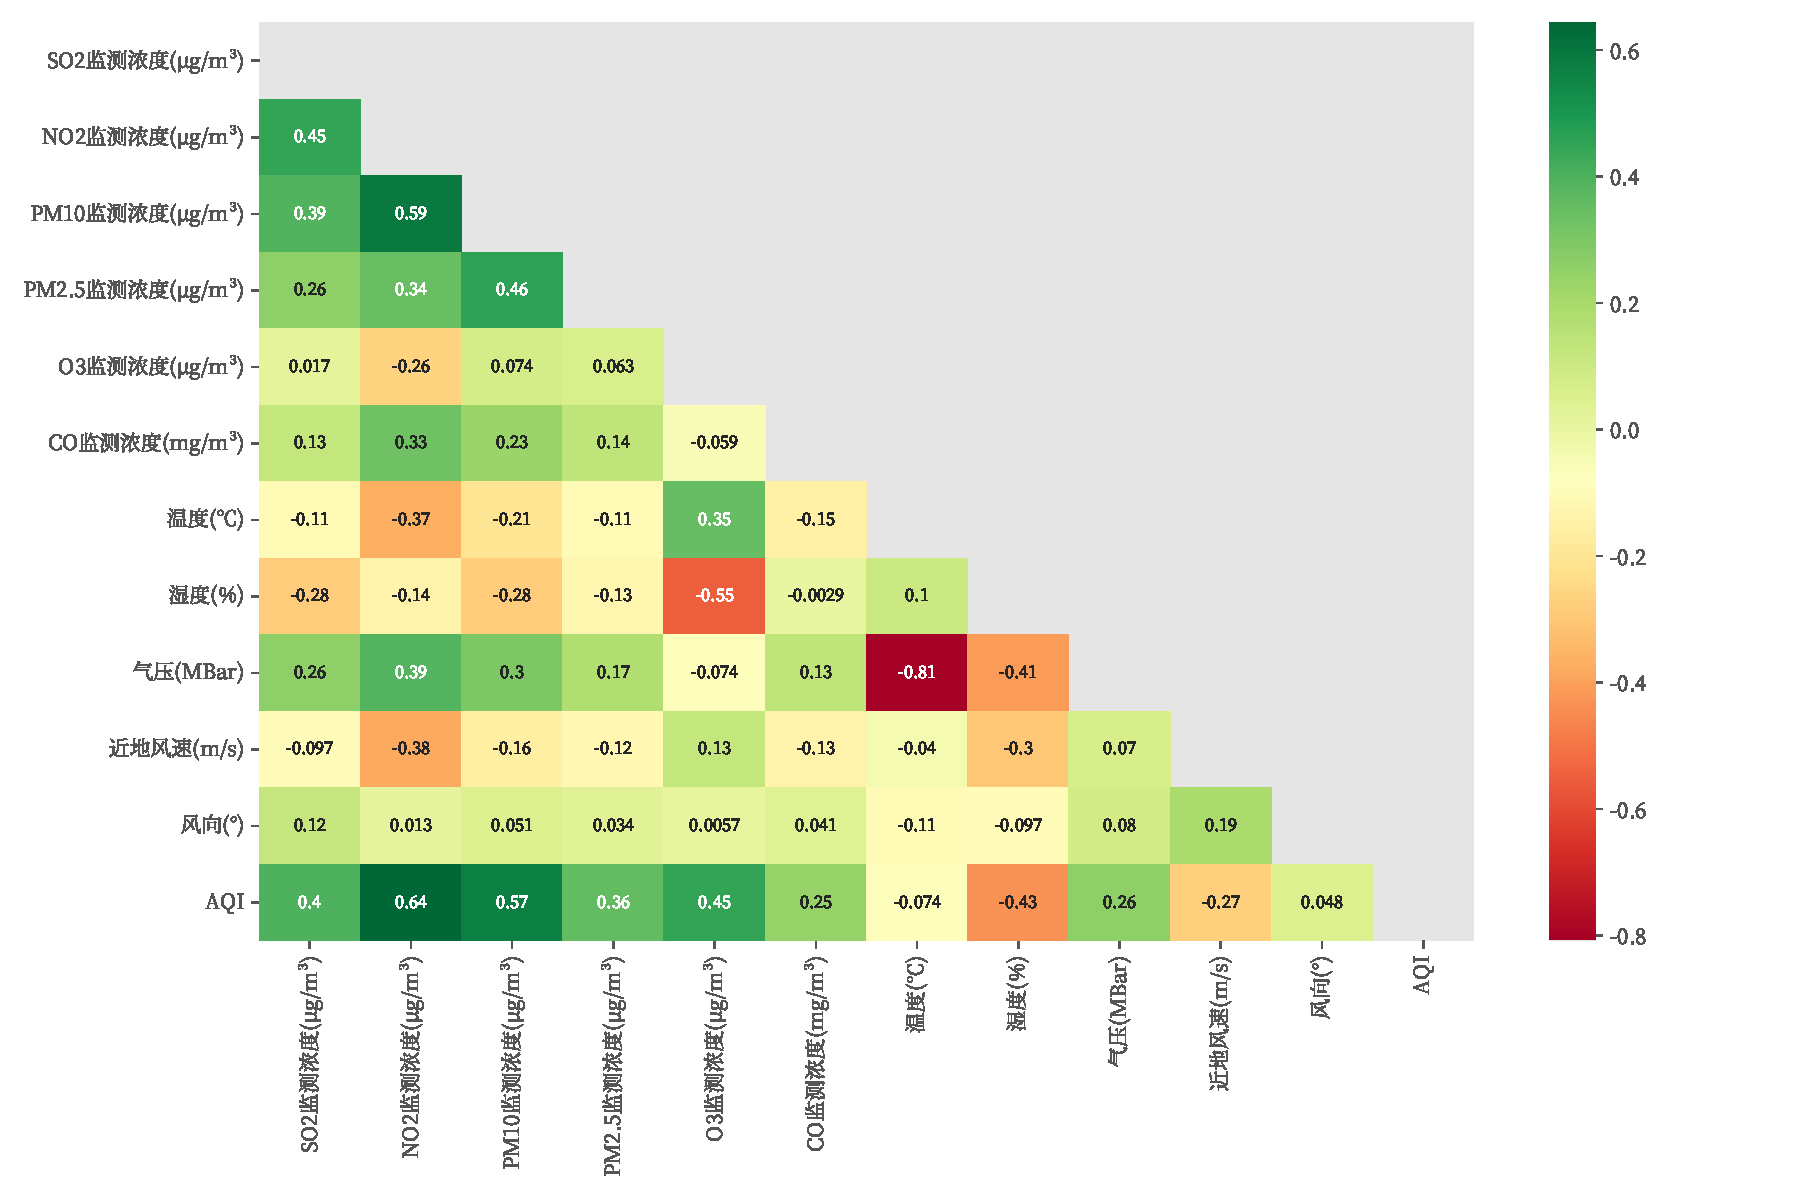
\includegraphics[width=5in]{A2-1相关性分析.pdf}
    \end{minipage}}

    \subfigure[pic9.]{
    \begin{minipage}[t]{0.25\linewidth}
    \centering
    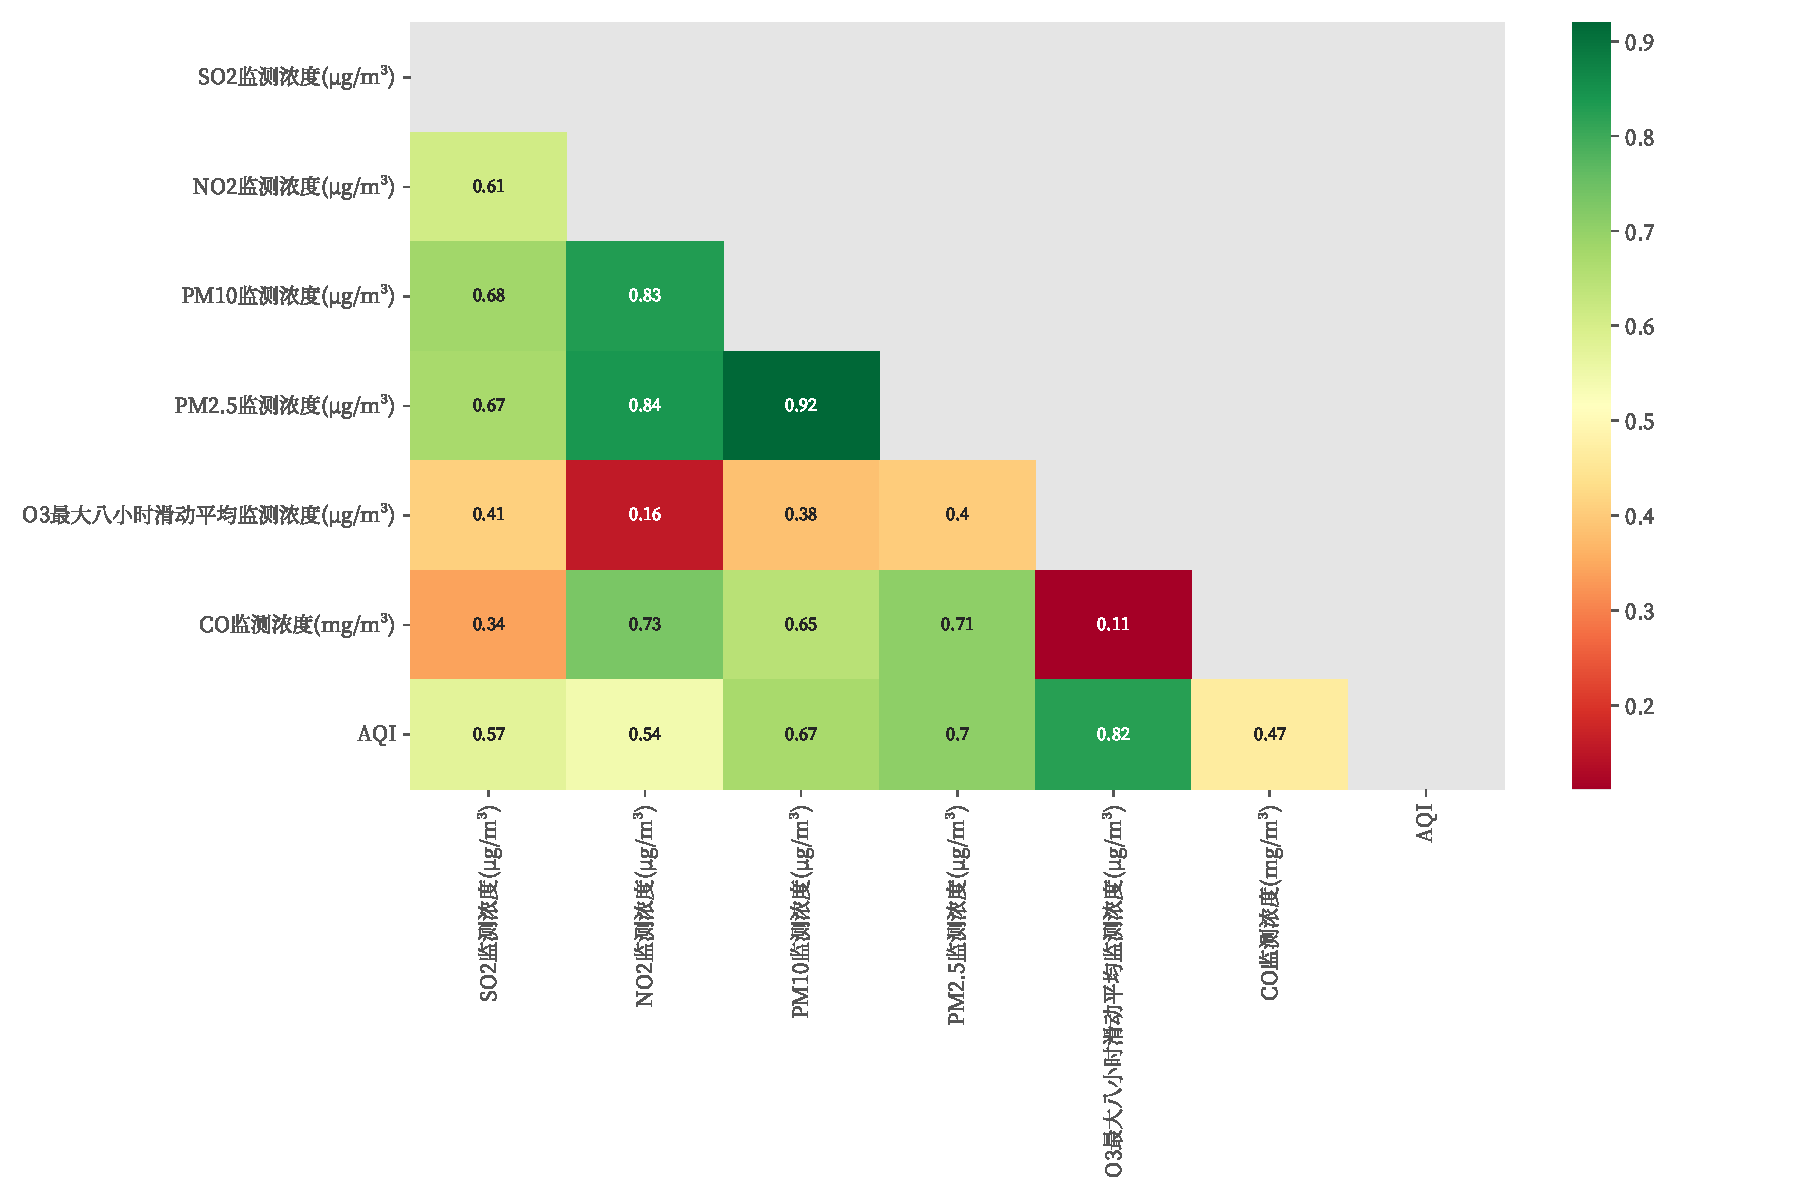
\includegraphics[width=5in]{A2-2相关性分析.pdf}
    \end{minipage}}

    \subfigure[pic10.]{
    \begin{minipage}[t]{0.25\linewidth}
    \centering
    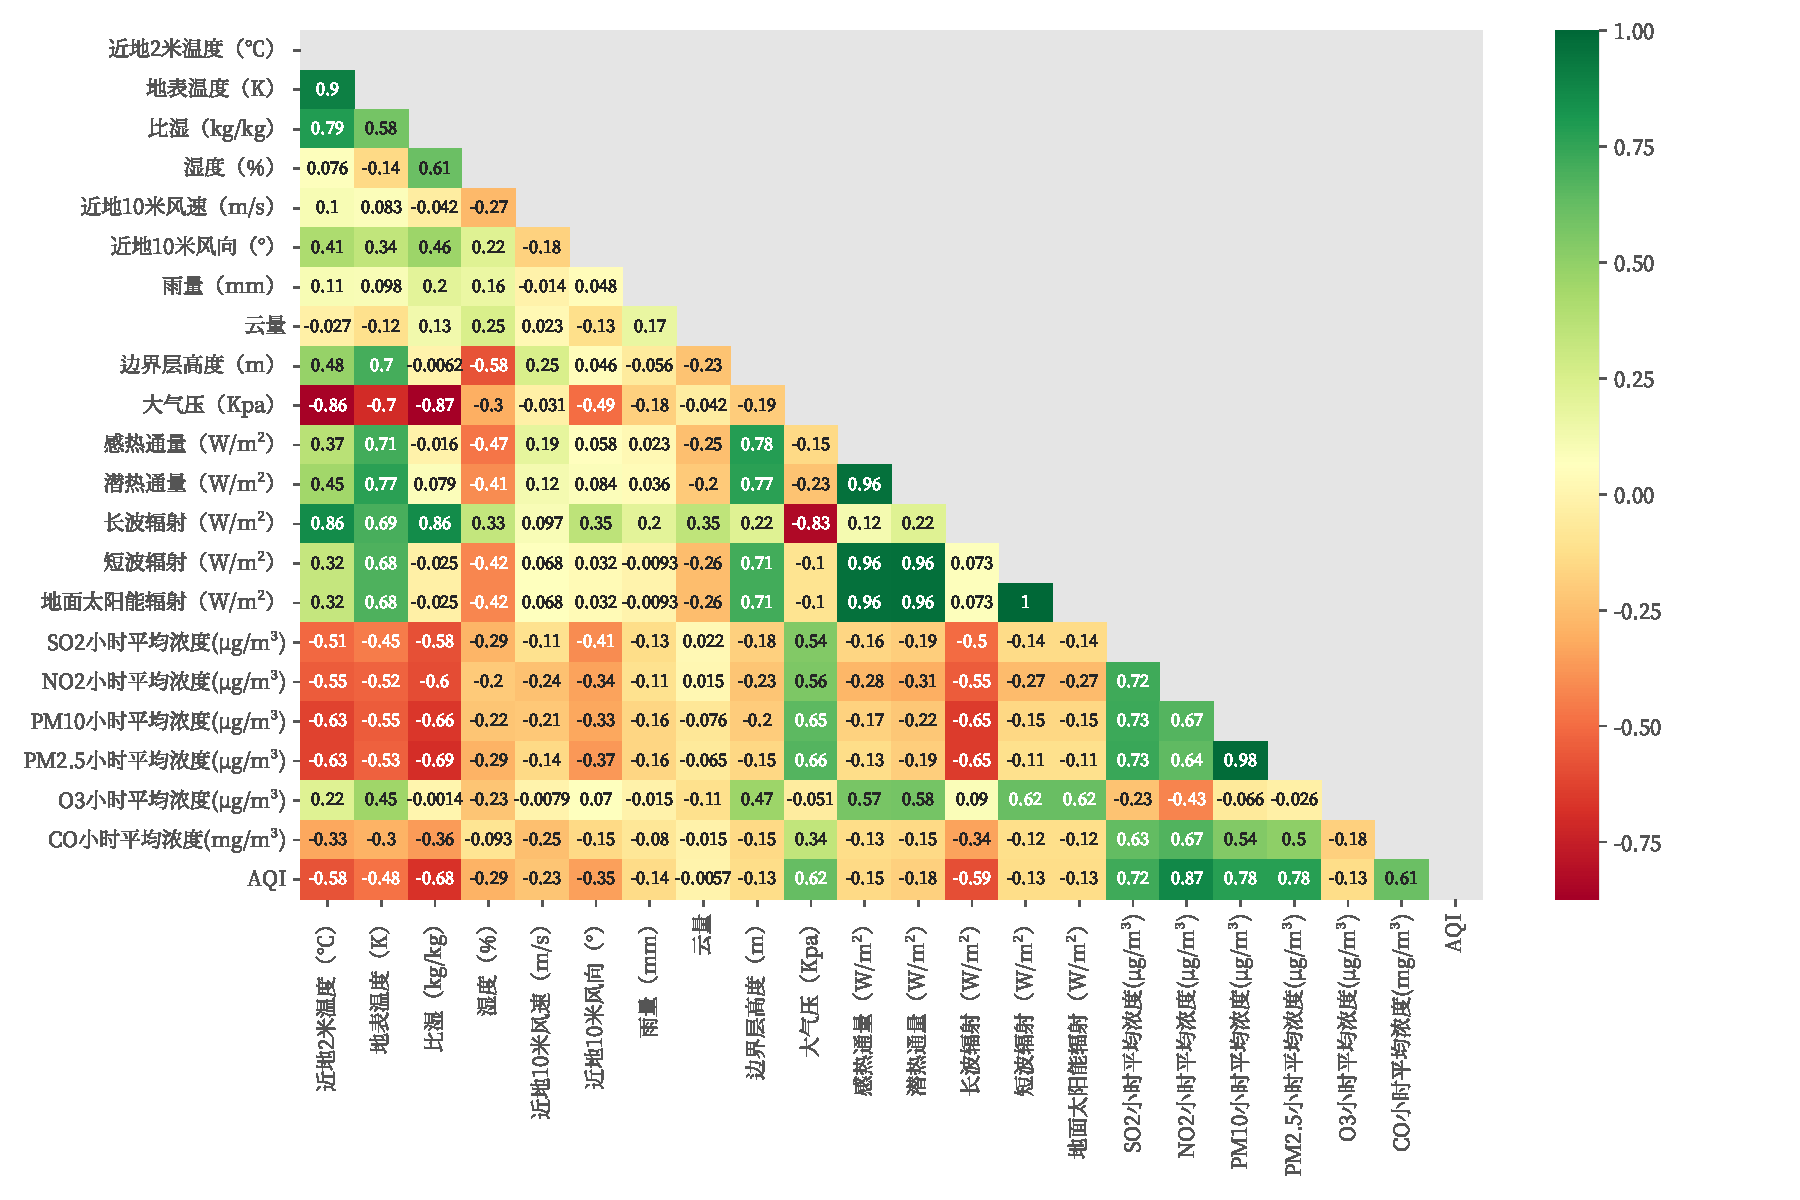
\includegraphics[width=5in]{A3-0相关性分析.pdf}
    \end{minipage}}

    \subfigure[pic11.]{
    \begin{minipage}[t]{0.25\linewidth}
    \centering
    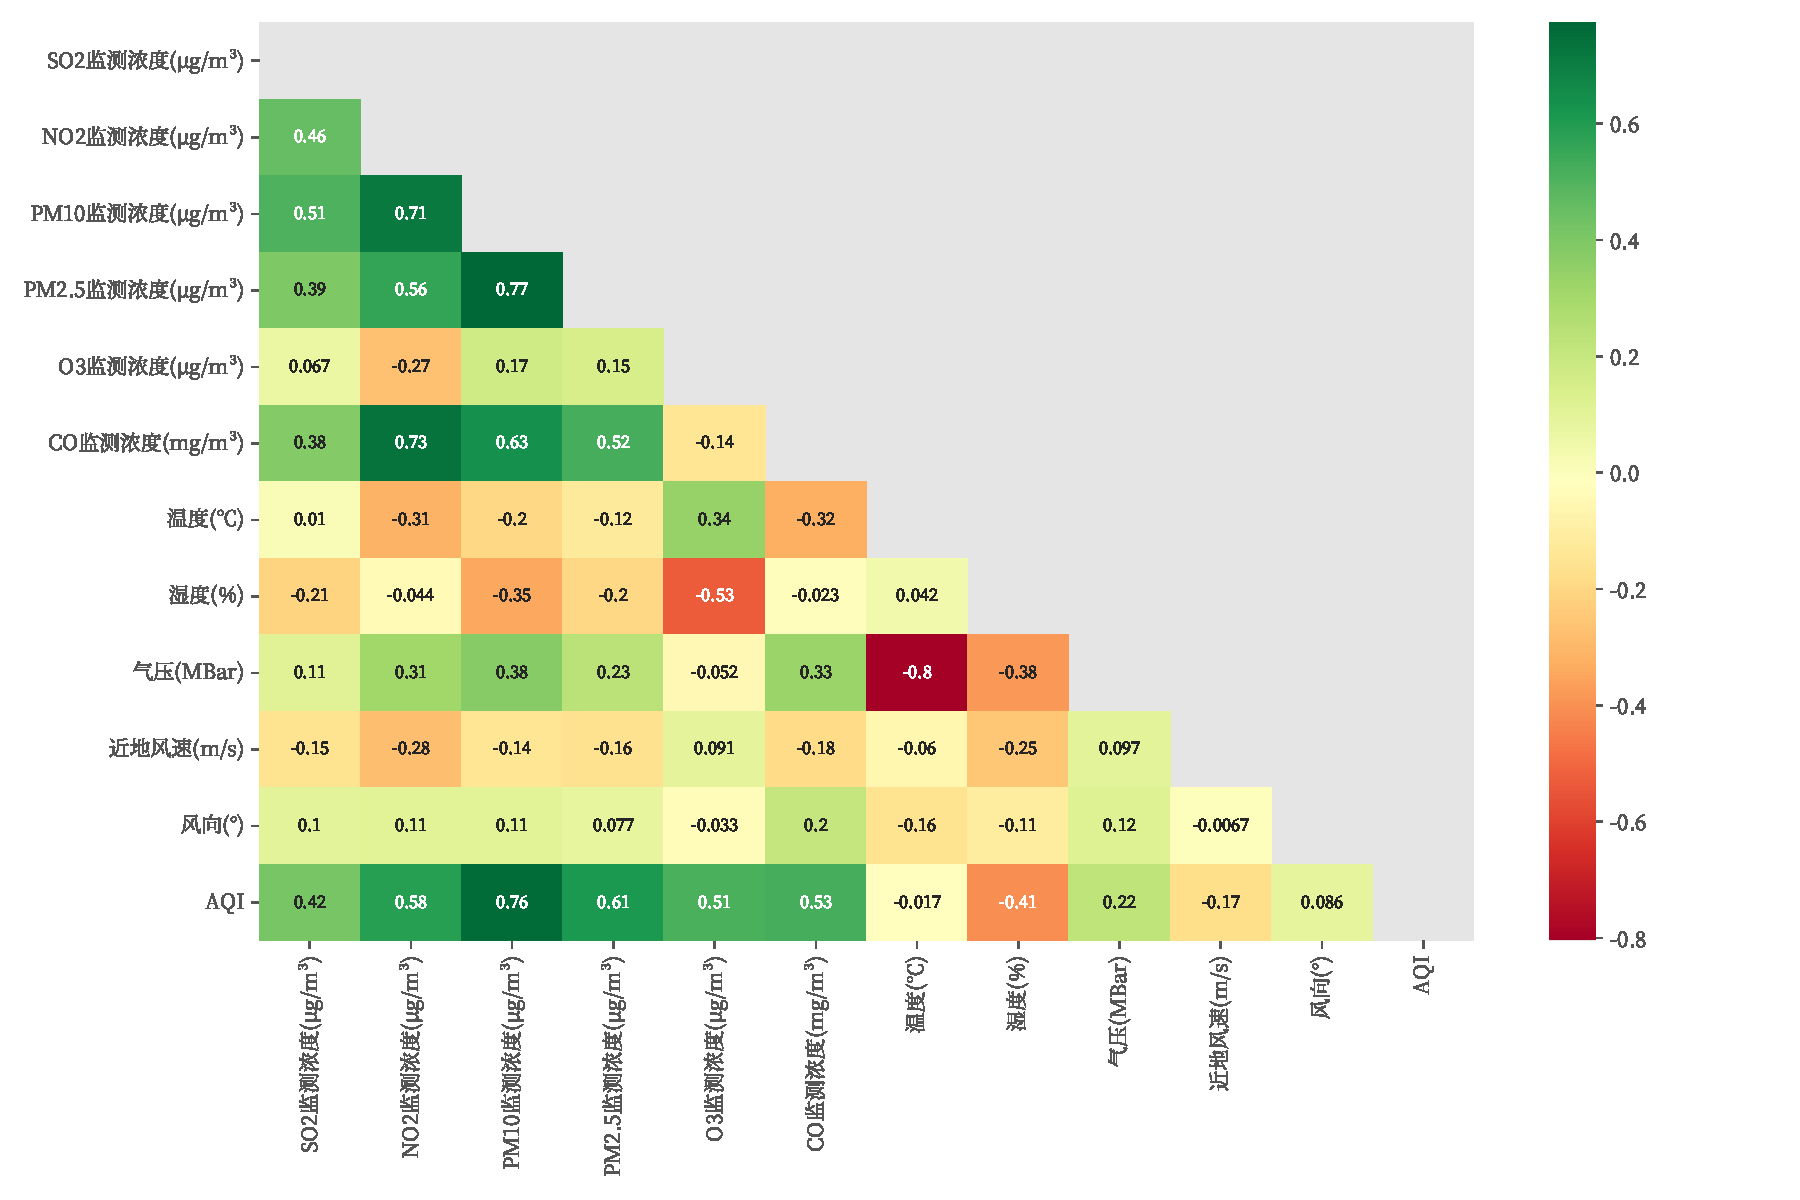
\includegraphics[width=5in]{A3-1相关性分析.pdf}
    \end{minipage}}

    \subfigure[pic12.]{
    \begin{minipage}[t]{0.25\linewidth}
    \centering
    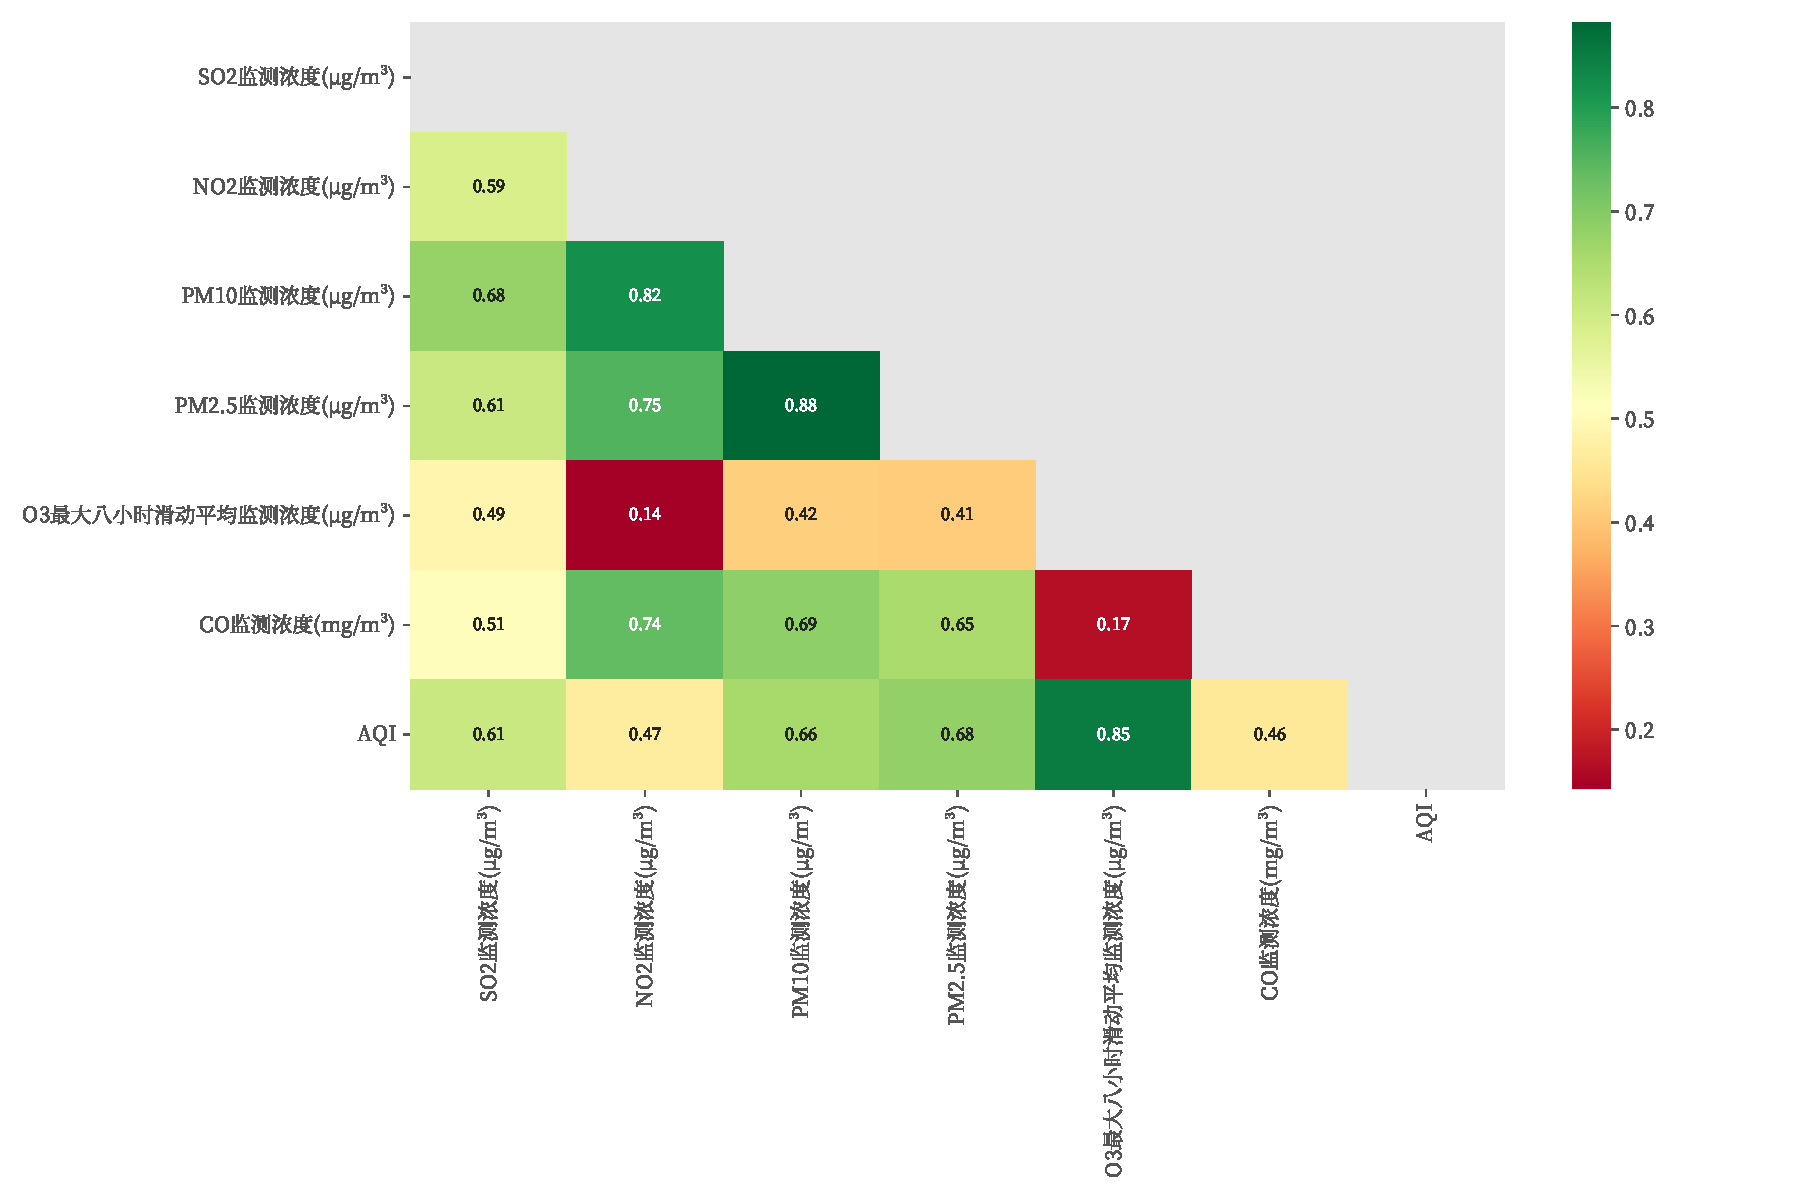
\includegraphics[width=5in]{A3-2相关性分析.pdf}
    \end{minipage}}

    \subfigure[pic13.]{
    \begin{minipage}[t]{0.25\linewidth}
    \centering
    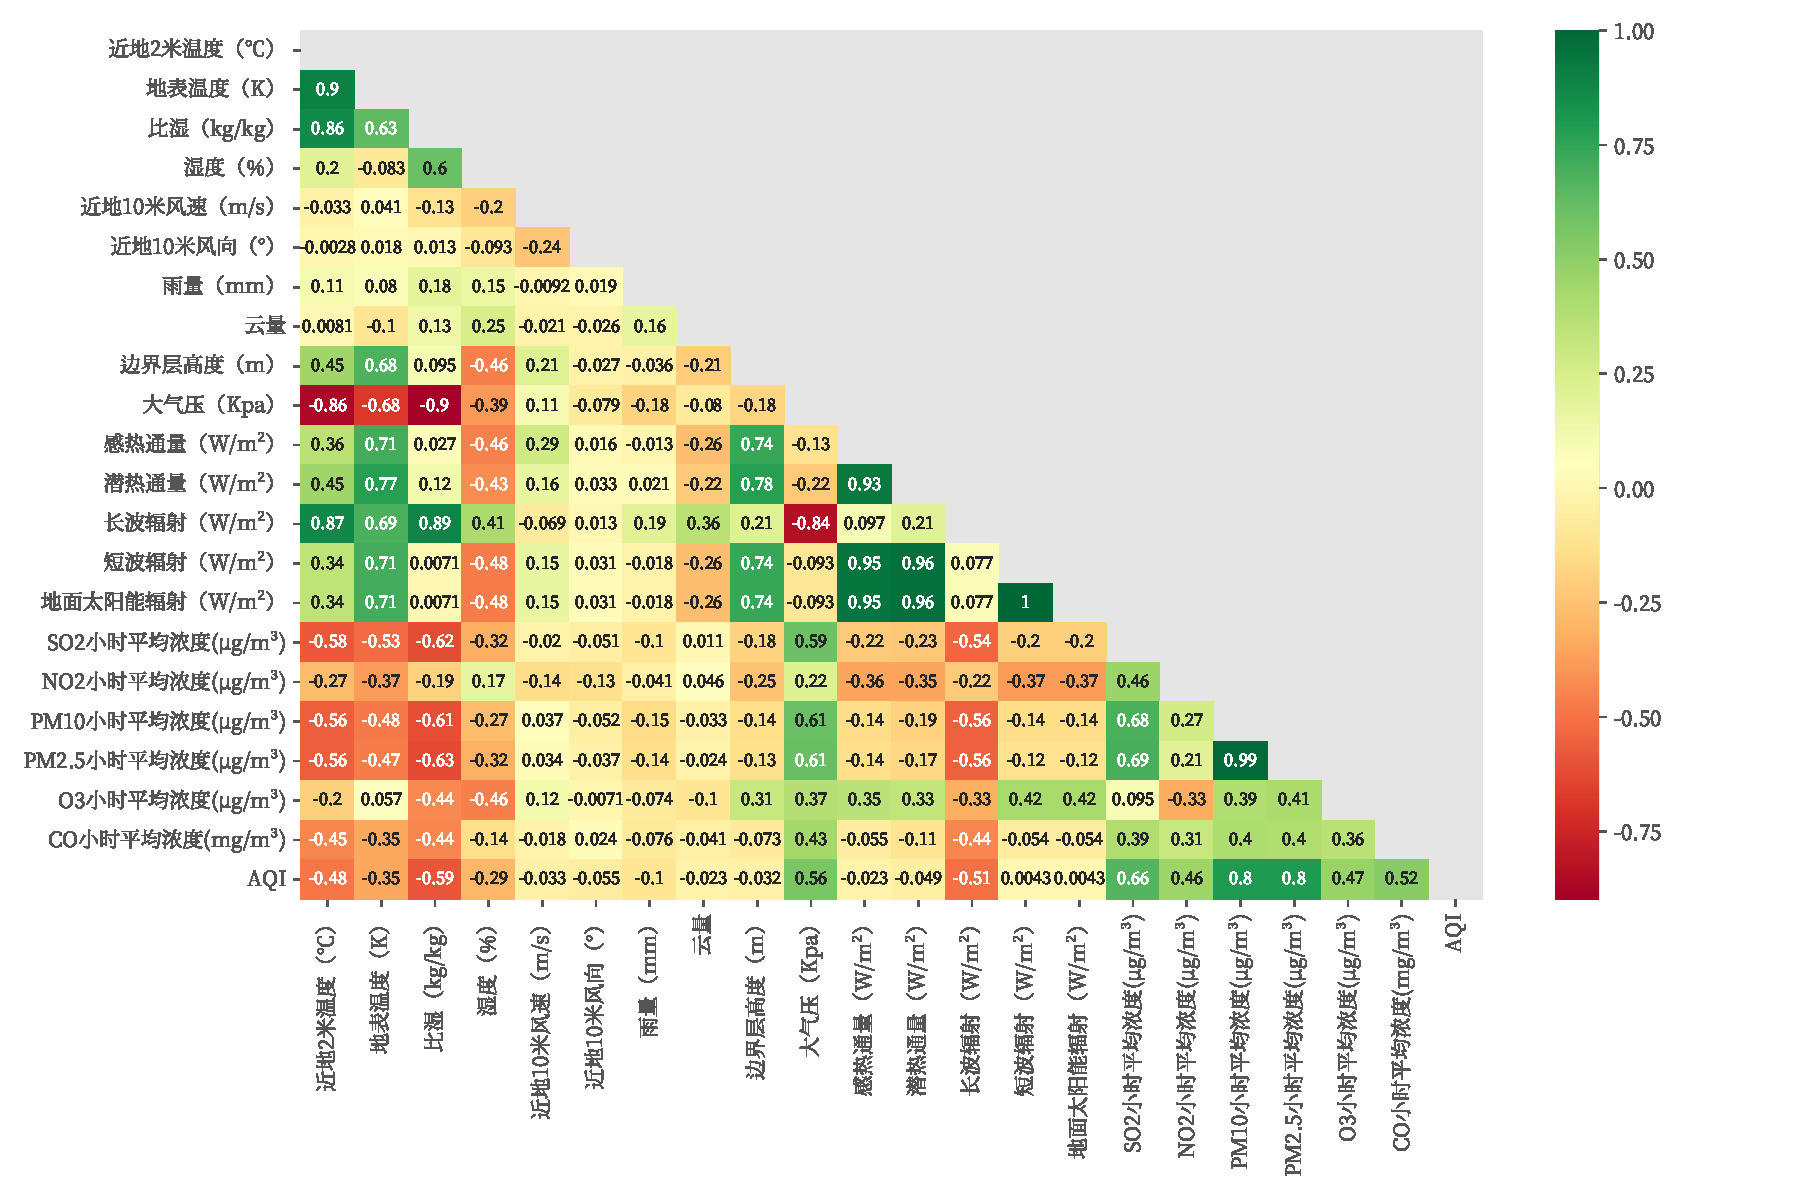
\includegraphics[width=5in]{B-0相关性分析.pdf}
    \end{minipage}}

    \subfigure[pic14.]{
    \begin{minipage}[t]{0.25\linewidth}
    \centering
    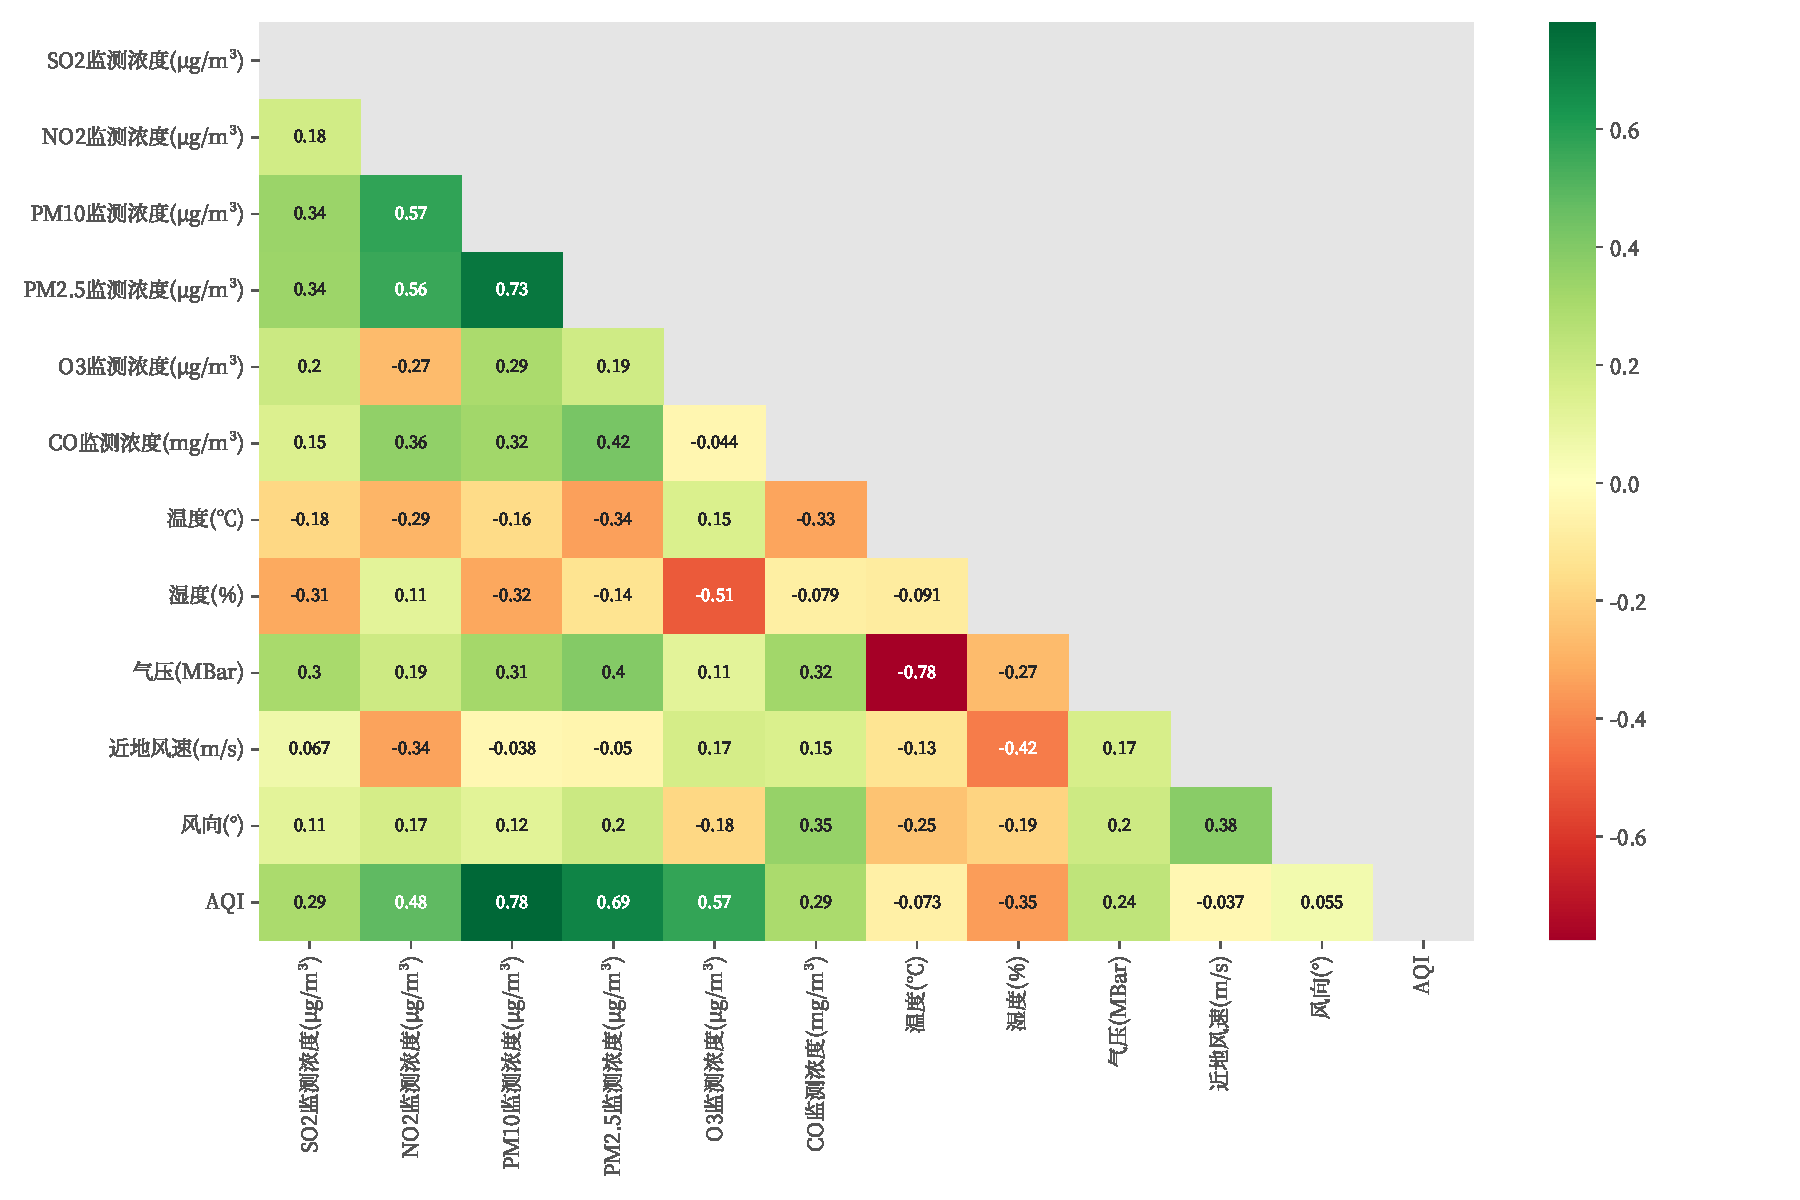
\includegraphics[width=5in]{B-1相关性分析.pdf}
    \end{minipage}}

    \subfigure[pic15.]{
    \begin{minipage}[t]{0.25\linewidth}
    \centering
    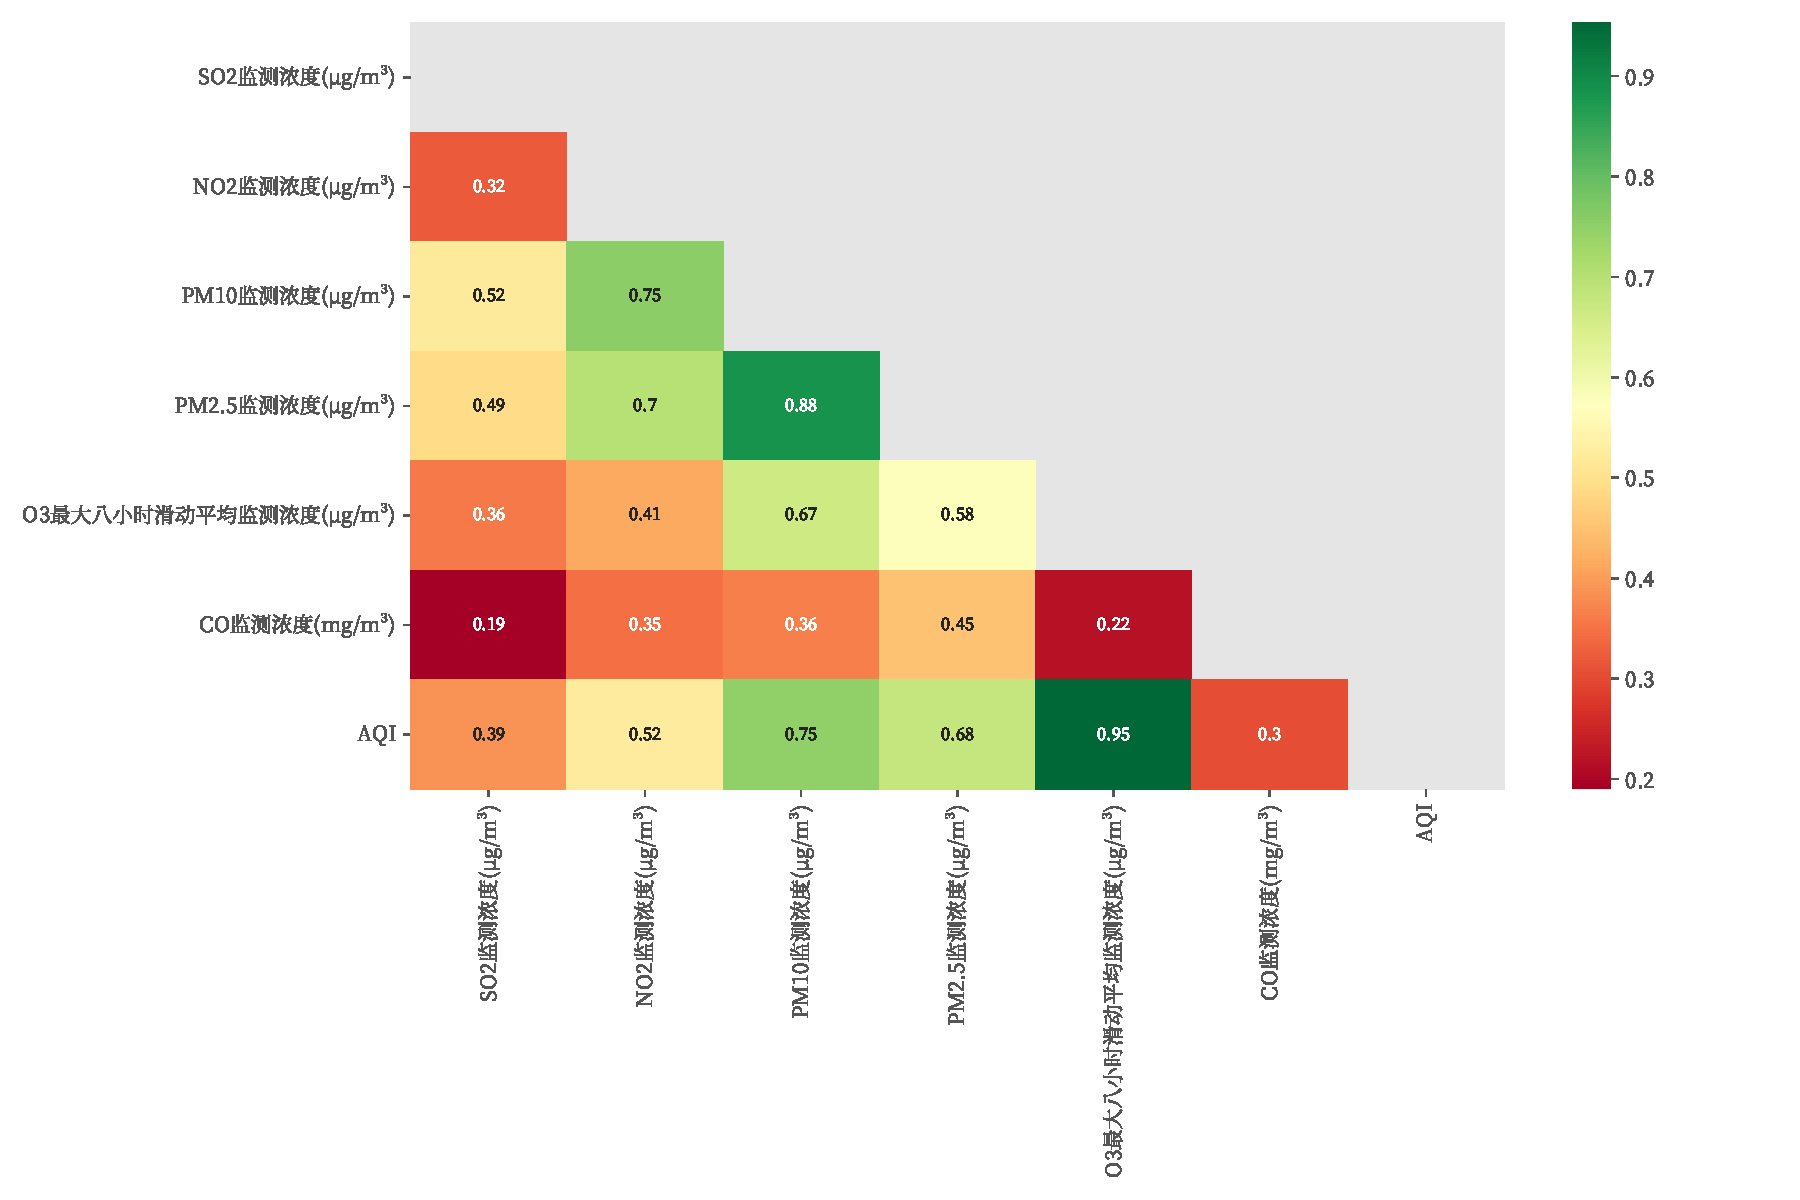
\includegraphics[width=5in]{B-2相关性分析.pdf}
    \end{minipage}}

    \subfigure[pic16.]{
    \begin{minipage}[t]{0.25\linewidth}
    \centering
    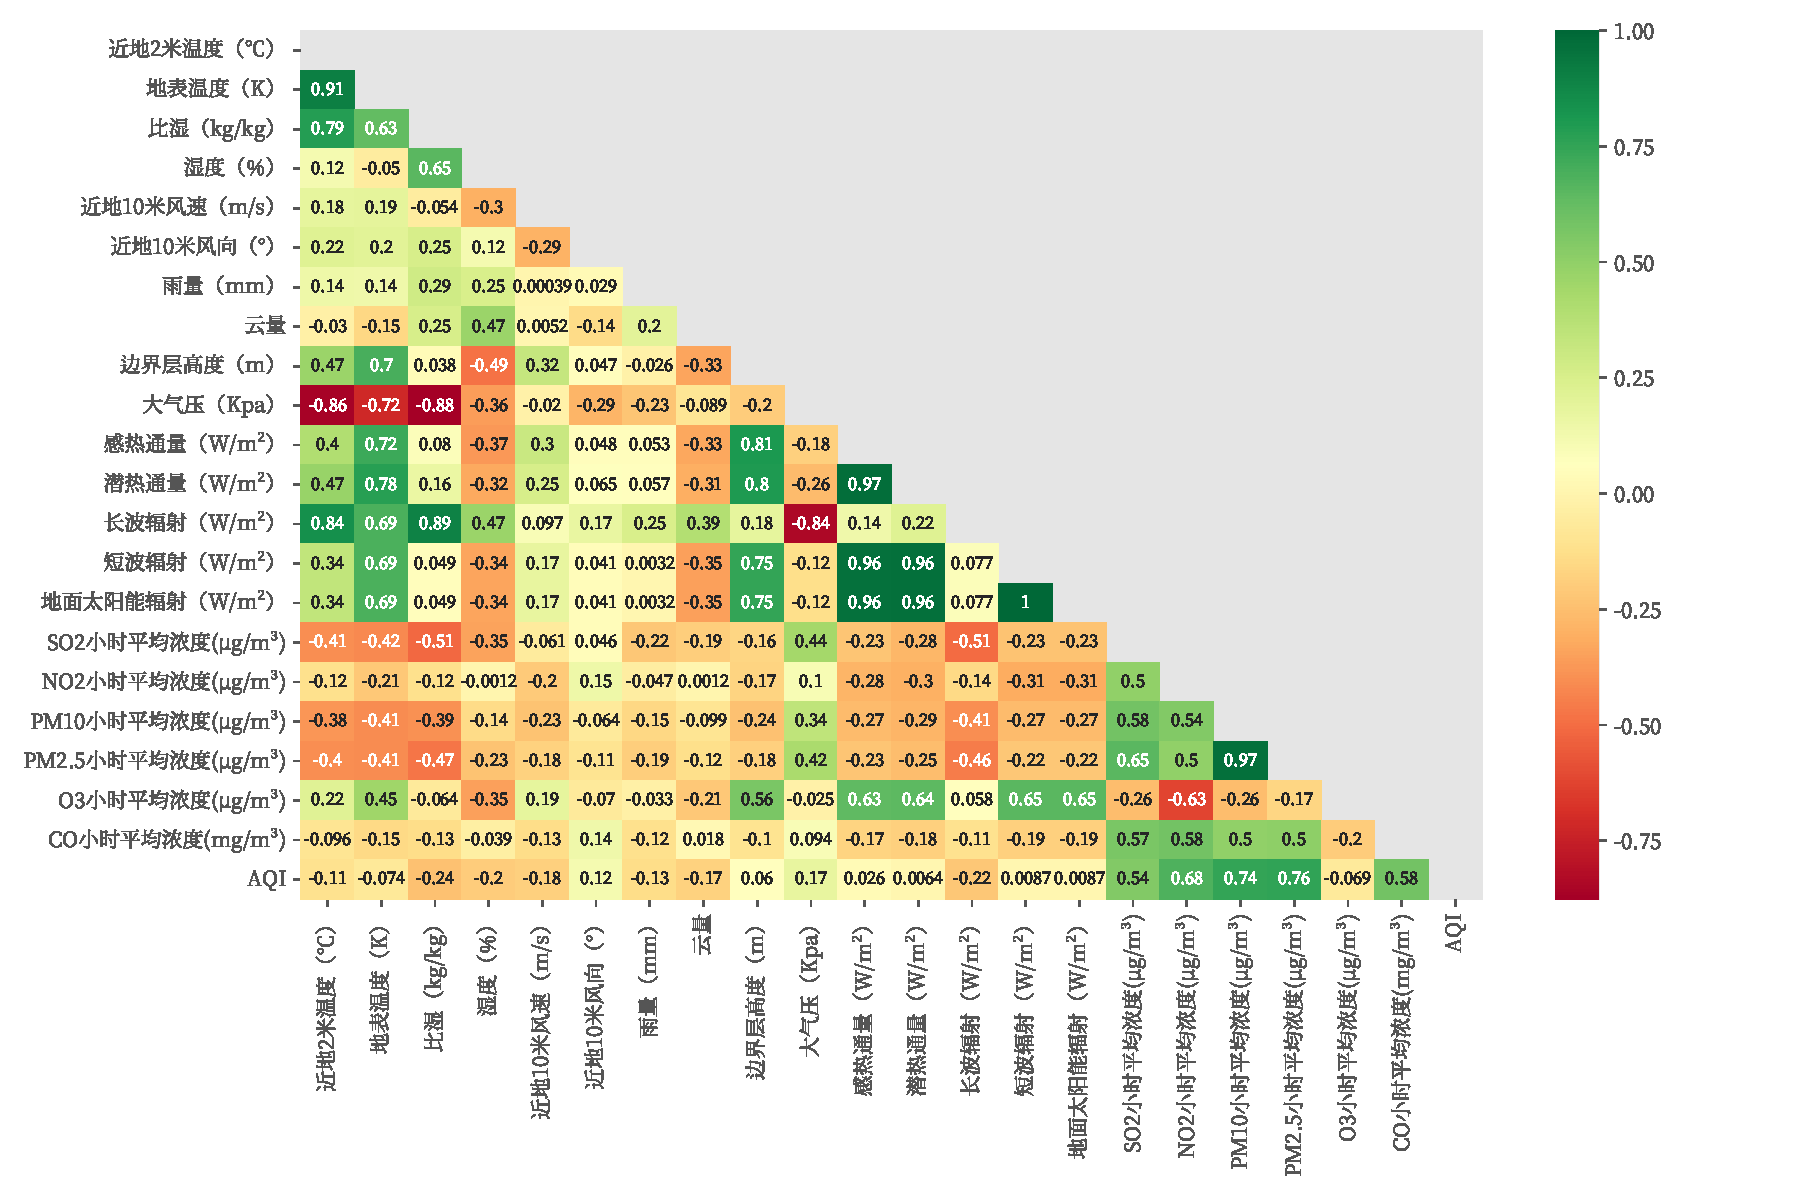
\includegraphics[width=5in]{C-0相关性分析.pdf}
    \end{minipage}}

    \subfigure[pic17.]{
    \begin{minipage}[t]{0.25\linewidth}
    \centering
    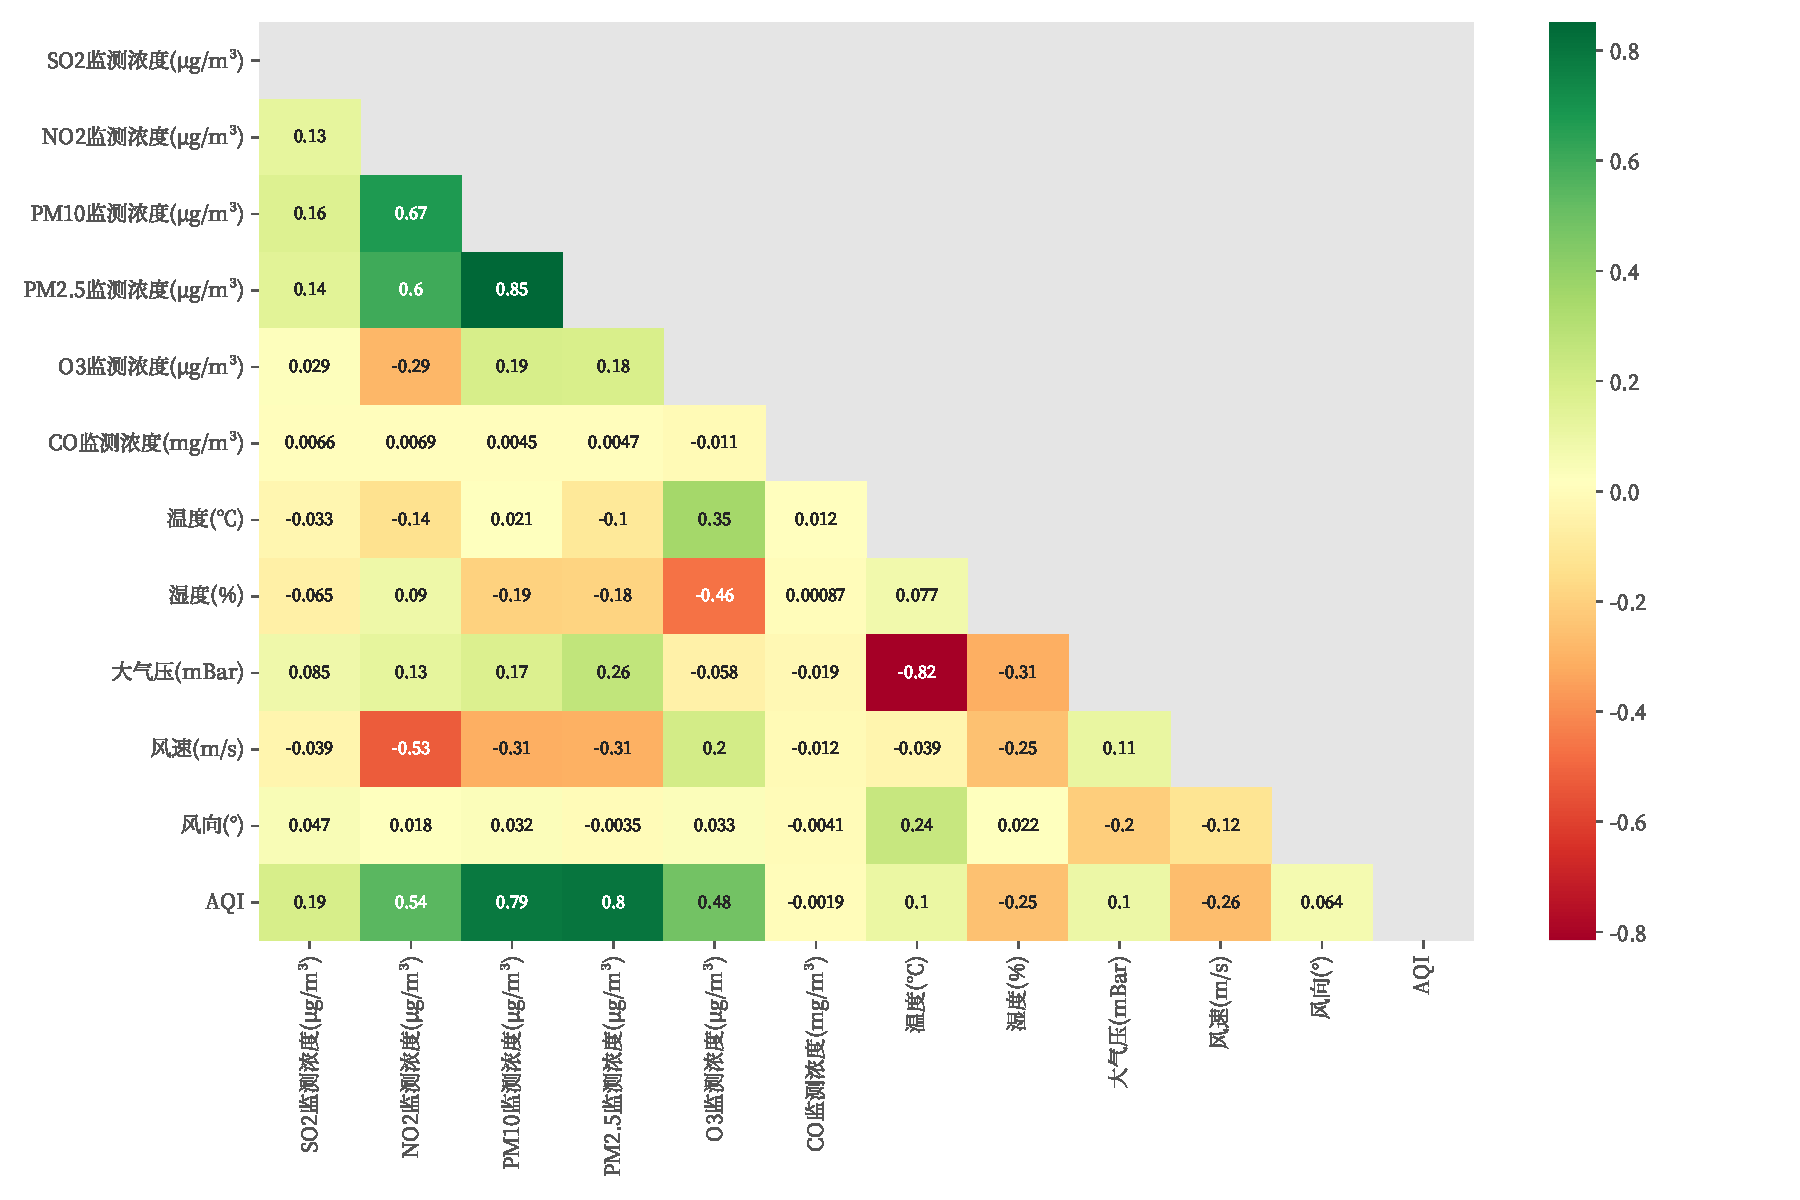
\includegraphics[width=5in]{C-1相关性分析.pdf}
    \end{minipage}}

    \subfigure[pic18.]{
    \begin{minipage}[t]{0.25\linewidth}
    \centering
    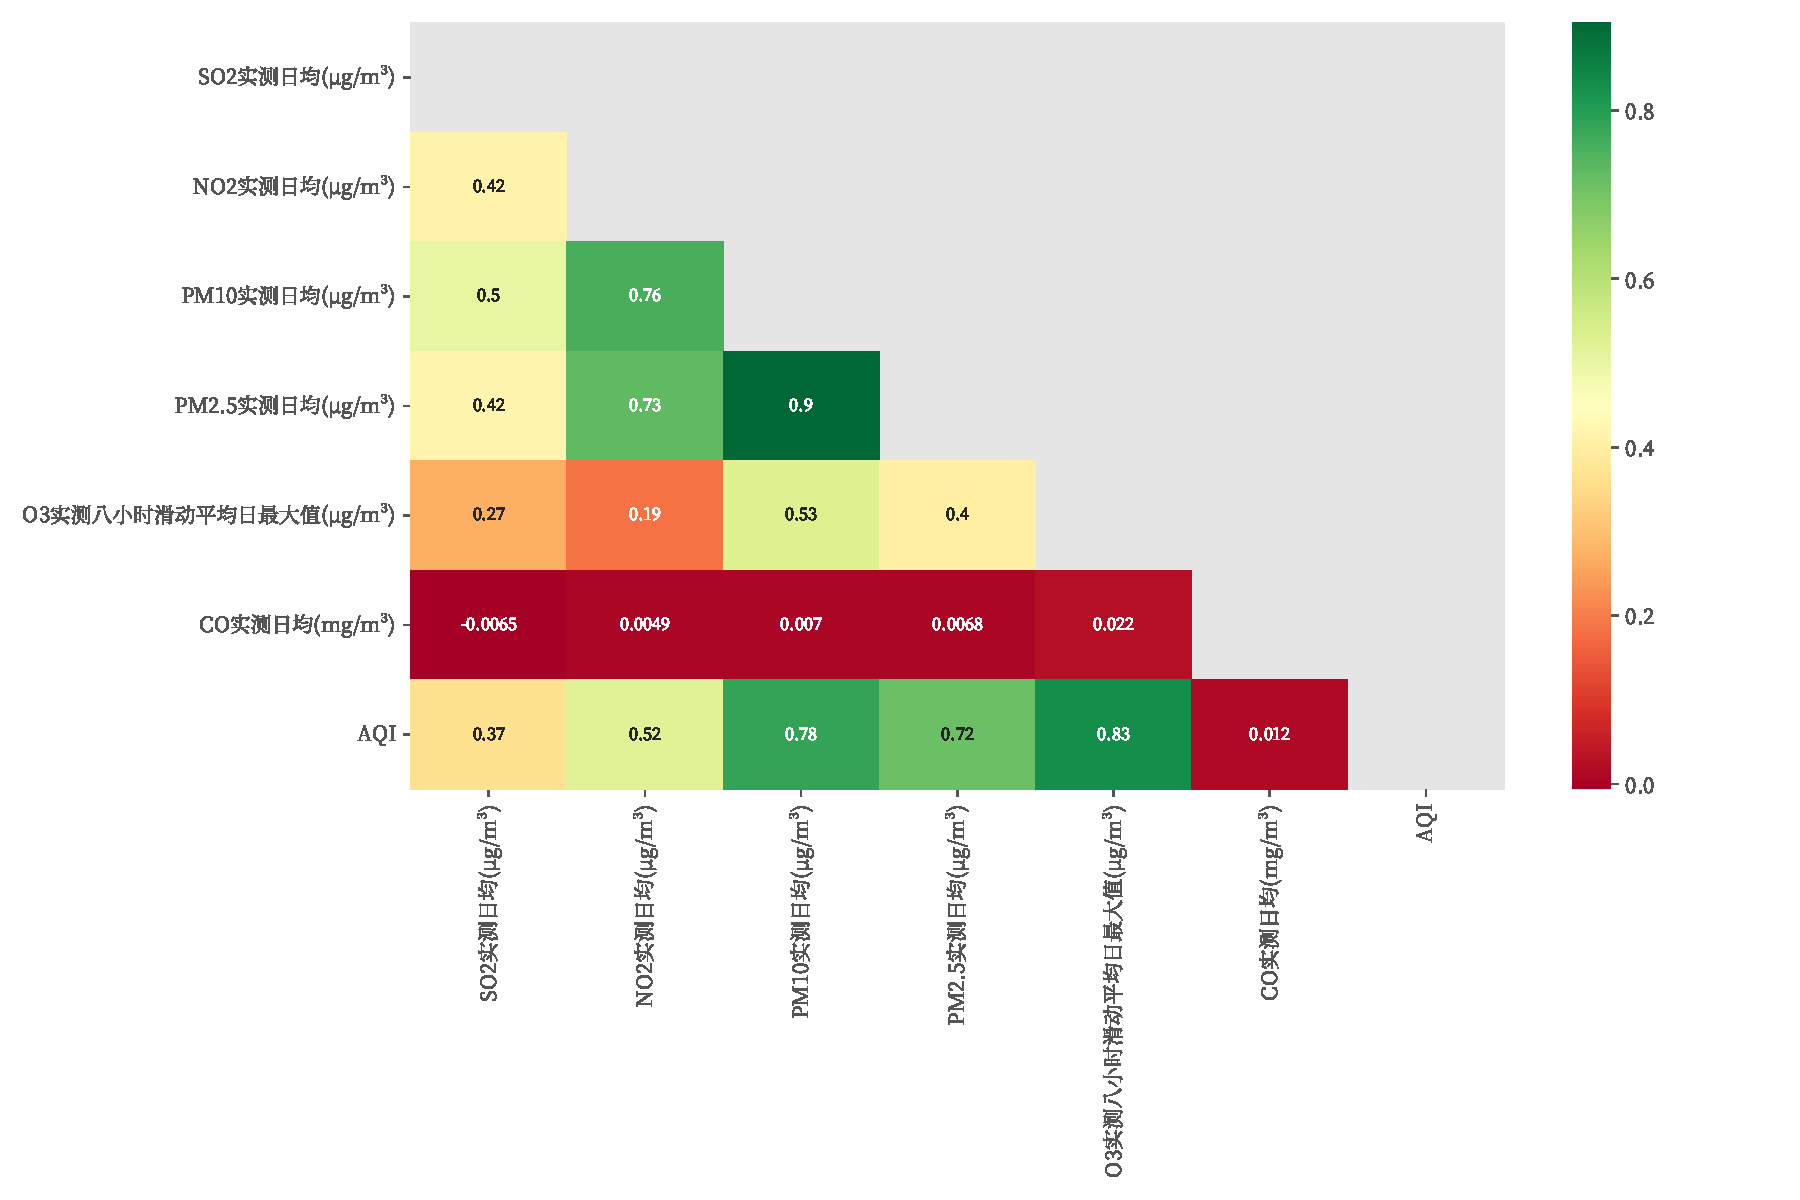
\includegraphics[width=5in]{C-2相关性分析.pdf}
    \end{minipage}}

  }
  \caption{数据异常值量化图}\label{fig_异常值}
\end{figure}



%--------------------问题三的模型建立与求解----------------------
\section{问题三的模型建立与求解}
问题三要求利用附件1和2中的数据,建立一个同时适用于A、B、C三个监测点的二次预报数学模型,三个监测点之间的直线距离大于${100km}$且互不影响,用该模型预测A、B、C三个监测点在2021年7月13日至7月15日这三天的6种常规污染物单日浓度值,要求二次预报模型预测结果中AQI预报值的最大相对误差应尽量小,且首要污染物预测准确度尽量高。

\textbf{已知信息}

问题三提供的数据有三个:

(1) 三个监测点A、B、C的逐小时污染物浓度与气象一次预报数据表;

(2) 三个监测点A、B、C的逐小时污染物浓度与气象实测数据表;

(3) 三个监测点A、B、C的逐日污染物浓度实测数据表。

% 前期空气质量研究多基于2012年以前空气质量检测资料,环保部在2012年发布的环境空气质量标准中加入了${PM_2.5}$以及${O_3-8h}$浓度的质量浓度标准。

% 臭氧${O_3}$又称为超氧,是氧气的同素异形体,大气中的臭氧层可以吸收太阳释放出来的绝大部分紫外线,使人免遭紫外线造成的伤害。然而,超标的地表臭氧会对人体造成伤害,它会强烈刺激人的眼睛和呼吸道,还会造成人的神经中毒,对人体皮肤中的维生素E也会起到破坏作用。因此,测定地标臭氧浓度是否超标必须引起人们的高度重视。{\color{red}[k近邻-吕昊芝]}

% 近地面大气${O_3}$的生成反应主要是由太阳光中的紫外线引起的,所以白天${O_3}$浓度的变化应该与太阳辐射强度存在一定的相关性。{\color{red}图 4 给出了 2012 年 7 月臭氧浓度和太阳辐射的昼间( 7: 00 ~ 18: 00) 变化规律。表2 给出了 2012 年 7 月小时平均太阳辐射强度昼间( 7∶ 00~ 18∶ 00) 和 ${O_3}$浓度变化情况。}从图中可以看出,${O_3}$浓度随着太阳辐射强度的变化而变化,二者变化趋势基本一致,${O_3}$浓度的最值滞后于太阳辐射强度最值约 2小时。由表 2 可以得到臭氧浓度值与同时段的太阳辐射强度的相关系数 R 为 0. 336,这说明 ${O_3}$浓度值受同时段的太阳辐射强度影响不大,但是考虑到太阳辐射强度引起的环境空气中 ${O_3}$浓度监测结果滞后于辐射强度本身的变化,我们将每日 9 时到 20 时的 ${O_3}$浓度与 7 时到18 时 的 太 阳 辐 射 强 度 相 对 应, 求 得 其 相 关 系 数 为0. 7276,由此可见,${O_3}$浓度值受与其相对应的前 2 个小时的太阳辐射强度影响较大。{\color{red}[姜峰-夏季城市臭氧\dots]}

% 国内外的许多专家投身于对该指标的分析和预测中,臭氧日一词随之诞生,本文选用臭氧八小时作为臭氧日污染衡量标准,即一天中臭氧最高的连续8小时的平均浓度值。相较于过去落后的针对空气质量的人工推算,利用机器学习分析大气问题可以极大提高预测的准确率,同时也可以缩短分析预测所需时间,从而保证空气质量预报的时效性,因此该研究具有极其深刻的现实意义。{\color{red}[k近邻-吕昊芝]}

% 近年来随着经济的发展、人口的激增以及机动车保有量的增加,我国城市臭氧(${O_3}$) 污染问题愈发严重( Wang et al.,2016)。为全面认识${O_3}$的污染规律,国内外学者在${O_3}$的光化学反应( An et al.,2015) 、来源敏感性分析(Zhang et al.,2014; 李浩等,2015) 、人体健康效应、区域传输作用等方面开展了研究,探讨气象因素( Mohd et al.,2016) 、植被覆盖( Fu et al.,2015) 、土地利用等( Wolf et al.,2016) 对${O_3}$的影响,分析典型污染过程和重大历史事件的污染规律。此外,不少学者还使用了统计模型来研究${O_3}$的时空分布特征和影响因素。洪盛茂等( 2009) 运用多元非线性回归分析了杭州地区${O_3}$浓度与天气系统等因素的相关性; 沈路路等(2011) 运用神经网络模型研究了气象因素对${O_3}$的驱动作用; 程麟钧等( 2017) 基于旋转经验正交函数法(REOF) 对中国${O_3}$时空分布特征进行了研究,发现地形和地貌对臭氧空间相关性具有重要影响; 李霄阳等(2018) 运用空间自相关方法分析了2016年中国城市${O_3}$污染的空间集聚和冷热点区域的时空特征; Wolf 等(2017)运用土地利用回归模型研究${O_3}$影响因素及空间分布特征。{\color{red}[胡成媛-基于GAM模型的四川盆地]\dots}

% 尽管已有研究从${O_3}$前体物排放、气象环境因素、化学反应过程等方面,应用旋转经验正交函数分解法、土地利用回归、地理加权回归、空间自相关等方法分析了${O_3}$浓度时空变化的影响因素,但只考虑了${O_3}$浓度与影响因素的线性相关关系却忽略了不同变量间复杂的非线性关系。目前,运用非线性模型分析影响因素对${O_3}$浓度变化的研究成果还非常少,综合考虑影响因素交互作用对${O_3}$浓度变化影响的研究成果则更是鲜有报道。${O_3}$浓度与空气污染物、气象要素等影响因素构成了一个复杂的非线性动力系统,因素之间存在强烈的反馈与调节的非线性相互作用,其时间序列也反映了${O_3}$浓度与影响因素间线性与非线性相互作用与发展变化过程。广义相加模型(Generalized Additive Model,GAM) 是广义线性模型和可加模型的结合形式,可用于响应变量与解释变量之间的关系是非线性和非单调的数据分析,目前已被广泛应用于处理复杂的非线性空气污染问题。贺祥等( 2017) 基于GAM模型分析了影响因素交互作用对南京市PM2.5浓度变化的影响,结果表明影响因素交互作用对 PM2.5浓度变化解释率较高,其中${SO_2}$与 CO、气压和相对湿度的交互作用对PM2.5浓度变化具有显著影响。 Gong 等(2017) 利用GAM 模型量化了气象条件对美国中部地区臭氧污染的影响,指出GAM模型能较高地预测因气象要素和局地传输条件的变化所导致的${O_3}$浓度变化。{\color{red}[胡成媛-基于GAM模型的四川盆地]\dots}

% {\color{red}如果利用GAM模型}

% {\color{red}[检验模型预测的指标!!!]}

% {\color{blue}1.压轴回归法(RMA) 2.相关性矩阵}

\subsection{问题的描述分析}
因为题目中说A、B、C三个站点之间的影响可以忽略,但气象条件中包含了风向等受地理位置影响的解释变量,所以不能直接将此类的数据直接用于预测模型的构建,需要将此类的解释变量进行剔除,再进行其他分析。本文首先对解释变量进行了\textbf{预分析},剔除掉对地理位置有影响的变量以及存在共线性的变量,\textbf{降低多重共线性}对模型的影响。预分析之后进行一个\textbf{并行处理},第一步分别将6项污染物作为响应变量,每次选取剩余的影响因素中的一项作为解释变量,进行\textbf{广义相加模型}(Generalized Additive Model, GAM)分析\textsuperscript{\cite{ref5}},并行步则是分别将6项污染物作为响应变量,与所有的预分析后的影响因素进行GAM模型分析,综合并行处理的结果,选取出对6项污染物浓度变化解释率等较高的气象条件作为预测模型的变量,将最终选定的多项解释变量送入GAM模型,完成最终污染物浓度的预测模型的搭建。

% 本文首先绘制出了原始数据中21个变量的频率直方图及密度分布曲线,如图7.1所示,从图中数据可以看出,数据整体基本符合正态分布类型,

多重共线性是指线性回归模型中的解释变量之间存在高度相关关系而使模型估计失真或难以准确估计\textsuperscript{\cite{ref6}}。本文采用皮尔斯相关系数来判别解释变量之间是否存在的共线性,如果解释变量间相关系数较大,则两个解释变量之间通常存在严重共曲线性关系,需要剔除一个解释变量,用留下的解释变量指标来代表丢弃变量指标。

GAM是一种非参数回归模型,模型中部分或全部的自变量采用平滑函数,以此来降低线性拟合带来的风险,属于组合模型。该模型不需要预假设模型中自变量是否线性相关于因变量,对于模型的假定比较宽松,可以解决Logistic回归多解释变量时引发的维度灾难问题。

\subsection{数学模型的建立}
本文首先对数据进行了预分析,得到了解释变量自身的频率分布直方图与密度分布曲线,如图\ref{fig_Histogram}所示,从图中可以看出,21个解释变量基本符合正态分布类型,其中,近地2米温度和地表温度的数据分布走向基本类似,比湿与湿度的主要数据分布基本类似,考虑到题目中所说的A、B、C三个监测点之间的影响忽略不计,需要剔除近地风向这一影响因素。

\begin{figure}[!htbp]
    \center{
    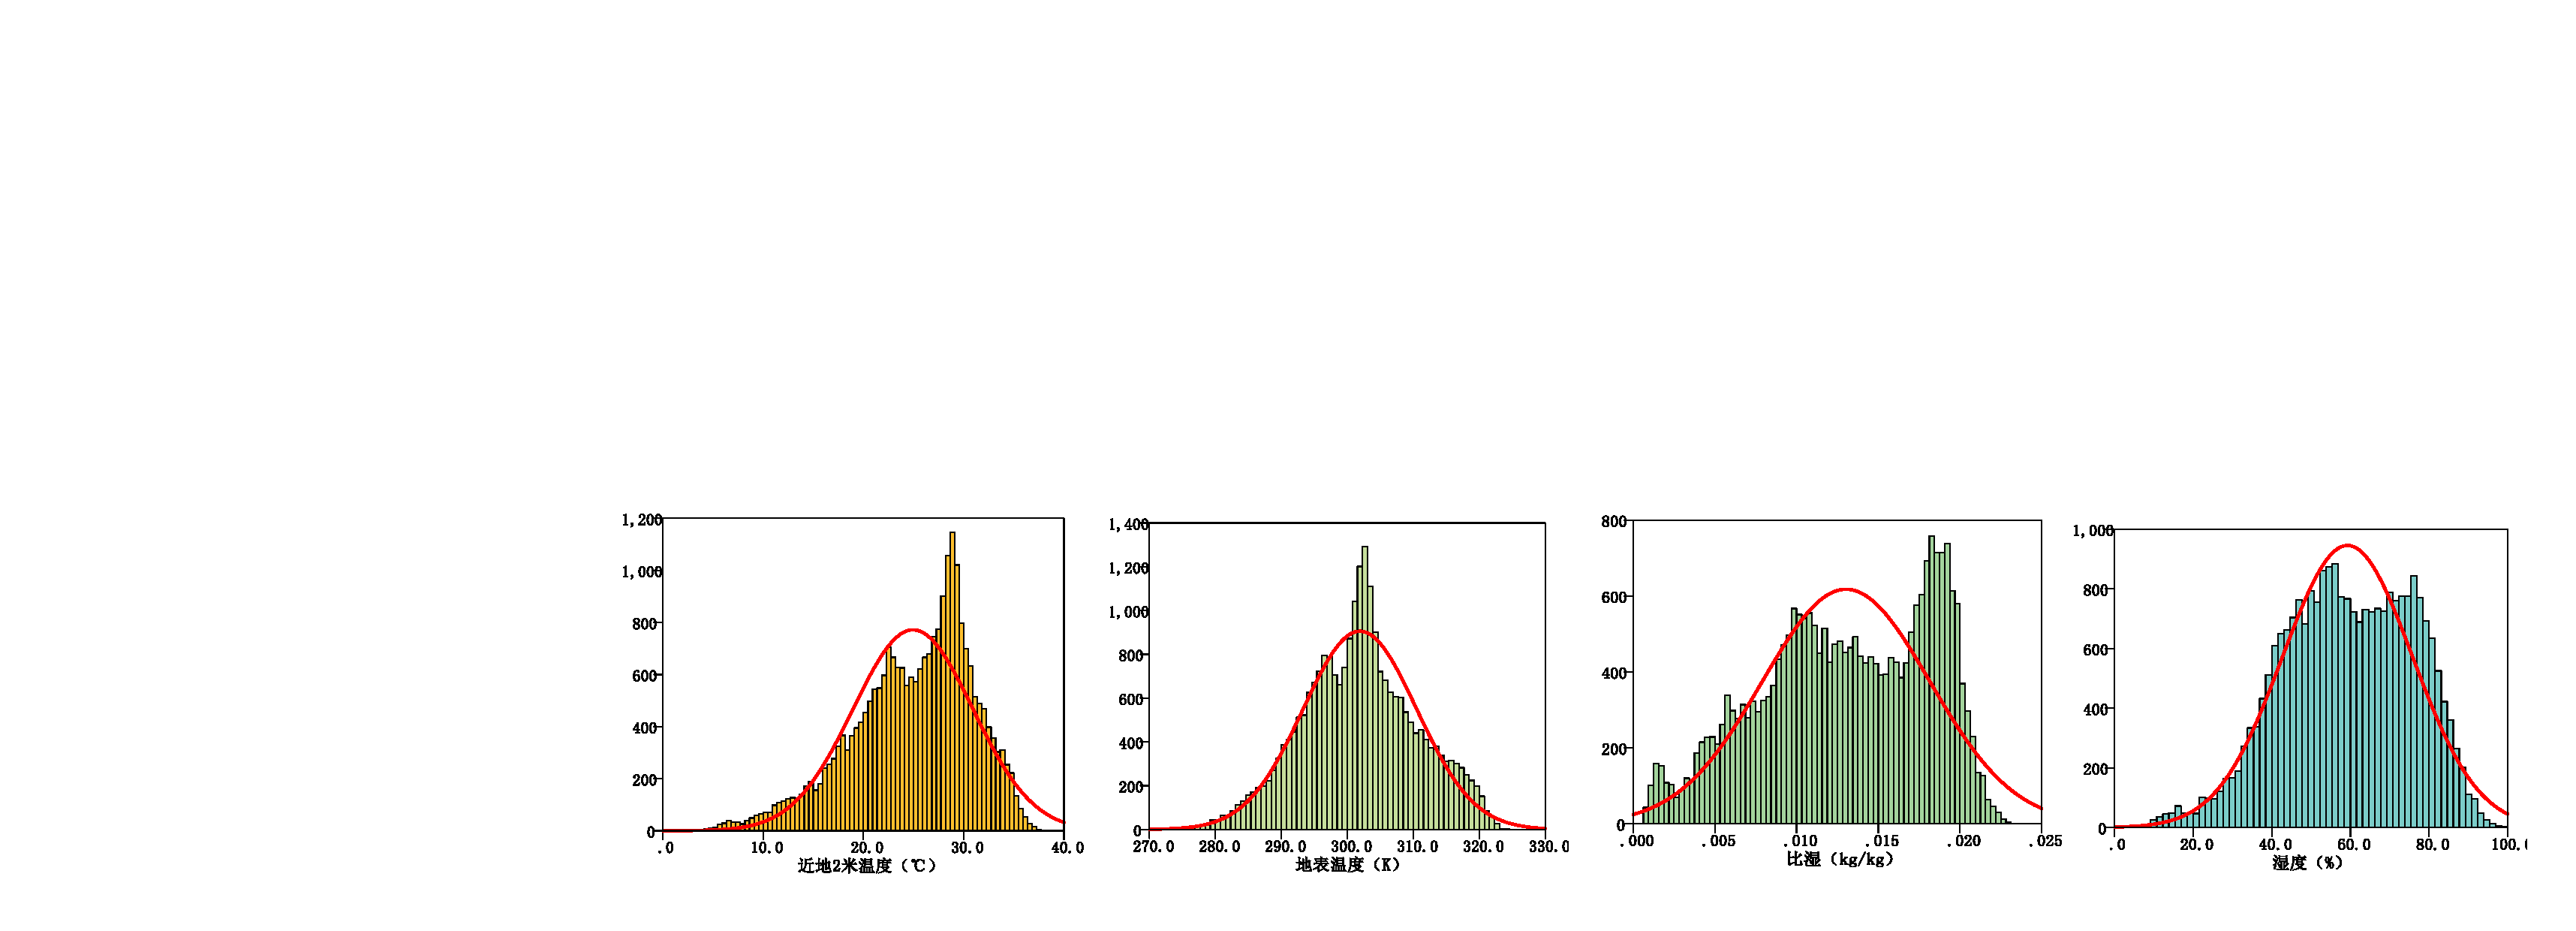
\includegraphics[width=.9\textwidth]{Sig_Histogram_1.pdf}\\
    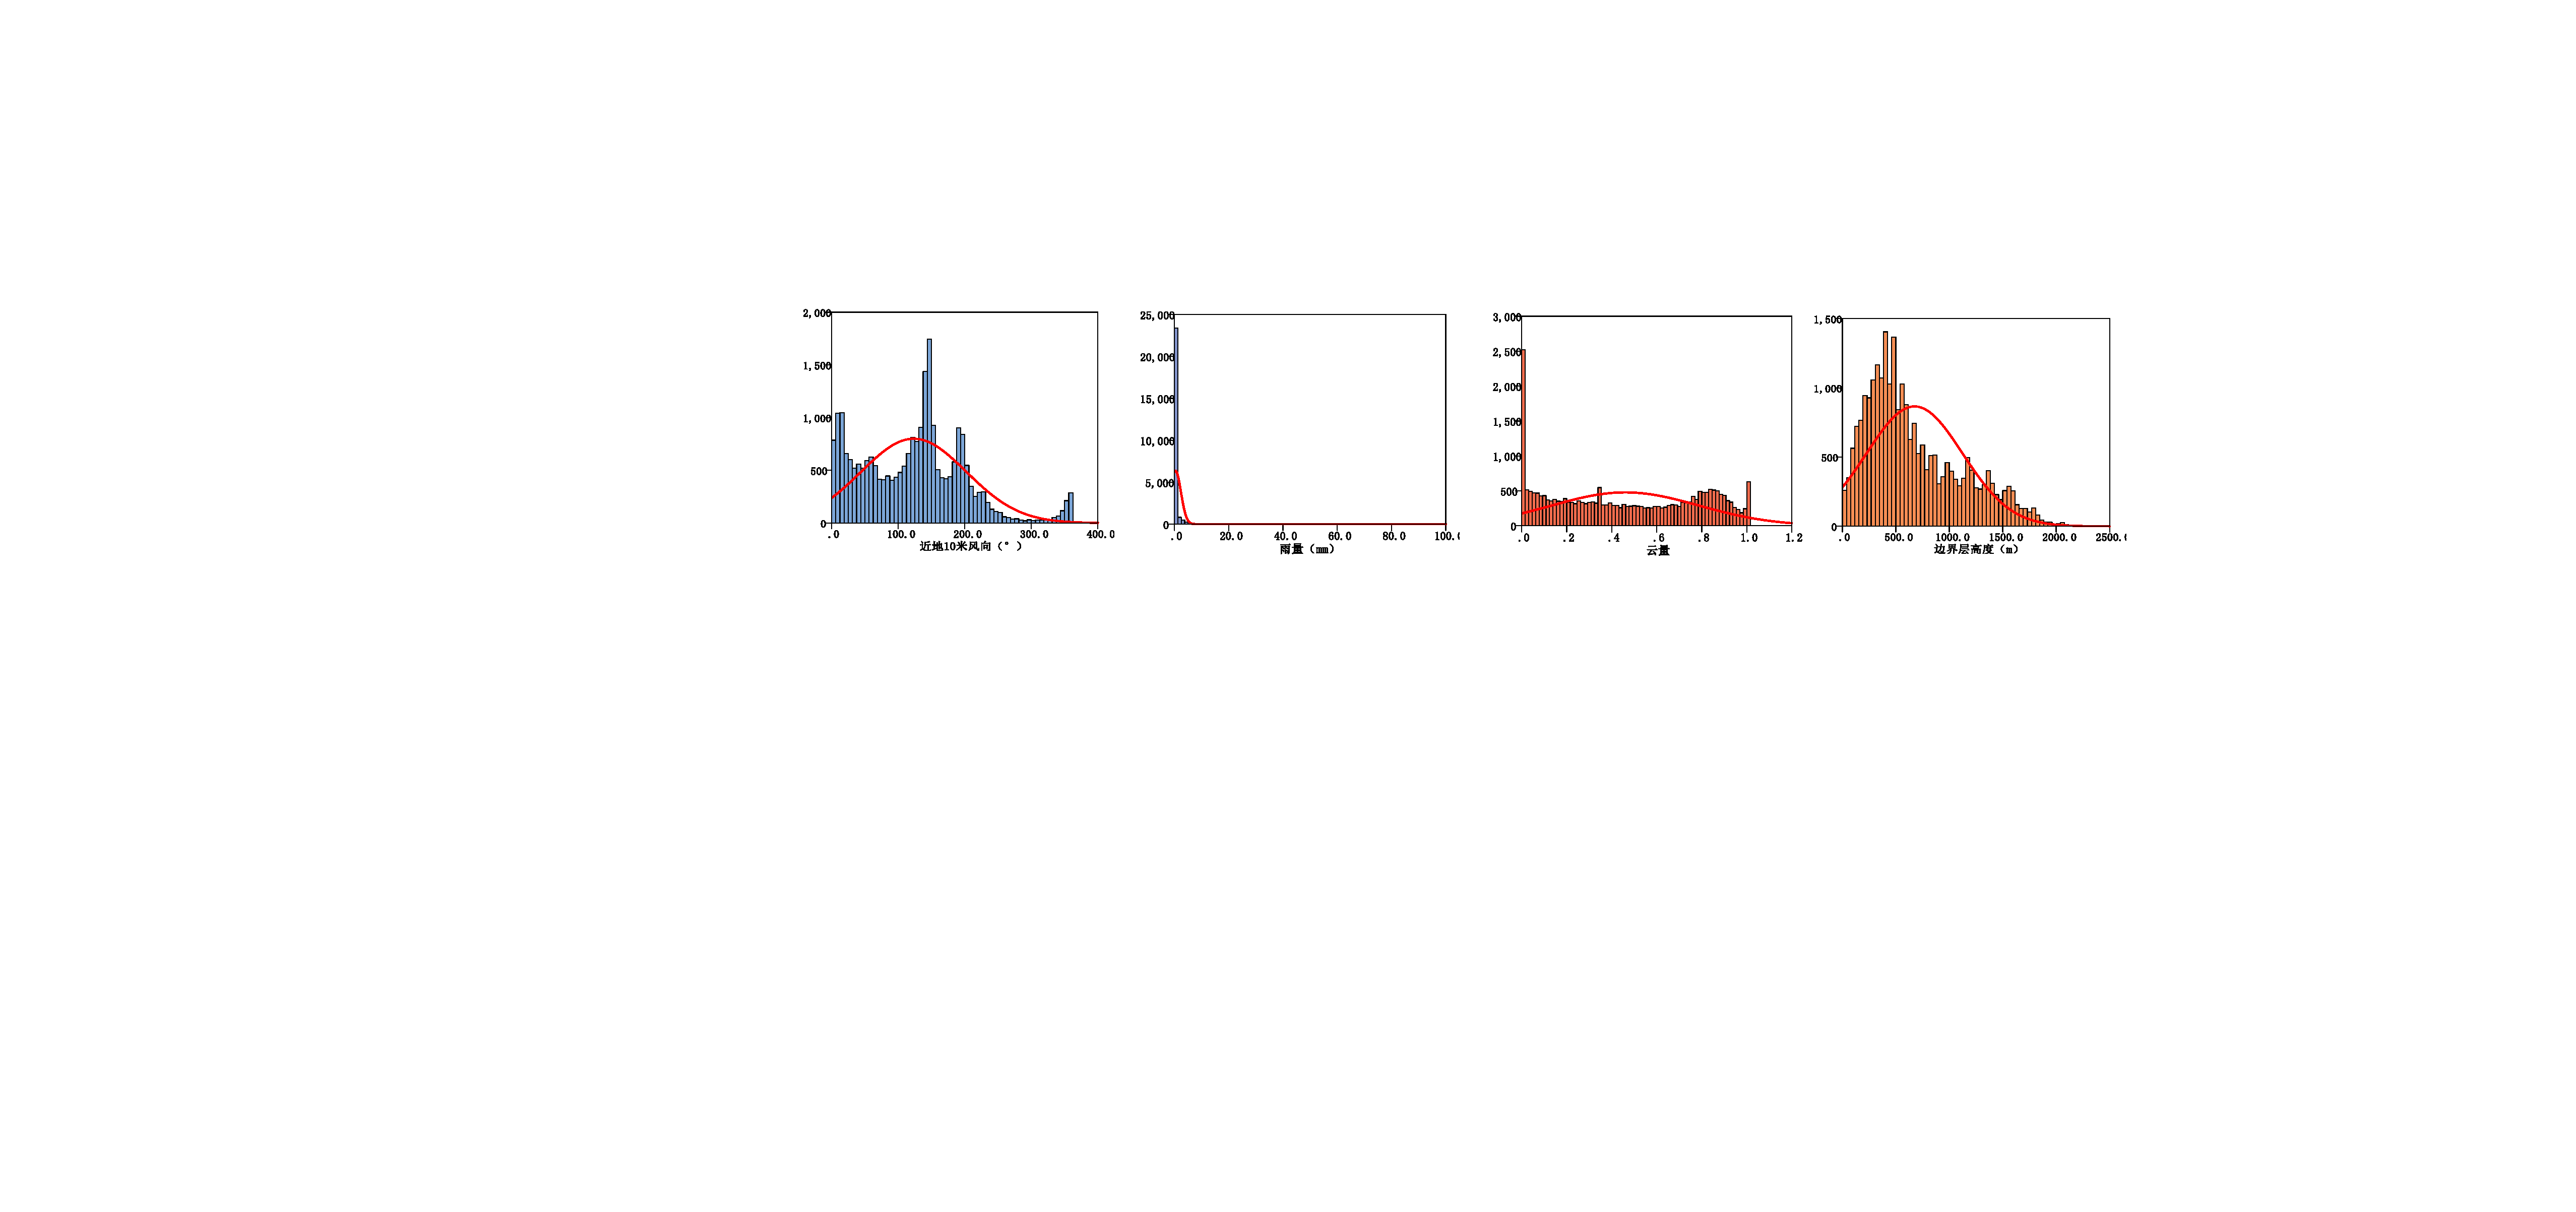
\includegraphics[width=.9\textwidth]{Sig_Histogram_2.pdf}\\
    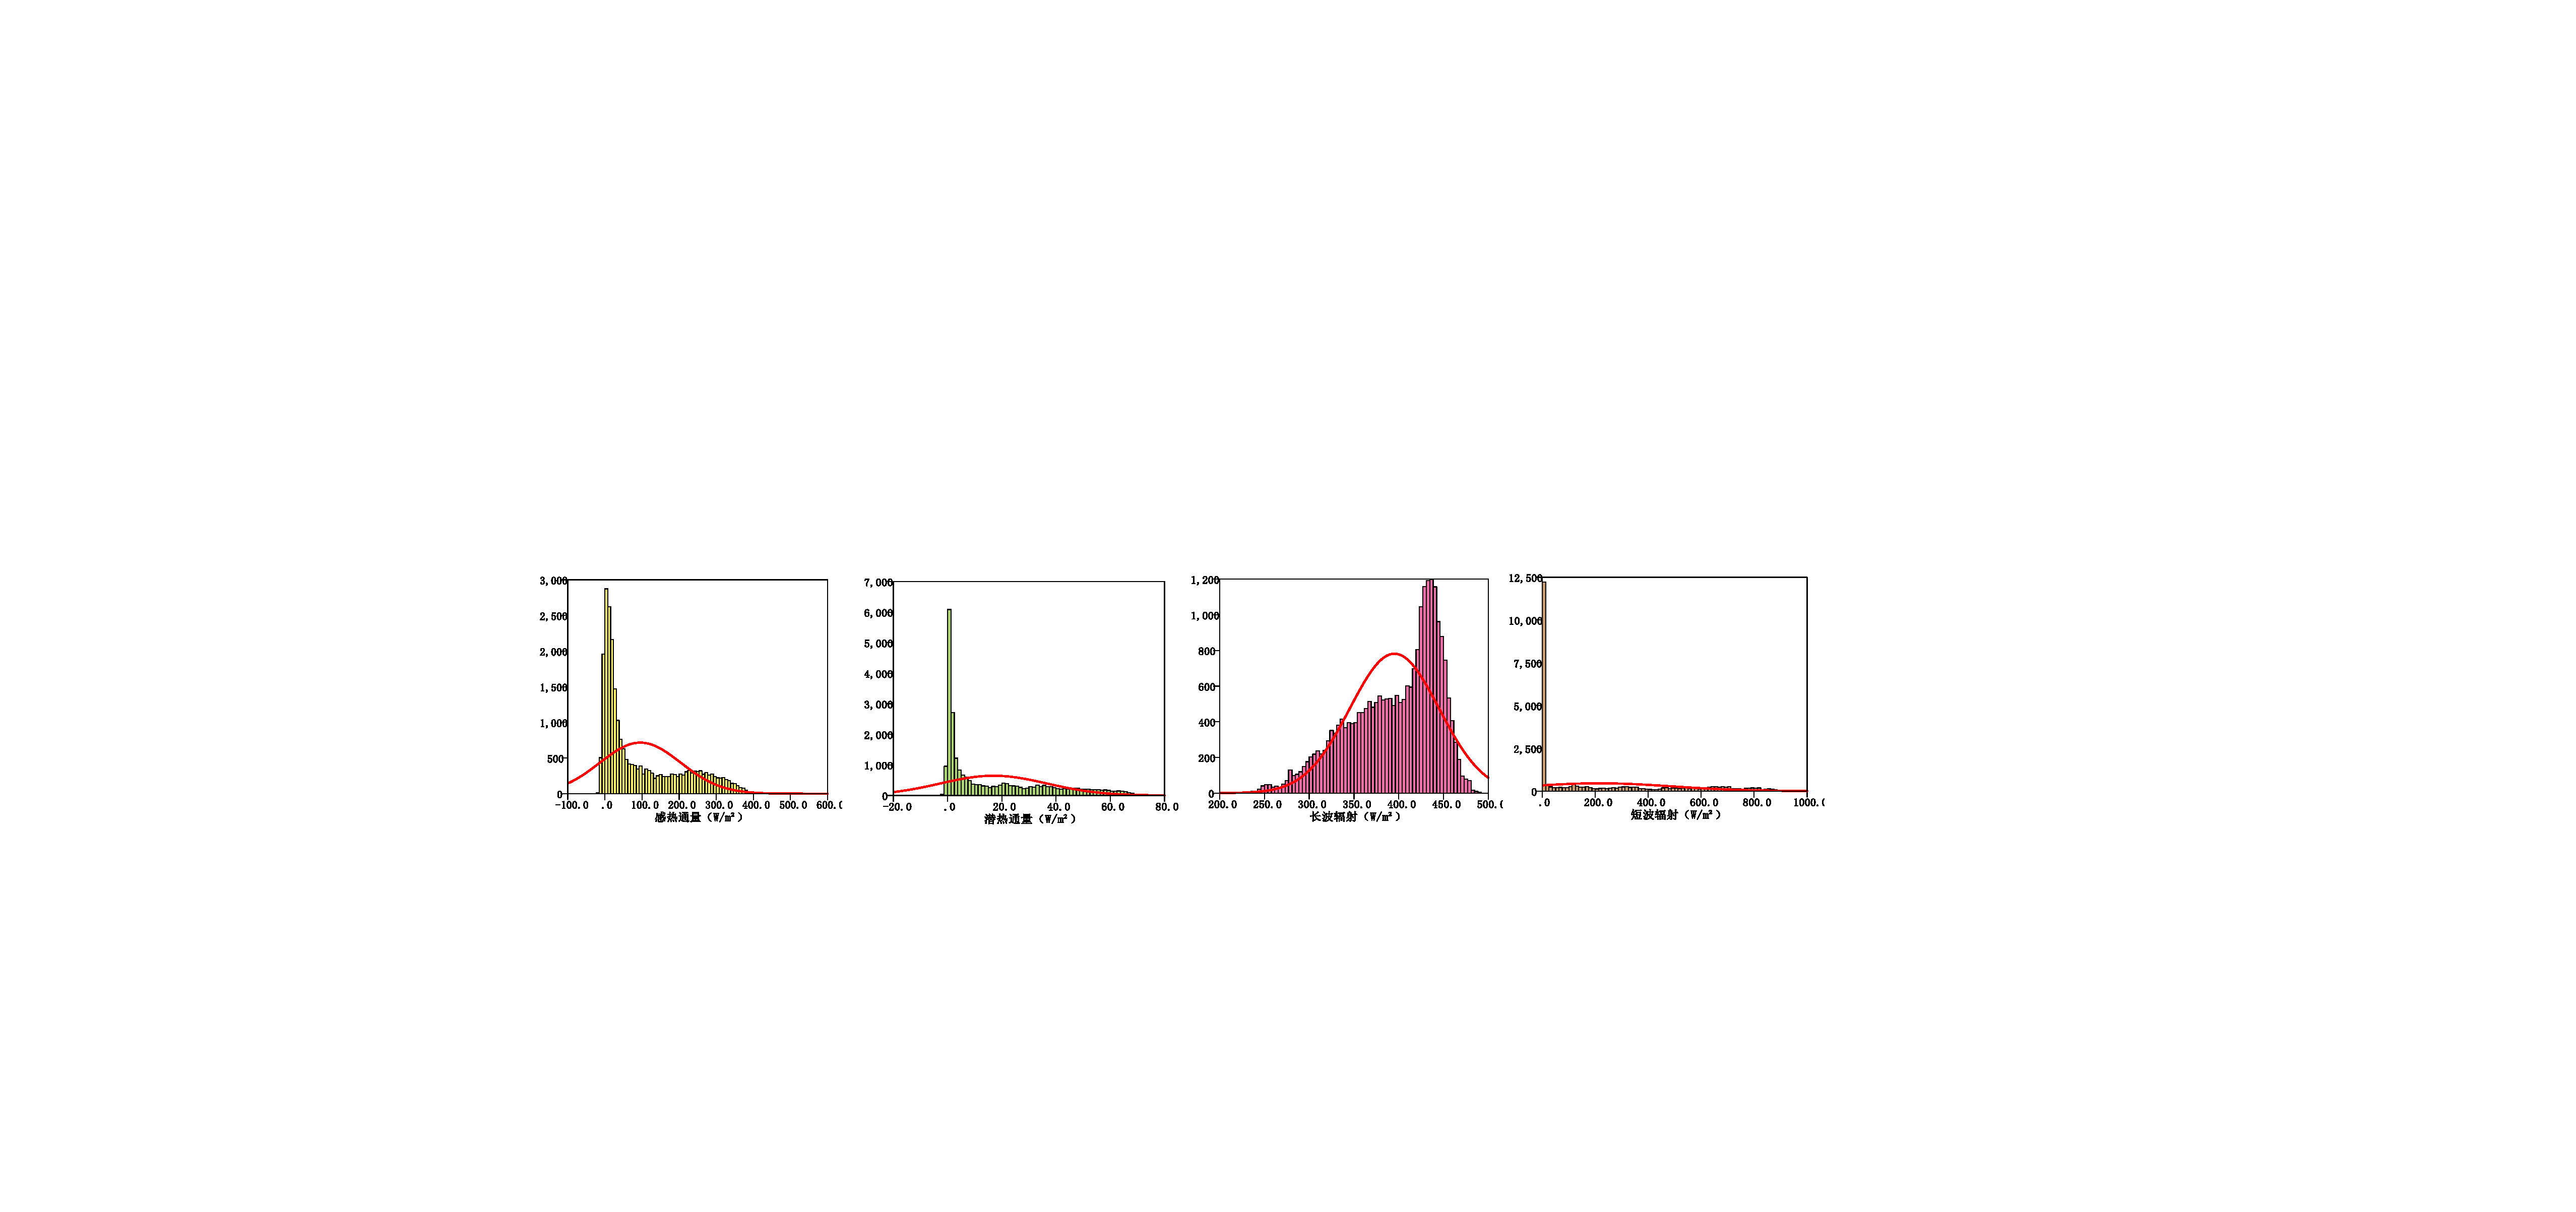
\includegraphics[width=.9\textwidth]{Sig_Histogram_3.pdf}\\
    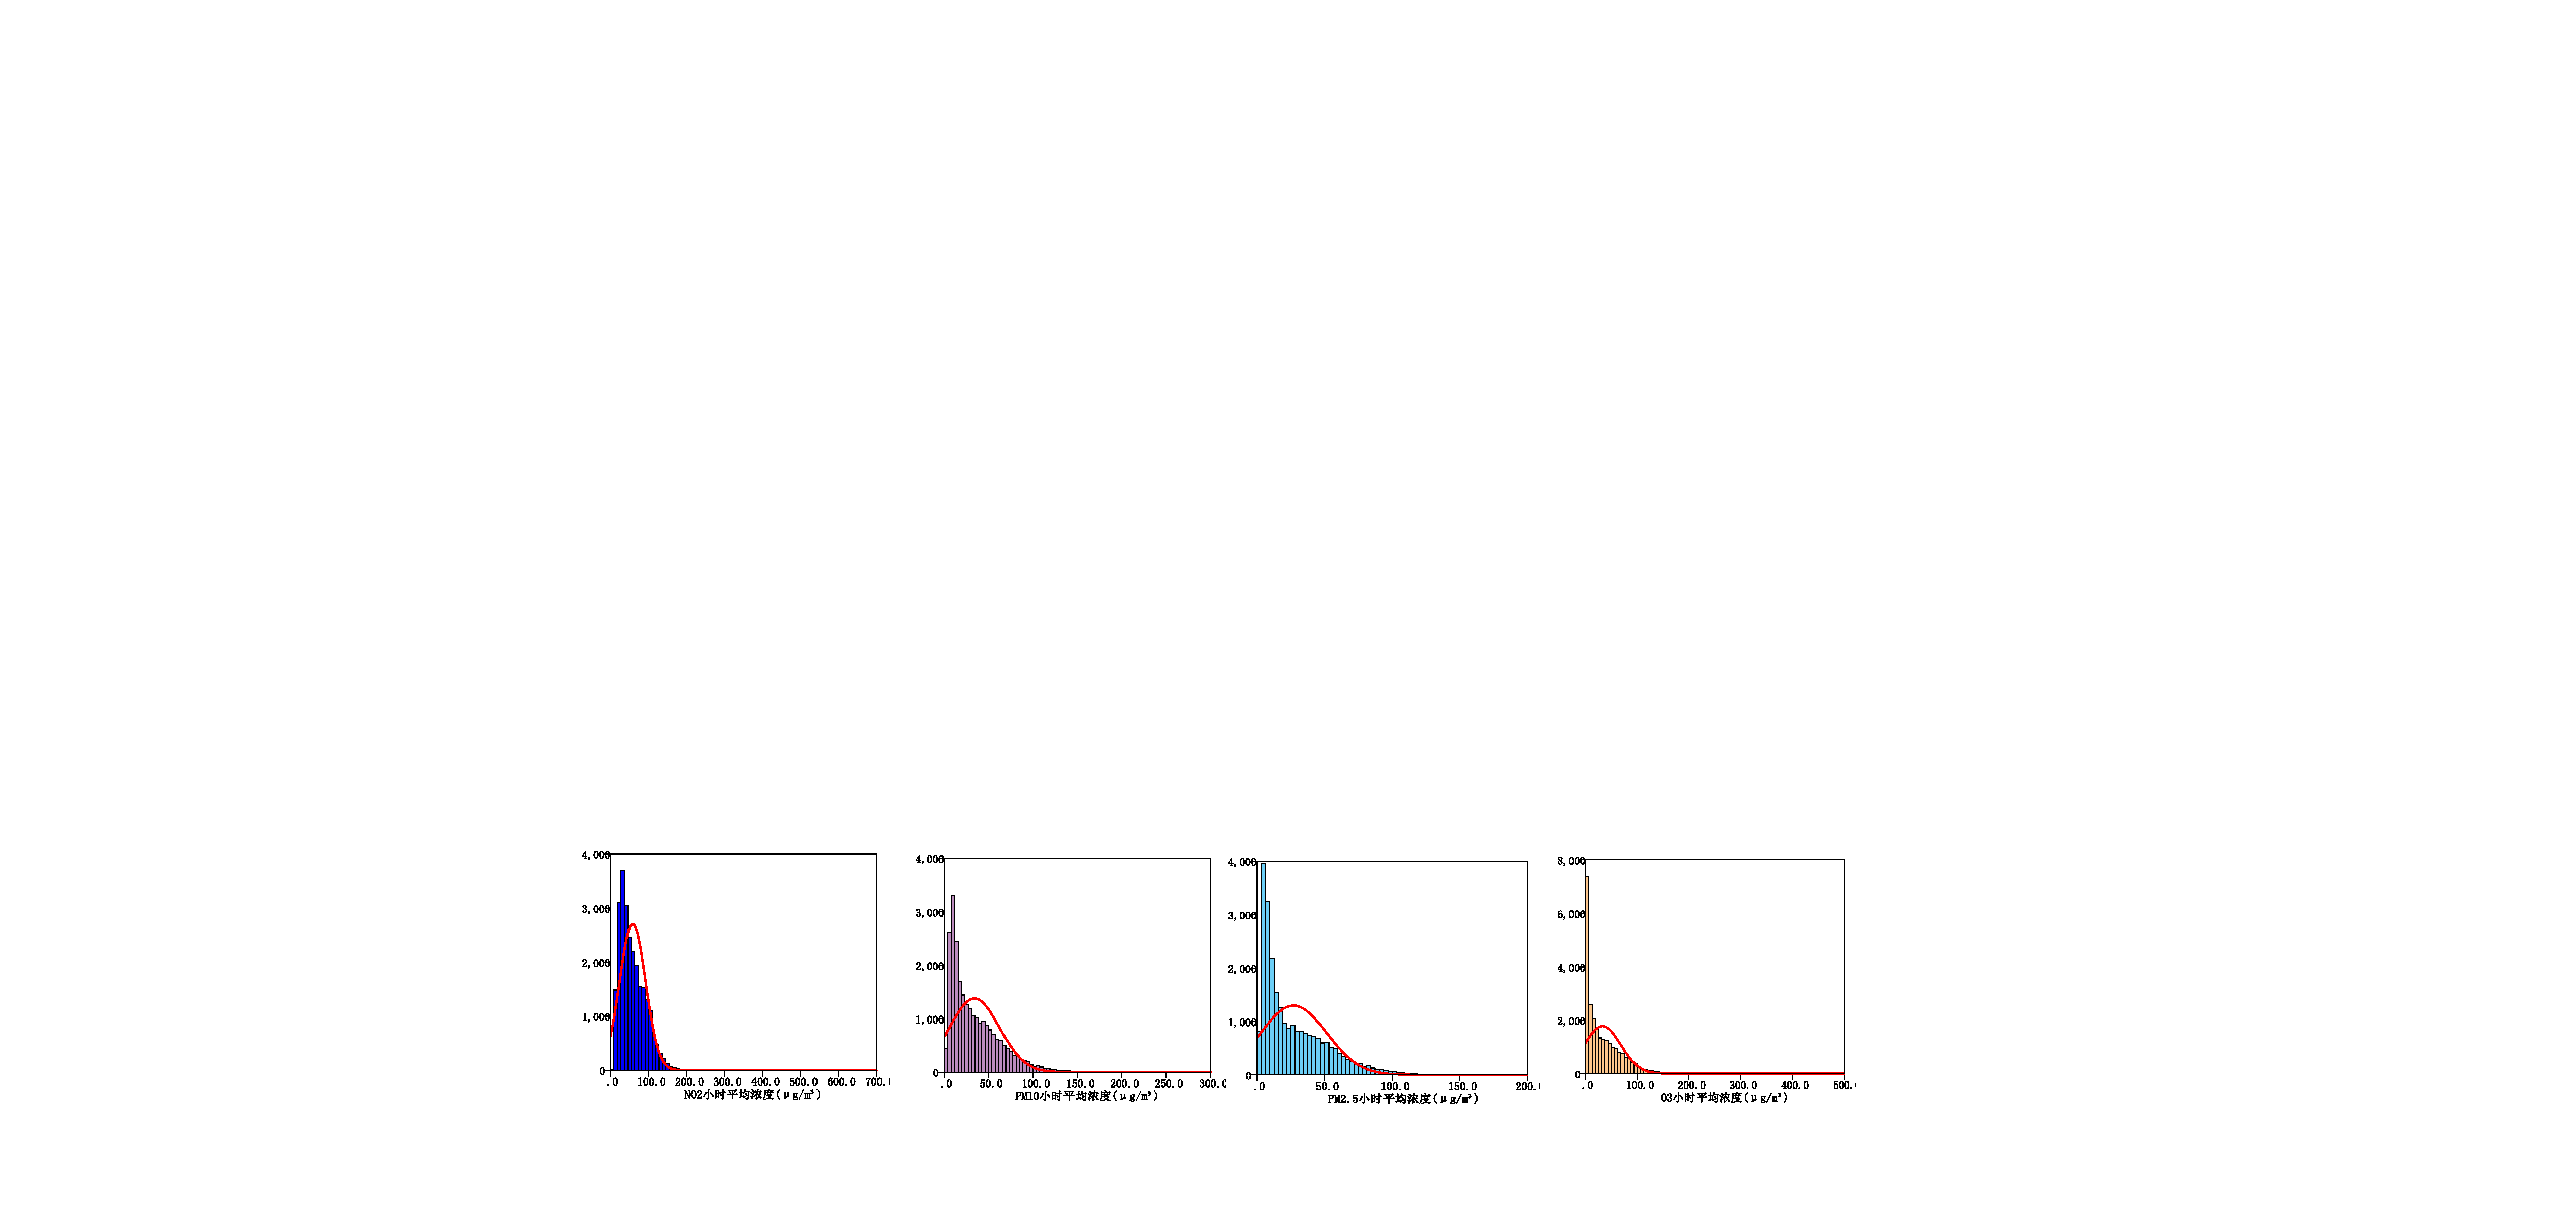
\includegraphics[width=.9\textwidth]{Sig_Histogram_4.pdf}\\
    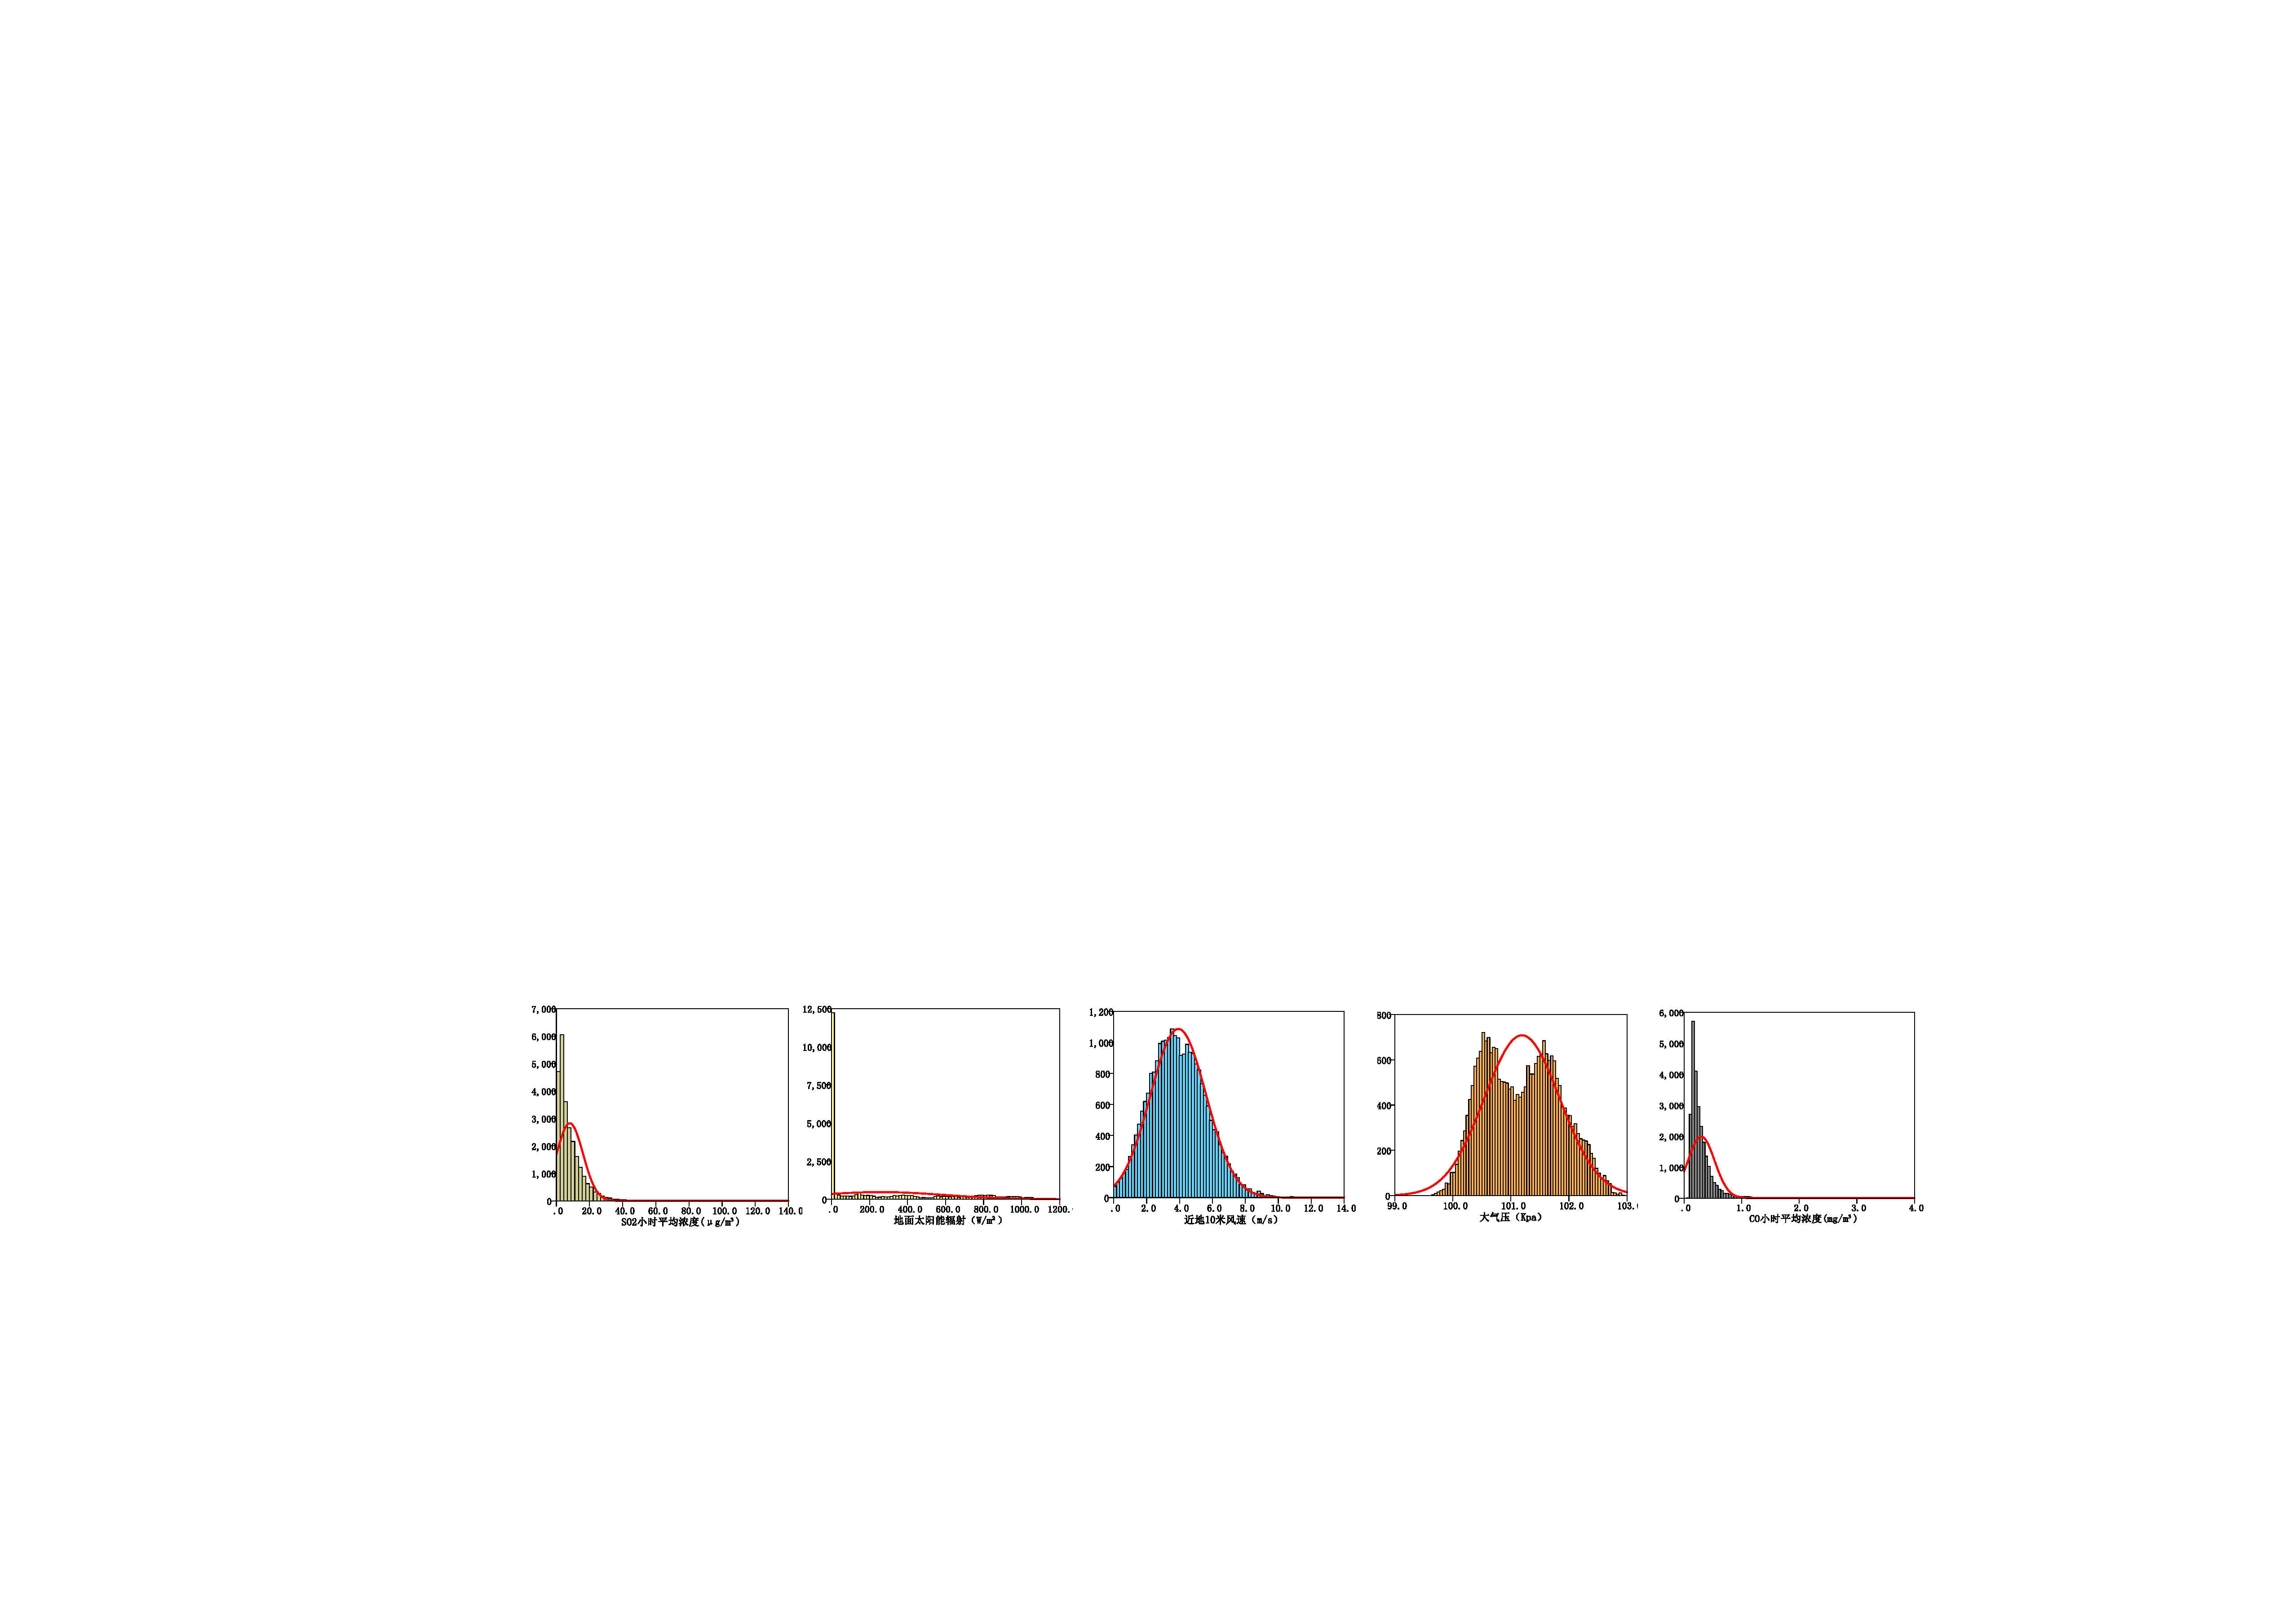
\includegraphics[width=.9\textwidth]{Sig_Histogram_5.pdf}
    }
    \caption{影响因素的频率分布直方图与密度分布曲线}\label{fig_Histogram}
\end{figure}

\subsubsection{解释变量预分析}
为了更进一步量化解释变量之间的相关性,本文采用了双变量的Pearson相关系数分析,结果如表\ref{tab_person}所示,从表中数据可以看到,近地2米温度与地表温度、长波辐射,长波辐射与比湿,潜热通量与感热通量、短波辐射、地面太阳能辐射,短波辐射与感热通量、潜热通量、地面太阳能辐射,感热通量与地面太阳能辐射之间的相关系数均在${85\%}$以上,在${P<0.05}$和${P<0.01}$上显著相关,而所有的数值中,短波辐射和地面太阳能辐射之间相关系数最高,从概率分布直方图和密度分布曲线也可以看出,两个影响因素具有极高的共线性,那是因为太阳辐射波长较地面和大气辐射波长小得多,所以通常又称太阳辐射为短波辐射,因此在计算相关系数时,呈现了高度的互相关性,考虑到太阳能辐射与其他几个也呈现了较高的相关性,于是本文舍弃掉了太阳能辐射这一变量,采用其他的标量指标来代替太阳能辐射,以此减少构建多变量曲线模型能产生的解释变量共曲线性问题。

% Table generated by Excel2LaTeX from sheet 'Sheet1'
\begin{sidewaystable}[htbp]
\scriptsize
    \centering
    \caption{影响因素间Person相关系数}\label{tab_person}%
    \begin{threeparttable}
      \begin{tabular}{p{2.5em}ccccccccccccccccccccc}
      \toprule
      \multicolumn{1}{c}{} & \multicolumn{1}{p{2.165em}}{\textbf{T\_2}} & \multicolumn{1}{p{1.89em}}{\textbf{T}} & \multicolumn{1}{p{3.61em}}{\textbf{R\_Hu}} & \multicolumn{1}{p{1.89em}}{\textbf{Hu}} & \multicolumn{1}{p{3.165em}}{\textbf{Win\_S}} & \multicolumn{1}{p{3.72em}}{\textbf{Win\_D}} & \multicolumn{1}{p{2.055em}}{\textbf{Rain}} & \multicolumn{1}{p{2.39em}}{\textbf{Cloud}} & \multicolumn{1}{p{3.72em}}{\textbf{High\_B}} & \multicolumn{1}{p{2.945em}}{\textbf{Atmos}} & \multicolumn{1}{p{3.335em}}{\textbf{Sen\_H}} & \multicolumn{1}{p{2.835em}}{\textbf{Lat\_H}} & \multicolumn{1}{p{2.835em}}{\textbf{Long\_W}} & \multicolumn{1}{p{2.89em}}{\textbf{Short\_W}} & \multicolumn{1}{p{3.665em}}{\textbf{Solar\_R}} & \multicolumn{1}{p{1.89em}}{\textbf{SO2}} & \multicolumn{1}{p{1.89em}}{\textbf{NO2}} & \multicolumn{1}{p{1.89em}}{\textbf{PM10}} & \multicolumn{1}{p{1.89em}}{\textbf{PM2.5}} & \multicolumn{1}{p{1.89em}}{\textbf{O3}} & \multicolumn{1}{p{1.89em}}{\textbf{CO}} \\
      \midrule
      \textbf{T\_2} & \textcolor[rgb]{ .004,  .008,  .02}{1} & \textcolor[rgb]{ 1,  0,  0}{\textbf{.901**}} & .790** & .077** & .102** & .389** & .105** & -.026** & .493** & -.867** & .366** & .449** & \textcolor[rgb]{ 1,  0,  0}{\textbf{.858**}} & .320** & .320** & -.469** & -.515** & -.632** & -.626** & .184** & -.330** \\
      \textbf{T} & \textcolor[rgb]{ 1,  0,  0}{\textbf{.901**}} & \textcolor[rgb]{ .004,  .008,  .02}{1} & .581** & -.142** & .069** & .307** & .094** & -.116** & .711** & -.700** & .710** & .769** & .693** & .686** & .686** & -.441** & -.490** & -.553** & -.529** & .431** & -.309** \\
      \textbf{R\_Hu} & .790** & .581** & \textcolor[rgb]{ .004,  .008,  .02}{1} & .607** & -.024** & .428** & .208** & .136** & .013* & -.871** & \textcolor[rgb]{ .004,  .008,  .02}{-0.009} & .082** & \textcolor[rgb]{ 1,  0,  0}{\textbf{.859**}} & -.021** & -.021** & -.537** & -.574** & -.671** & -.693** & -.039** & -.364** \\
      \textbf{Hu} & .077** & -.142** & .607** & \textcolor[rgb]{ .004,  .008,  .02}{1} & -.232** & .193** & .173** & .254** & -.568** & -.295** & -.460** & -.407** & .329** & -.417** & -.417** & -.252** & -.196** & -.241** & -.299** & -.245** & -.089** \\
      \textbf{Win\_S} & .102** & .069** & -.024** & -.232** & \textcolor[rgb]{ .004,  .008,  .02}{1} & -.134** & \textcolor[rgb]{ .004,  .008,  .02}{-0.010} & .028** & .220** & -.037** & .157** & .095** & .102** & .036** & .036** & -.132** & -.293** & -.208** & -.155** & \textcolor[rgb]{ .004,  .008,  .02}{-0.004} & -.259** \\
      \textbf{Win\_D} & .389** & .307** & .428** & .193** & -.134** & \textcolor[rgb]{ .004,  .008,  .02}{1} & .049** & -.127** & .059** & -.470** & .049** & .068** & .327** & .019** & .019** & -.352** & -.288** & -.318** & -.363** & .023** & -.168** \\
      \textbf{Rain} & .105** & .094** & .208** & .173** & \textcolor[rgb]{ .004,  .008,  .02}{-0.010} & .049** & \textcolor[rgb]{ .004,  .008,  .02}{1} & .176** & -.063** & -.182** & .021** & .032** & .202** & \textcolor[rgb]{ .004,  .008,  .02}{-0.012} & \textcolor[rgb]{ .004,  .008,  .02}{-0.012} & -.139** & -.109** & -.176** & -.168** & -.027** & -.084** \\
      \textbf{Cloud} & -.026** & -.116** & .136** & .254** & .028** & -.127** & .176** & \textcolor[rgb]{ .004,  .008,  .02}{1} & -.231** & -.045** & -.245** & -.207** & .348** & -.258** & -.258** & \textcolor[rgb]{ .004,  .008,  .02}{0.007} & \textcolor[rgb]{ .004,  .008,  .02}{0.010} & -.072** & -.060** & -.125** & \textcolor[rgb]{ .004,  .008,  .02}{0.002} \\
      \textbf{High\_B} & .493** & .711** & .013* & -.568** & .220** & .059** & -.063** & -.231** & \textcolor[rgb]{ .004,  .008,  .02}{1} & -.218** & .781** & .775** & .230** & .713** & .713** & -.208** & -.217** & -.211** & -.164** & .460** & -.171** \\
      \textbf{Atmos} & -.867** & -.700** & -.871** & -.295** & -.037** & -.470** & -.182** & -.045** & -.218** & \textcolor[rgb]{ .004,  .008,  .02}{1} & -.149** & -.234** & -.835** & -.103** & -.103** & .493** & .522** & .647** & .659** & -.013* & .333** \\
      \textbf{Sen\_H} & .366** & .710** & \textcolor[rgb]{ .004,  .008,  .02}{-0.009} & -.460** & .157** & .049** & .021** & -.245** & .781** & -.149** & \textcolor[rgb]{ .004,  .008,  .02}{1} & \textcolor[rgb]{ 1,  0,  0}{\textbf{.965**}} & .121** & \textcolor[rgb]{ 1,  0,  0}{\textbf{.957**}} & \textcolor[rgb]{ 1,  0,  0}{\textbf{.957**}} & -.201** & -.267** & -.182** & -.143** & .583** & -.156** \\
      \textbf{Lat\_H} & .449** & .769** & .082** & -.407** & .095** & .068** & .032** & -.207** & .775** & -.234** & \textcolor[rgb]{ 1,  0,  0}{\textbf{.965**}} & \textcolor[rgb]{ .004,  .008,  .02}{1} & .218** & \textcolor[rgb]{ 1,  0,  0}{\textbf{.965**}} & \textcolor[rgb]{ 1,  0,  0}{\textbf{.965**}} & -.223** & -.296** & -.228** & -.191** & .592** & -.170** \\
      \textbf{Long\_W} & \textcolor[rgb]{ 1,  0,  0}{\textbf{.858**}} & .693** & \textcolor[rgb]{ 1,  0,  0}{\textbf{.859**}} & .329** & .102** & .327** & .202** & .348** & .230** & -.835** & .121** & .218** & \textcolor[rgb]{ .004,  .008,  .02}{1} & .073** & .073** & -.462** & -.523** & -.651** & -.646** & .051** & -.337** \\
      \textbf{Short\_W} & .320** & .686** & -.021** & -.417** & .036** & .019** & \textcolor[rgb]{ .004,  .008,  .02}{-0.012} & -.258** & .713** & -.103** & \textcolor[rgb]{ 1,  0,  0}{\textbf{.957**}} & \textcolor[rgb]{ 1,  0,  0}{\textbf{.965**}} & .073** & \textcolor[rgb]{ .004,  .008,  .02}{1} & \textcolor[rgb]{ 1,  0,  0}{\textbf{1.000**}} & -.179** & -.263** & -.161** & -.118** & .636** & -.147** \\
      \textbf{Solar\_R} & .320** & .686** & -.021** & -.417** & .036** & .019** & \textcolor[rgb]{ .004,  .008,  .02}{-0.012} & -.258** & .713** & -.103** & \textcolor[rgb]{ 1,  0,  0}{\textbf{.957**}} & \textcolor[rgb]{ 1,  0,  0}{\textbf{.965**}} & .073** & \textcolor[rgb]{ 1,  0,  0}{\textbf{1.000**}} & \textcolor[rgb]{ .004,  .008,  .02}{1} & -.179** & -.263** & -.161** & -.118** & .636** & -.147** \\
      \textbf{SO2} & -.469** & -.441** & -.537** & -.252** & -.132** & -.352** & -.139** & \textcolor[rgb]{ .004,  .008,  .02}{0.007} & -.208** & .493** & -.201** & -.223** & -.462** & -.179** & -.179** & \textcolor[rgb]{ .004,  .008,  .02}{1} & .654** & .693** & .685** & -.217** & .654** \\
      \textbf{NO2} & -.515** & -.490** & -.574** & -.196** & -.293** & -.288** & -.109** & \textcolor[rgb]{ .004,  .008,  .02}{0.010} & -.217** & .522** & -.267** & -.296** & -.523** & -.263** & -.263** & .654** & \textcolor[rgb]{ .004,  .008,  .02}{1} & .676** & .637** & -.366** & .671** \\
      \textbf{PM10} & -.632** & -.553** & -.671** & -.241** & -.208** & -.318** & -.176** & -.072** & -.211** & .647** & -.182** & -.228** & -.651** & -.161** & -.161** & .693** & .676** & \textcolor[rgb]{ .004,  .008,  .02}{1} & \textcolor[rgb]{ 1,  0,  0}{\textbf{.986**}} & -.041** & .551** \\
      \textbf{PM2.5} & -.626** & -.529** & -.693** & -.299** & -.155** & -.363** & -.168** & -.060** & -.164** & .659** & -.143** & -.191** & -.646** & -.118** & -.118** & .685** & .637** & \textcolor[rgb]{ 1,  0,  0}{\textbf{.986**}} & \textcolor[rgb]{ .004,  .008,  .02}{1} & \textcolor[rgb]{ .004,  .008,  .02}{0.003} & .515** \\
      \textbf{O3} & .184** & .431** & -.039** & -.245** & \textcolor[rgb]{ .004,  .008,  .02}{-0.004} & .023** & -.027** & -.125** & .460** & -.013* & .583** & .592** & .051** & .636** & .636** & -.217** & -.366** & -.041** & \textcolor[rgb]{ .004,  .008,  .02}{0.003} & \textcolor[rgb]{ .004,  .008,  .02}{1} & -.172** \\
      \textbf{CO} & -.330** & -.309** & -.364** & -.089** & -.259** & -.168** & -.084** & \textcolor[rgb]{ .004,  .008,  .02}{0.002} & -.171** & .333** & -.156** & -.170** & -.337** & -.147** & -.147** & .654** & .671** & .551** & .515** & -.172** & \textcolor[rgb]{ .004,  .008,  .02}{1} \\
      \bottomrule
      \end{tabular}%
      \begin{tablenotes}%表格注释
        \item[1]\tiny{** 表示在0.01水平(双侧)上显著相关,* 表示在0.05水平(双侧)上显著相关} 
      \end{tablenotes}
      \end{threeparttable}
\end{sidewaystable}%


\subsubsection{${SO_2}$与单解释变量的GAM模型分析}


\subsubsection{${NO_2}$与单解释变量的GAM模型分析}


\subsubsection{${PM_{10}}$与单解释变量的GAM模型分析}


\subsubsection{${PM_{2.5}}$与单解释变量的GAM模型分析}


\subsubsection{${CO}$与单解释变量的GAM模型分析}


\subsubsection{${O_3}$与单解释变量的GAM模型分析}
地表${O_3}$含量一部分来自平流层的输入,但大部分来自自然界排放的碳水化合物和人类活动排放的${NOx}$、${NMHC}$和${CO}$等臭氧前体物,这些前体物经过光化学反应可以促进低层大气产生臭氧和过氧乙酰硝酸酯等二次污染物${O_3}$。臭氧的形成需要一定的气象条件,由于反应过程需要紫外线的参与,因此在光照好、湿度高、湿度低的夏季白天往往会出现臭氧浓度的升高,在无风的情况下臭氧还可以不断累积,最终出现臭氧污染。臭氧与氮氧化合物反应过程如图所示{\color{red}[陈敏东-B题]},主要化学方程式如下:

\begin{equation}
    \label{eq6}
    \left\{
    \begin{aligned}
        NO + o_3 \longrightarrow NO_2 + O_2\\
        NO_2 + hv \longrightarrow NO + O\\
        O + O_2 + M \longrightarrow O_3 + M
    \end{aligned}
    \right.
\end{equation}

本模型将臭氧污染形成的反应过程简化为:
\begin{equation}
    3NO_2\stackrel{hv}{\longrightarrow}3NO + O_3
\end{equation}

从上式可以看出,${NO_2}$与${O_3}$的比例是${3:1}$,因此在二次污染产生臭氧时,可根据${NO_2}$的浓度来判定新产生的臭氧浓度值。{\color{red}[此处或许可以添加一个${NO_2}$与${O_3}$日变化趋势的图??]}通过与一次污染生成的臭氧浓度值线性相加,得到二次污染后新的臭氧浓度值,提升关于臭氧浓度值预测模型的鲁棒性。

% 图  
\begin{figure}[htbp]
  \center{
  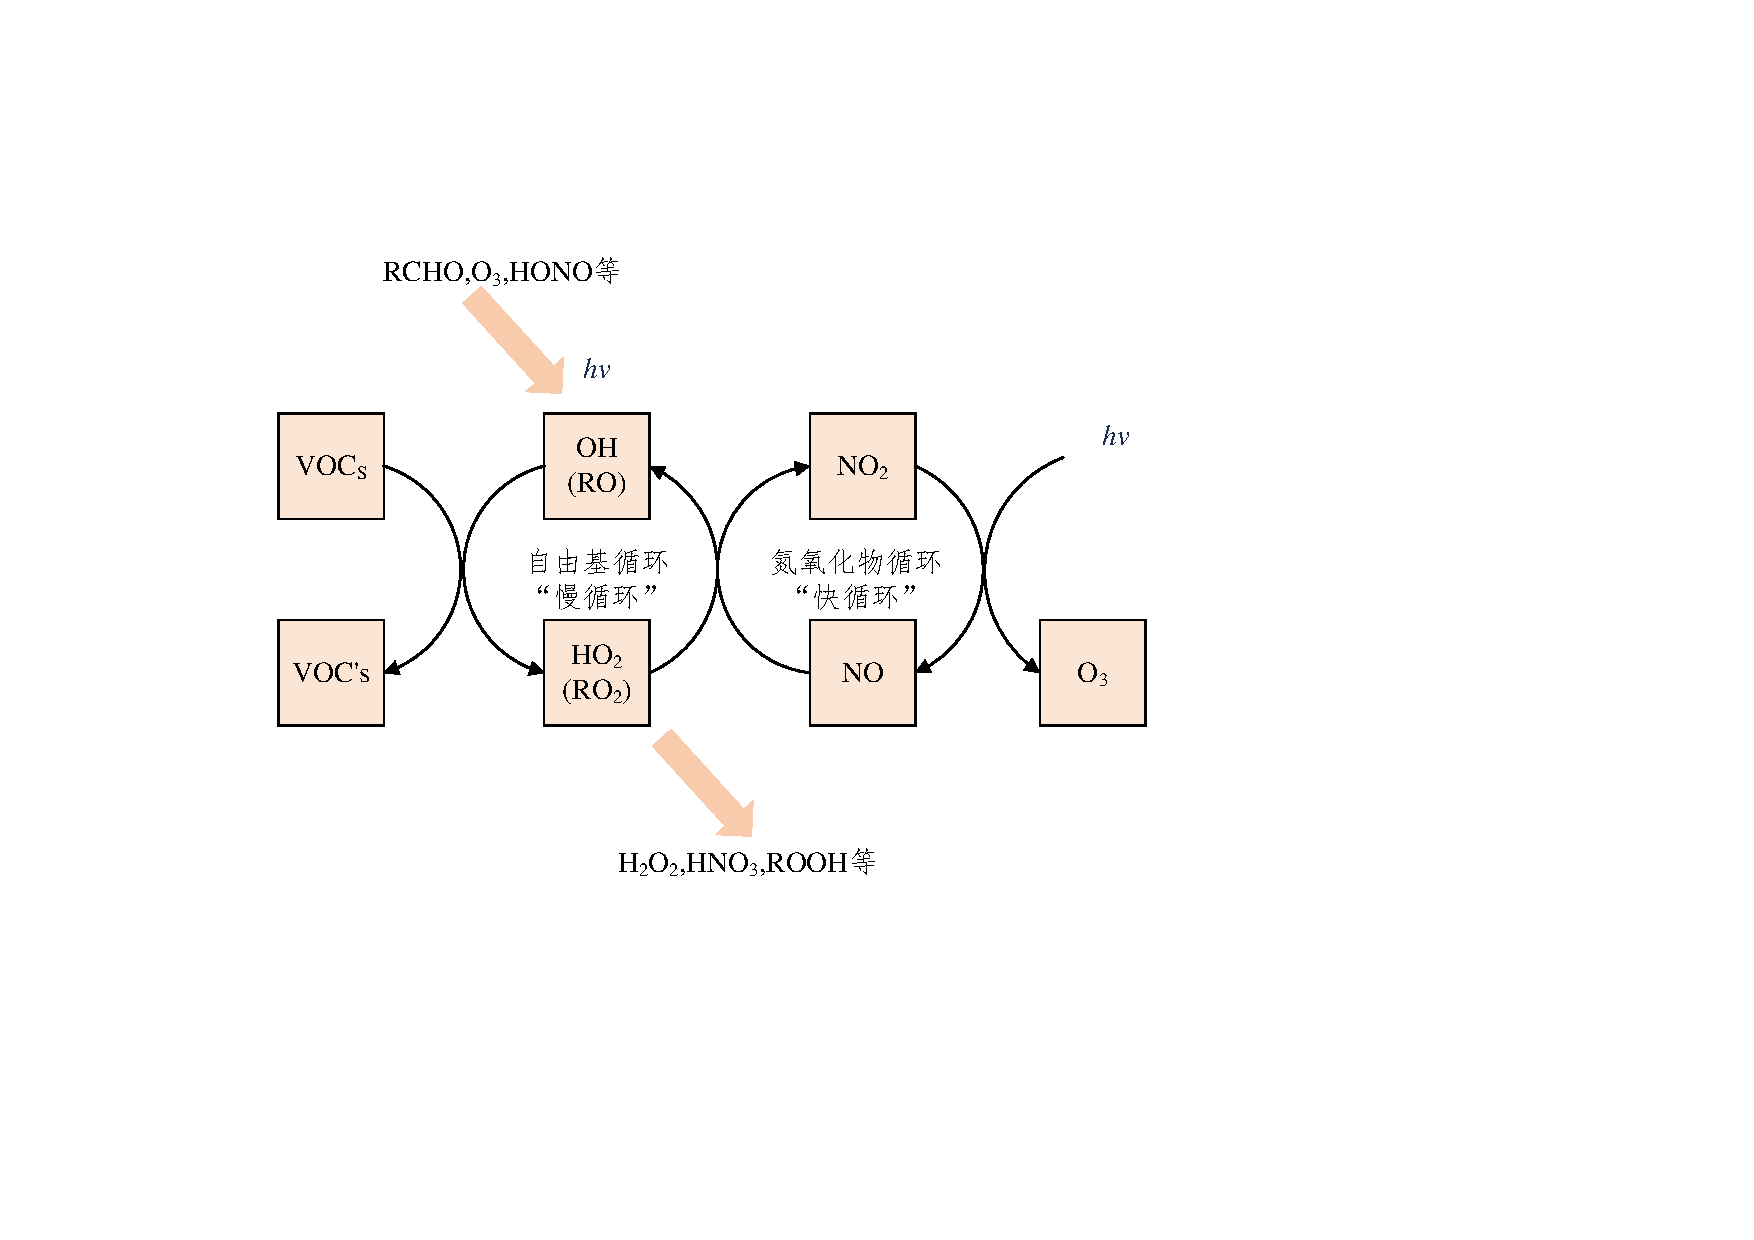
\includegraphics[width=.6\textwidth]{Gen_O3.pdf}
  }
  \caption{臭氧与氮氧化物之间相互转化的反应过程}\label{fig_O3}
\end{figure}


\subsection{模型求解和分析}


% Table generated by Excel2LaTeX from sheet 'Sheet1'
\begin{table}[htbp]
  \centering
  \caption{污染物浓度及AQI预测结果}
    \begin{tabular}{ccrrrrrrrr}
    \toprule
    \multirow{3}[2]{*}{预报日期} & \multirow{3}[2]{*}{地点} & \multicolumn{8}{c}{二次模型日值预测} \\
          &       & \multicolumn{1}{c}{SO2 } & \multicolumn{1}{c}{NO2 } & \multicolumn{1}{c}{PM10 } & \multicolumn{1}{c}{PM2.5 } & \multicolumn{1}{c}{O3最大八小时滑动平均} & \multicolumn{1}{c}{CO} & \multicolumn{1}{c}{\multirow{2}[1]{*}{AQI}} & \multicolumn{1}{c}{\multirow{2}[1]{*}{首要污染物}} \\
          &       & \multicolumn{1}{c}{(μg/m³)} & \multicolumn{1}{c}{(μg/m³)} & \multicolumn{1}{c}{(μg/m³)} & \multicolumn{1}{c}{(μg/m³)} & \multicolumn{1}{c}{ (μg/m³)} & \multicolumn{1}{c}{ (mg/m³)} &       &  \\
    \midrule
    2021/7/13 & 监测点A  &       &       &       &       &       &       &       &  \\
    2021/7/14 & 监测点A  &       &       &       &       &       &       &       &  \\
    2021/7/15 & 监测点A  &       &       &       &       &       &       &       &  \\
    2021/7/13 & 监测点B  &       &       &       &       &       &       &       &  \\
    2021/7/14 & 监测点B  &       &       &       &       &       &       &       &  \\
    2021/7/15 & 监测点B  &       &       &       &       &       &       &       &  \\
    2021/7/13 & 监测点C  &       &       &       &       &       &       &       &  \\
    2021/7/14 & 监测点C  &       &       &       &       &       &       &       &  \\
    2021/7/15 & 监测点C  &       &       &       &       &       &       &       &  \\
    \bottomrule
    \end{tabular}%
  \label{tab:addlabel}%
\end{table}%




%--------------------问题四的模型建立与求解----------------------
\section{问题四的模型建立与求解}
\subsection{问题四的描述分析}
问题四希望我们充分考虑区域协同性,因为相邻区域的污染物往往具有一定的相关性,区域协同预报可能会提升空气质量预报的准确度。在对站点A进行检测的同时,也需要考虑站点A周围的三个检测点A1、A2、A3的数据,建立一个包含这四个站点的协同预报模型,并希望尽量缩小AQI的预测值的最大相对误差,最后将该模型与问题3建立的模型进行性能比较,并讨论协同预报模型的现实有效性。这是一个是时间序列预测模型,传统的时间序列预测模型,如状态空间模型 (SSMS)[2]和自回归(AR)模型,被设计成独立地拟合每个时间序列,但需要从业者在手动选择趋势、季节性和其他组件方面的专业知识。为了解决上述挑战,深度神经网络[3-6]被提出作为一种替代解决方案,其中递归神经网络(RNN)[7-9]被用于以自回归的方式建模时间序列。然而,由于梯度消失和爆炸的问题,RNNs很难训练出了名的[10]。尽管出现了各种变体,包括LSTM[11]和Gru[12],但这些问题 仍未得到解决。Transformer[1,14]作为一种全新的架构被提出,利用注意机制来处理一系列数据。与基于RNN的方法不同,变压器允许模型访问历史的任何部分,这使得它可能更适合获取具有长期依赖性的循环模式。但标准的Transformer的空间复杂度随输入长度L的二次增长,导致了直接对细粒度长时间序列建模的内存瓶颈。本文参考了文献{\color{red}[Enhancing]}的想法,把Transformer架构应用于时间序列预测,
\subsection{数学模型的建立}

\subsection{模型求解和分析}

% Table generated by Excel2LaTeX from sheet 'Sheet1'
\begin{table}[htbp]
  \centering
  \caption{Add caption}
    \begin{tabular}{ccrrrrrrrr}
    \toprule
    \multirow{3}[2]{*}{预报日期} & \multirow{3}[2]{*}{地点} & \multicolumn{8}{c}{二次模型日值预测} \\
          &       & \multicolumn{1}{c}{SO2 } & \multicolumn{1}{c}{NO2 } & \multicolumn{1}{c}{PM10 } & \multicolumn{1}{c}{PM2.5 } & \multicolumn{1}{c}{O3最大八小时滑动平均} & \multicolumn{1}{c}{CO} & \multicolumn{1}{c}{\multirow{2}[1]{*}{AQI}} & \multicolumn{1}{c}{\multirow{2}[1]{*}{首要污染物}} \\
          &       & \multicolumn{1}{c}{(μg/m³)} & \multicolumn{1}{c}{(μg/m³)} & \multicolumn{1}{c}{(μg/m³)} & \multicolumn{1}{c}{(μg/m³)} & \multicolumn{1}{c}{ (μg/m³)} & \multicolumn{1}{c}{ (mg/m³)} &       &  \\
    \midrule
    2021/7/13 & 监测点A  &       &       &       &       &       &       &       &  \\
    2021/7/14 & 监测点A  &       &       &       &       &       &       &       &  \\
    2021/7/15 & 监测点A  &       &       &       &       &       &       &       &  \\
    2021/7/13 & 监测点A1 &       &       &       &       &       &       &       &  \\
    2021/7/14 & 监测点A1 &       &       &       &       &       &       &       &  \\
    2021/7/15 & 监测点A1 &       &       &       &       &       &       &       &  \\
    2021/7/13 & 监测点A2 &       &       &       &       &       &       &       &  \\
    2021/7/14 & 监测点A2 &       &       &       &       &       &       &       &  \\
    2021/7/15 & 监测点A2 &       &       &       &       &       &       &       &  \\
    2021/7/13 & 监测点A3 &       &       &       &       &       &       &       &  \\
    2021/7/14 & 监测点A3 &       &       &       &       &       &       &       &  \\
    2021/7/15 & 监测点A3 &       &       &       &       &       &       &       &  \\
    \bottomrule
    \end{tabular}%
  \label{tab:addlabel}%
\end{table}%

%--------------------模型评价----------------------
\section{模型评价}

\subsection{模型的优点}

\subsection{模型的缺点}

\subsection{模型的改进和展望}

%--------------------参考文献----------------------
%这里我使用了非bibTeX格式,B站教程:https://www.bilibili.com/video/BV1QL4y1Y7JR?spm_id_from=333.999.0.0
\addcontentsline{toc}{section}{参考文献} %将参考文献放进目录
% chenkangxin
\begin{thebibliography}{10}
% qiangzibro
% xiemin
\bibitem{ref1}郝吉明, 马广大, 王书肖. 大气污染控制工程 [M]. 北京: 高等教育出版社, 2010.
\bibitem{ref2}Rubin, Donald B. Inference and missing data. ETS Research Bulletin Series, 1975.
\bibitem{ref3}Mei, Gang, Nengxiong Xu, and Liangliang Xu. Improving GPU-accelerated adaptive IDW interpolation algorithm using fast kNN search. Springerplus 5.1 (2016): 1-22.
\bibitem{ref4}Shukla, Satya Narayan, and Benjamin M. Marlin. Interpolation-prediction networks for irregularly sampled time series. arXiv preprint arXiv:1909.07782 (2019).
\bibitem{ref5}Solanki, H. U., Dhyey Bhatpuria, and Prakash Chauhan. "Applications of generalized additive model (GAM) to satellite-derived variables and fishery data for prediction of fishery resources distributions in the Arabian Sea." Geocarto international 32.1 (2017): 30-43.
\bibitem{ref6}贺祥,林振山. 基于GAM模型分析影响因素交互作用对${PM_{2.5}}$浓度变化的影响[J]. 环境科学,2017,38(01):22-32.
\bibitem{ref7}Li, Shiyang, Xiaoyong Jin, Yao Xuan, Xiyou Zhou, Wenhu Chen, Yu-Xiang Wang, and Xifeng Yan. “Enhancing the Locality and Breaking the Memory Bottleneck of Transformer on Time Series Forecasting.” ArXiv:1907.00235 [Cs, Stat], January 3, 2020. http://arxiv.org/abs/1907.00235.
\bibitem{ref8}刘昕, 辛存林. 陕甘宁地区城市空气质量特征及影响因素分析. 环境科学研究, 2019, 32(12): 2065-2074.

\end{thebibliography}

%--------------------附录----------------------
\newpage

\appendix

\section{主程序源代码}

\begin{lstlisting}[language=Python]%设置不同语言即可。
kk=2;[mdd,ndd]=size(dd); %删除了会报错
# 问题1
print("Hello World!")
# 问题2
print("Open source is awesome!")
# 问题3
print("Open by NBU Professional Team" )
# 问题4

\end{lstlisting}


\end{document}